 \documentclass[DIV12,11pt,a4paper,titlepage,twoside,headings=small]{scrbook}
 %\usepackage[utf8]{inputenc}
\usepackage[english]{babel}
\usepackage[T1]{fontenc}


\def\TCop{\textsuperscript{\textcopyright}}
\def\TReg{\textsuperscript{\textregistered}}
\def\TTra{\textsuperscript{\texttrademark}}
\usepackage[latin1]{inputenc}
%\usepackage[utf8]{inputenc}
\usepackage{color}
\usepackage{colortbl}
%
\usepackage{fancyhdr}
\pagestyle{fancy}

\renewcommand{\chaptermark}[1]{%
 \markboth{\thechapter.\ #1}{}}

\renewcommand{\sectionmark}[1]{\markright{}}

\newcommand{\helv}{%
\fontfamily{phv}\fontsize{10}{11}\selectfont}

\fancypagestyle{plain}{%
%\fancyhf{} % clear all header and footer fields
\fancyfoot[C]{\helv \thepage} % except the center
%\renewcommand{\headrulewidth}{0pt}
\renewcommand{\footrulewidth}{0pt}}
\fancyfoot[C]{\helv \thepage} 


\fancypagestyle{plain2}{
	\fancyhf{}
	\fancyhead[C]{}
	\fancyfoot[C]{\thepage{}}
	\renewcommand{\headrulewidth}{1pt}
}
%\newenvironment{keeppage}{\let\thispagestyle{plain}}

 
\renewcommand{\chapterheadstartvskip}{\vspace *{-\baselineskip }}




\usepackage{setspace}

\usepackage{booktabs}
\usepackage{cite}
%\usepackage[numbers,sort&compress]{natbib}%enhanced citation
\usepackage[format=plain,footnotesize,labelfont=bf,justification=justified,singlelinecheck=false]{caption}
\usepackage{longtable}

\usepackage{tabularx}
\usepackage[section]{placeins}
\usepackage{geometry}
\usepackage{amsmath}
\usepackage{textcomp}
\usepackage{changepage}
\usepackage{lscape}

\renewcommand{\familydefault}{\sfdefault}
\usepackage{helvet}
     
\setstretch{1.4}
%\doublespacing

\parindent0pt
\usepackage{ifpdf}

%%% Should be LAST usepackage-call!
%%% For docu on that, see reference on package ``hyperref''
\ifpdf%   (definitions for using pdflatex instead of latex)

  %%% graphicx: support for graphics
  \usepackage[pdftex]{graphicx}

  \pdfcompresslevel=9

  %%% hyperref (hyperlinks in PDF): for more options or more detailed
  %%%          explanations, see the documentation of the hyperref-package
  \usepackage[%
    %%% general options
    pdftex=true,      %% sets up hyperref for use with the pdftex program
    %plainpages=false, %% set it to false, if pdflatex complains: ``destination with same identifier already exists''
    %
    %%% extension options
    backref,      %% adds a backlink text to the end of each item in the bibliography
    pagebackref=false, %% if true, creates backward references as a list of page numbers in the bibliography
    colorlinks=false,   %% turn on colored links (true is better for on-screen reading, false is better for printout versions)
    %
    %%% PDF-specific display options
    bookmarks=true,          %% if true, generate PDF bookmarks (requires two passes of pdflatex)
    bookmarksopen=false,     %% if true, show all PDF bookmarks expanded
    bookmarksnumbered=false, %% if true, add the section numbers to the bookmarks
    %pdfstartpage={1},        %% determines, on which page the PDF file is opened
    pdfpagemode=None         %% None, UseOutlines (=show bookmarks), UseThumbs (show thumbnails), FullScreen
  ]{hyperref}

\hyphenpenalty=10000
\exhyphenpenalty=10000
\sloppy

%%%%defines bibliography environment 
\def\thebibliography#1{\chapter{Bibliography}% 
    \markboth{Bibliography}{Bibliography} 
  \list{[\arabic{enumi}]}{\settowidth\labelwidth{[#1]}\leftmargin 
\labelwidth 
    \advance\leftmargin\labelsep 
    \usecounter{enumi}} 
    \def\newblock{\hskip .11em plus .33em minus .07em} 
    \sloppy\clubpenalty4000\widowpenalty4000 
    \sfcode`\.=1000\relax} 



  \DeclareGraphicsExtensions{.pdf}

\else %else   (definitions for using latex instead of pdflatex)

  \usepackage[dvips]{graphicx}
  

  \DeclareGraphicsExtensions{.eps}

%  \usepackage[%
%    dvips,           %% sets up hyperref for use with the dvips driver
%    colorlinks=false %% better for printout version; almost every hyperref-extension is eliminated by using dvips
%  ]{hyperref}

\fi

\usepackage{chngcntr}
\counterwithin{figure}{chapter}

\geometry{inner=3.0cm,outer=2.5cm}

\graphicspath{{Abbildungen/}}
\raggedbottom


\begin{document}


%\usepackage[T1]{fontenc}
%\newcommand{\changefont}[3]{
%\fontfamily{#1} \fontseries{#2} \fontshape{#3} \selectfont}
%\changefont{phv}{m}{n}

% title pages
%\chapter{Titelseite}
%\documentclass[a4paper, 12pt]{article}
%\usepackage[english]{babel}
%\usepackage{graphicx}
%\makeatletter
%\def\ScaleIfNeeded{%
%	\ifdim\Gin@nat@width>\linewidth
%		\linewidth
%	\else
%		\Gin@nat@width
%	\fi
%}
%\makeatother
%\def\TCop{\textsuperscript{\textcopyright}}
%\def\TReg{\textsuperscript{\textregistered}}
%\def\TTra{\textsuperscript{\texttrademark}}
%\usepackage[applemac]{inputenc}
%\usepackage{color}
%\pagestyle{headings}


%\newpage
%\usepackage[T1]{fontenc}
%\newcommand{\changefont}[3]{
%\fontfamily{#1} \fontseries{#2} \fontshape{#3} \selectfont}
%\changefont{phv}{m}{n}

%\begin{document}
\begin{titlepage}
\sffamily
\raggedleft

\begin{center}
\vspace*{1.5cm}

{\large
Inaugural - Dissertation \\
submitted to the \\ 
Combined Faculty for the Natural Sciences and for Mathematics \\ 
of the Ruperto-Carola University of Heidelberg, Germany \\ for the degree of\\
Doctor of Natural Sciences
}

\vspace{7cm}

presented by\\[2ex]
\textbf{\Large Tim Heinemann, M.S.} \\
Born in: Frankfurt (Oder)

\large Date of oral examination: 26$^{\text{th}}$ of March 2015 \\
\end{center}
\end{titlepage}

\clearpage{\pagestyle{empty}\cleardoublepage}

\newpage

%\newline
%\par
\begin{center}

\vspace*{1.5cm}

\fontsize{18pt}{20pt} \bfseries Robust Regulation of DNA Repair

\end{center}

\vfill
\begin{center}

\begin{tabular}{ l  l }
\renewcommand{\arraystretch}{1.5}
  %\multicolumn{2}{|c|}{Team sheet} \\
  Referees: &   \textbf{Prof. Dr. Thomas H�fer} \\ 

		  &	\textbf{Prof. Dr. Ursula Kummer} \\
		  
\end{tabular}
\end{center}


\thispagestyle{empty}
\newpage
\clearpage{\pagestyle{empty}\cleardoublepage}

%\textbf{Declaration}\\	
%\noindent The applicant, Tim Heinemann, declares that he is the sole author of the submitted dissertation and no other sources or materials from those specifically referred to have been used.\\ 
%In addition, the applicant declares that he has not applied for permission to enter
%examination procedure at another institution and this dissertation has not been presented to other faculties and not used in its current or in any other form in another examination.\\
%\\
%\\
%%\end{document}

%\begin{tabular}{p{10mm}>{\centering}p{50mm}p{10mm}
%>{\centering}p{50mm}p{10mm}}
%
%&\textit{Heidelberg, \today}&&\hrulefill& \\
%&\small Place, Date &&\small Tim Heinemann&
%\end{tabular}




% ************************* Acknowledgments *****************************

%\chapter*{Acknowledgements}
\addcontentsline{toc}{chapter}{Acknowledgements}
\thispagestyle{plain2}


An erster Stelle m\"ochte ich mich zutiefst bei meinem Betreuer Thomas H\"ofer f\"ur seine fortw\"ahrende Unterst\"utzung im Rahmen meiner Doktorarbeit  bedanken. Es lie\ss{}e sich nicht \"ubersch\"atzen, welch positiv inspirierenden Einfluss er auf diese Arbeit aber vor allem auch auf meine pers\"onliche wissenschaftliche Entwicklung genommen hat. \\

Ein gro\ss{}er Dank gilt Ursula Kummer und Frank Westermann f\"ur ihre kritische und zugleich motivierende Begleitung der Doktorarbeit als TAC-Mitglieder. Ursula Kummer gilt ein zus\"atzlicher Dank f\"ur ihre Rolle als Gutachterin der Arbeit und Vorsitzende des Pr\"ufungskomitees.\\

Ich bedanke mich sehr herzlich bei Prof. Ursula Klingm\"uller und Prof. Karsten Rippe f\"ur ihre Bereitschaft zur Teilnahme am Pr\"ufungskomitees.\\

Mein gr\"o\ss{}ter Dank gilt meiner Familie f\"{u}r ihren bedingungslosen R\"{u}ckhalt, ihr Vertrauen und ihr Liebe.\\

Ein herzliches Dankesch\"{o}n gilt Melanie, die nicht nur f\"{u}r meine gesunde Ern\"{a}rung, mein sportliches Wohlbefinden und meine regelm\"{a}\ss{}ige Teilnahme am Gruppenmeeting gesorgt hat, sondern auch eine gro\ss{}artige Freundin geworden ist. \\      

Ein weiterer gro\ss{}er Dank gilt Erika für ihre Freundschaft und für die vielen gemeinsamen Wanderungen um die Welt (und Heidelberg), die hoffentlich auch in Zukunft ihre Fortsetzung finden werden.\\

In ganz besonderem Ma\ss{}e m\"{o}chte ich mich bei Paul Verbruggen bedanken f\"ur seine Begeisterungsf\"{a}higkeit, seine Hartn\"{a}ckigkeit und seinen Humor, den er trotz des Amsterdamer Wetters nie verloren hat. Nicht oft hat man das Gl\"{u}ck mit einem Freund zusammenarbeiten zu d\"{u}rfen.\\

Einen gro\ss{}en Dank an Martin, der es trotz seiner Unerreichbarkeit irgendwie geschafft hat, immer f\"{u}r mich da zu sein.\\

Ich danke der gesamten Arbeitsgruppe H\"{o}fer f\"{u}r eine ausgesprochen angenehme Arbeitsatmosph\"{a}re.  
%\addcontentsline{toc}{part}{Acknowledgments}

\thispagestyle{plain}
%\clearpage{\pagestyle{empty}\cleardoublepage}

% *************************table of contents*****************************
%\setcounter{tocdepth}{3} %number gives depth of Table of Content 1 = only chapters, 2 = chapters + sections....
%\fancyhf{}
\thispagestyle{plain}
\pagenumbering{gobble}
\tableofcontents

%\tableofcontents
%\thispagestyle{plain}
%\newpage



%\clearpage{\pagestyle{empty}\cleardoublepage}

% main part
%\mainmatter

%\clearpage{\pagestyle{empty}\cleardoublepage}
%\thispagestyle{empty}
%\cleardoublepage

%\pagestyle{fancy} \lhead[\normalsize\thepage\hfill\footnotesize
%\thechapter \hspace{2pt} \leftmark\ ]{} \chead{}
%\rhead[]{\footnotesize\thesection \hspace{2pt}
%\rightmark\hfill\normalsize\thepage} \lfoot{} \cfoot{} \rfoot{}

%\thispagestyle{empty}





% ************************* Abtract1 *****************************



%\renewcommand{\sectionmark}[1]{\markright{}}

\chapter*{Zusammenfassung}
\thispagestyle{plain2}
\addcontentsline{toc}{chapter}{Zusammenfassung}
\pagenumbering{roman}


DNA-Reparaturmechanismen sind unabdingbar, um die Zelle gegen innere und \"{a}u\ss{}ere Einfl\"{u}ssen zu sch\"{u}tzen. Dies \"{a}u\ss{}ert sich in einer erh\"{o}hten Anf\"{a}lligkeit f\"{u}r Zellalterung und Krebsentwicklung infolge eines beeintr\"{a}chtigten Reparaturapparats. Der Reparaturprozess wird von enzymatisch aktiven, makromolekularen Komplexen ausgef\"{u}hrt, die sich an gesch\"{a}digten Chromatinfasern assemblieren. Fluoreszenzmikroskopische Untersuchung\-en einzelner Reparaturfaktordynamiken haben gezeigt, dass die Komplexbildung durch einen schnellen Proteinaustausch charakterisiert ist, wohingegen die Gesamtreparaturzeit wesentlich l\"{a}nger ausf\"{a}llt. Inwiefern die schnellen Austauschkinetiken zur Regulation von \"{u}bergeordneten Systemeigenschaften, wie z.B. der Reparaturrate und deren Robustheit, beitragen, ist bisher nur unzureichend verstanden.\\
In dieser Arbeit quantifizieren wir die Beziehung der Proteindynamiken und ihren Einfluss auf den Reparaturprozess durch die zeitaufgel\"{o}ste Messung der Nukleotidexzisionsreparatur (NER) in S\"{a}ugerzellen. Wir finden heraus, dass es sich bei der DNA Reparatur, ungeachtet der Komplexit\"{a}t der grundlegenden molekularen Prozesse, um eine langsame Reaktion erster Ordnung mit einer Halb\-wertzeit von 1.2 Stunden handelt. 
Um einen funktionellen Einblick zu bekommen, entwickeln wir ein identifizierbares ma\-the\-matisches Modell des NER Reaktionsweges. Eine wichtige Vorhersage des Modells ist, dass die Reparatursynthese nicht von einer ratenlimitierenden Komponente allein kontrolliert wird. Vielmehr zeigen alle Reparaturfaktoren einheitlich niedrige Kontrollkoeffizienten, und tragen daher gemeinsam zur Kontrolle der Reparaturrate bei. Durch Ausnutzen der nat\"{u}rlichen Proteinexpressionsvariabilit\"{a}t zwischen Einzelzellen k\"{o}nnen wir die Modell\-vorhersage einer verteilten Kontrolle der Reparaturrate f\"{u}r die NER-Faktoren XPC, TFIIH, XPA, XPF und RPA experimentell qualitativ best\"{a}tigen. Quantitativ ist die gemessene durchschnittliche Antwort der Reparaturrate jedoch signifikant h\"{o}her als der vorausgesagte mittlere Responsekoeffizient. Auf der Suche nach weiteren Quellen, die zur Kontrolle der Reparaturrate beitragen, beobachten wir eine starke positive Korrelation der nu\-klearen NER-Faktor-Konzentrationen, was auf einen komplement\"{a}ren Kontrollmechanismus zur Regulierung dieser Proteinkonzentrationen hinweist. Beachtenswert ist, dass sich die Diskrepanz zwischen gemessener und vorausgesagter Reparaturantwort aufl\"{o}\ss{}t, wenn die Kontrollanalyse um die gemessenen Kreuzkorrelationen erweitert wird.\\              
Die hier gewonnenen Erkenntnisse zeigen zwei einander erg\"{a}nzende Regulationsmechanismen der DNA-Reparatur auf. Im ersten Mechanismus generiert die Stochastizit\"{a}t der Proteinaustauschdynamiken eine lange Zeitskala, die Heterogenit\"{a}ten der nu\-klearen Vorkommen einzelner NER-Faktoren kompensiert. Im zweiten Mechanismus, dessen molekulare Details unbekannt sind, wird die NER-Faktorexpression selbst kontrolliert. Da chromatinassoziierte Prozesse wie z.B. Chromatinremodellierung, Transkription und Translation ein \"{a}hnliches dynamische Design wie die DNA Reparatur besitzen, k\"{o}nn\-ten sich diese beiden grundlegenden Mechanismen als allgemeine Kontrollmodi f\"{u}r Chromatindynamiken erweisen.  


  





%\addcontentsline{toc}{part}{Zusammenfassung}

%\thispagestyle{empty}
%\clearpage{\pagestyle{empty}\cleardoublepage}


% ************************* Abtract2 *****************************
\chapter*{Summary}
\thispagestyle{plain2}
\addcontentsline{toc}{chapter}{Summary}





DNA repair is indispensable for the intracellular protection against environmental and endogenous damaging agents. This is reflected in an increased susceptibility to cellular ageing and cancer development as a consequence to impaired repair. The repair process is carried out by enzymatic macromolecular complexes assembling at damaged sites on the chromatin fibre. Fluorescence imaging of the individual repair factor dynamics show a rapid protein exchange at the repair sites, while the overall repair time is significantly longer. How these fast molecular interactions regulate the emergence of higher-level system-properties, such as the repair rate and its robustness, is poorly understood.\\ 
In this thesis we quantify the relation between the protein dynamics and the resulting repair by measuring the time course of nucleotide-excision DNA repair (NER) in mammalian cells. We find that, despite the pathway's molecular complexity, DNA repair follows a slow first-order reaction with a half-time of 1.2 hours. To gain functional insight, we develop an identifiable mathematical model of the NER pathway. According to a model prediction repair synthesis is not controlled by one rate-limiting component alone. Instead, all NER factors collectively control the repair-rate, as indicated by uniformly small response coefficients. Harnessing the natural cell-to-cell variability of protein expression, we show qualitative experimental support for the shared control of the core NER factors XPC, TFIIH, XPA, XPF and RPA. However, quantitatively the measured average repair-rate response is significantly larger than the predicted mean response coefficient. In search of additional sources contributing to the repair-rate control, we observe that the nuclear NER factor expression is strongly correlated suggesting a complementary control mechanism regulating these protein expression values. Notably, the discrepancy between measured and predicted repair-rate response is resolved by including the identified cross-correlation in the control analysis. \\ 
These findings portray two complementary modes of robust regulation in DNA repair. One, where the long time-scale of the repair-complex assembly, generated by the stochastic nature of the protein exchange dynamics, compensates for heterogeneities in the nuclear abundance of single repair proteins. And a second, mechanistically unknown mode controlling the nuclear NER factor expression itself. Given that chromatin remodelling, transcription and translation have similar dynamic features as DNA repair, both mechanisms may function as widespread modes of robust regulation of chromatin-associated processes.



%provide a rationale for the emergence of slow time scales in chromatin-associated processes from fast molecular steps and suggest that collective rate control might be a widespread mode of robust regulation in DNA repair and transcription.
      
 


%\end{document}
%\addcontentsline{toc}{part}{Summary}

%\thispagestyle{empty}
%\clearpage{\pagestyle{empty}\cleardoublepage}



% ************************* PART I *****************************

\chapter{Introduction}
\pagenumbering{arabic}
\pagestyle{plain}

\section{DNA damage and its consequences}

The impeccable preservation of DNA is surely one of the most essential requirements for cellular viability. On a single day DNA accumulates on average $\sim\text{10}^\text{5}$ damages per cell, which can be grouped into three different categories \cite{Hoeijmakers2009}. First, DNA constantly undergoes spontaneous unspecific reactions (mostly hydrolysis) that cause deamination and create abasic sites in an aqueous solution \cite{Lindahl1993,Lhomme1999}. Second, the most common type of DNA damage originates from the cellular metabolism, which produces various types of reactive oxygen and nitrogen species,lipid peroxidation products, endogenous alkylating agents, estrogen and cholesterol metabolites, and reactive carbonyl species. The subsequent molecular distortions range from several kinds of single-strand breaks to various oxidative base and sugar products \cite{DeBont2004,Sander2005}. And third, DNA damages that are caused by external physical or chemical agents like sunlight, which induces approximately 30,000 pyrimidine dimers per hour in each exposed keratinocyte \cite{Luijsterburg2010}.\\        
The consequences for the cellular viability that arise from the diversity of DNA lesions are essentially twofold. Either, the inflicted chromosomal aberrations are not recognized or bypassed by the DNA repair machinery and thus persist in the genetic Code \cite{Hoeijmakers2009}. These mutations can activate oncogenes or inactivate tumour suppressor genes, which is equivalent to an increase in the cell's cancer risk level \cite{Bartek2007}. Or, alternatively, the damage is so strong that essential cellular processes such as transcription or replication are impaired. This is usually the case for interstrand cross-links or double-strand breaks induced by ionizing irradiation. The occurrence of such lesions leads to accelerated cell death, which particularly in proliferative tissues promotes symptoms of premature ageing \cite{Marteijn2014}. Depending on the location and number of lesions, the cell type, stage in the cell cycle and differentiation both outcomes can happen concurrently. In fact, both cell fates are directly linked considering that damage-induced cell-death protects the body from cancer \cite{Hoeijmakers2009}.            

\paragraph{DNA damage response}    
DNA is the only known biological macromolecule, which cannot be replaced if parts of it are destroyed. This has the inevitable consequence that any mutation that escapes cell-death will persist over the lifetime of the cell \cite{Hoeijmakers2009,Marteijn2014}. For this reason, cells evolved an elaborate genomic maintenance apparatus, the DNA damage response (DDR), that keeps DNA damage under control \cite{Ciccia2010}. The DDR system not only includes various DNA-damage sensors and the enzyme machinery catalysing the individual repair reactions. It also  involves a prophylaxis mechanism through tanning; it regulates a range of downstream mediators and signalling molecules that control cell cycle state and cell fate and most importantly it comprises a number of complementary repair systems, each of which responsible for a specific type of damage \cite{Ciccia2010,Marteijn2014}. Subtle chemical alterations like oxidative lesions and alkylation products are removed by base-excision repair (BER) \cite{Lindahl2000,Caldecott2008}. More complex lesions like interstrand crosslinks (ICLs) or helix distorting lesions are repaired by ICL repair or nucleotide excision repair, respectively \cite{Moldovan2009,Hoeijmakers2009}. Entire cuts of the DNA are processed either by nonhomologous end joining (NHEJ) or homologous repair (HR) \cite{Caldecott2008,West2003}. 

\paragraph{Spatiotemporal regulation of DNA repair} For all repair mechanisms their spatiotemporal regulation follows the general organization of chromatin-associated processes: a) detection of the target site (\textit{e.g.} a DNA lesion) b) assembly of the repair components to a multi-protein complex at the DNA and c) catalysis of an enzymatic reaction with the DNA as a substrate \cite{Hoeijmakers:2001:Nature:11357144,Gillet:2006:Chem-Rev:16464005,Dinant:2009:J-Cell-Biol:19332890,Luijsterburg2010}. Of much interest is thereby the role of the assembly phase, which was, until recently, understood as a sequential, cooperative recruitment of components \cite{Volker2001}. A competing perception considers the complex formation as a combined process of randomly diffusing and rapidly exchanging components \cite{Luijsterburg2010}. This is supported by experimental evidence for DNA repair but also transcription initiation showing that dissociation and rebinding for the constituents of the respective complexes occur on the seconds to minutes time scale \cite{Vermeulen2011,Stasevich2011}. Similar findings are reported for the clustering of RNA polymerases and for replication, with the exception of stably bound Mcm proteins that determine licensed replication origins \cite{Kuipers2011,Sonneville2012}. However, it remains poorly understood how the dynamic interplay of these multi-protein machineries effects the formation of essential system properties like fidelity, timing and robustness. 




\section{NER as a model system for chromatin-associated processes}
\label{sec:NERexperiments}
To gain more insight into the assembly and functioning of protein complexes we have studied the mammalian nucleotide excision repair (NER) pathway. NER is involved in the elimination of a wide range of structurally unrelated DNA lesions, including cyclobutane-pyrimidine dimers (CPDs) and 6-4 pyrimidine-pyrimidone photoproducts (6-4PPs), both induced by ultraviolet (UV) light; various bulky chemical adducts (man-made and natural); intrastrand crosslinks caused by drugs such as cisplatin; and ROS-generated cyclopurines \cite{Marteijn2014}. Consequently, the NER machinery is in itself a composition of intertwined repair mechanisms, which give rise to an exceptional clinical heterogeneity associated with the impairment of NER components.


\paragraph{Molecular mechanism of NER}
The process of damage detection by NER is distinguished into transcription-coupled NER (TC-NER) \cite{Sugasawa:2005:Cell:15882621,Gillet:2006:Chem-Rev:16464005}, where bulky DNA adducts block the transcription machinery and global genome NER (GG-NER) where the same adducts are eliminated throughout the whole genome \cite{Fousteri2008}. In this work we will focus on GG-NER whose core repair factors are all identified and intensively studied. For GG-NER the initial lesion detection is performed by XPC \cite{Sugasawa:1998:Mol-Cell:9734359,Volker2001}. The binding of XPC promotes the association of the TFIIH (transcription initiation factor IIH) complex \cite{Yokoi:2000:J-Biol-Chem:10734143,Riedl2003,Volker2001}. TFIIH consists of 10 components out of which the subunits XPB and XPD have helicase activity with opposite polarity \cite{Tapias2004,Compe2012}. Upon DNA unwinding XPA can bind to altered nucleotides on the damaged single strand whereas the replication protein A (RPA) protects the undamaged strand. Alongside the endonucleases XPG and ERCC1/XPF excise approximately 30 nucleotides around the lesion \cite{Evans1997,deLaat:1998:Genes-Dev:9716411,Wakasugi:1997:J-Biol-Chem:9188507,Park:2006:FEBS-J:16623697,Camenisch:2006:Nat-Struct-Mol-Biol:16491090}. Subsequently, the proliferating cell nuclear antigen (PCNA) is loading the polymerase $\delta$, which refills single-strand DNA gap \cite{Hoeijmakers:2001:Nature:11357144,Essers2005,Moser:2007:Mol-Cell:17643379}. After ligation by LigIII-XRCCI the DNA strand is then rechromatinised by CAF1, which completes the repair process \cite{Green:2003:EMBO-J:14517254,Polo2006} (see Figure \textbf{tbm} for comparison). 

\begin{figure}[htbp]
	\begin{center}
		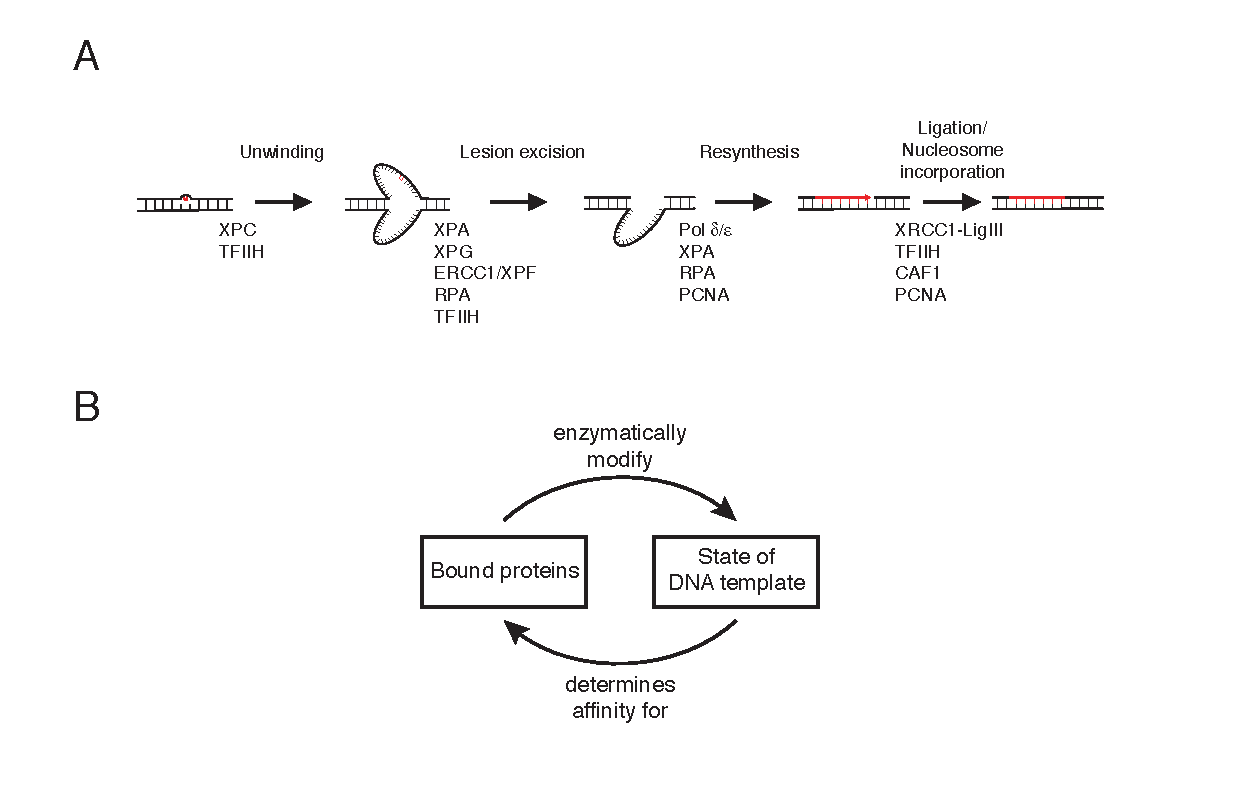
\includegraphics[width=1\textwidth]{Abbildungen/figure1_1.pdf}
		\caption{\textbf{NER as a paradigm for chromatin-associated processes.} A) Graphical scheme of the NER pathway. Shown is the sequence of repair intermediates together with the repair factors that, if fully assembled, catalyse the next reaction. B) 'Recruiting-reaction' cycle illustrating the principle of the sequential organization of chromatin-associated processes. Therein, recruited process components catalytically modify the DNA template and thereby redefine the binding affinity for the next complex.}
		\label{fig:introScheme}
	\end{center}
\end{figure} 

\paragraph{Data-driven kinetic modelling of NER}
Defects in GG-NER are associated with the prototypical nucleotide-excision-repair disorder xeroderma pigmentosum (XP), which is associated with pigmentation abnormalities and an increased risk of skin cancer and internal tumours \cite{Hoeijmakers2009}. XP is caused by gene-defects in one of the seven XP-genes, XPA through XPG. Despite the severe symptoms related to one of these defects all patients are viable, which allowed for the isolation of patient cell lines where the endogenous NER factor is knocked-out. More importantly, these cell lines could be transfected with a GFP-tagged construct of the missing protein enabling the fluorescence real-time measurement of the NER factor kinetics \cite{Hoogstraten2002,Hoogstraten2008,Zotter2006,Rademakers2003}. Taken together, the clearly defined UV-mediated inducibility of NER combined with the availability of the fluorescently-tagged core repair factors makes NER a paradigm for the research on chromatin-associated processes.\\
On the basis of accumulation and dissociation time courses for each NER factor Luijsterburg \textit{et.\ al.}\cite{Luijsterburg2010} developed a quantitative model of the NER process. This model suggests for the formation of enzymatically active protein complexes a cyclic principle (cf.\ Figure \textbf{tbm}B): Repair factors bind reversibly and assemble stochastically at the DNA template; once the complex is fully assembled it modifies the DNA substrate and thereby changes the binding affinity for the next enzymatic complex. Traversing multiple of these 'recruiting-reaction' cycles will translate the recurring stochastic protein exchange at the chromatin site into an ordered sequence of regulatory events \cite{Dinant:2009:J-Cell-Biol:19332890}.\\
This model unravels a number of interesting relations between assembly dynamics and process functionality, \textit{e.g.} that rapidly reversible protein binding allows for high specificity of the pathway through kinetic proofreading \cite{Luijsterburg2010}. In agreement to this notion, such combinations of live cell experiments and mathematical modelling have led to equally intriguing results for transcription. As indicated by Gorski \textit{et.\ al.} \cite{Gorski:2008:Mol-Cell:18498750} already a moderate increase in the dwell-time of RNA Pol I subunits caused the enhancement of the assembly efficiency and the initiation rate of RNA Pol I. Another study describes a mechanism termed 'assisted loading', where a weak transcription factor-DNA interaction facilitates the binding of a second transcription factor and thereby obviates the need for simultaneous and cooperative binding \cite{Voss2011}. \\         
A prevailing problem affecting the value of quantitative model predictions is concerned with the non-identifiability of the model parameters by the \textit{in vivo} data (on-rate and off-rate constants as well as enzymatic rate constants). As a consequence the parameter uncertainties are propagated to the model predictions, which limits their significance \cite{Raue2013}. To overcome these limitations further developments in the model-driven analysis of chromatin-associated processes will depend on the integration of model calibration, uncertainty analysis and experimental design.     
  

\section{Research objectives}

In the course of this study, we want to expand the theoretical analysis of the NER process and thereby increase our understanding of the interrelation between protein-complex assembly dynamics and the functionality of chromatin-associated machineries. This analysis will be guided by the following questions:

\begin{itemize}
	\item What is the quantitative relation between the 'recruitment-reaction' design principle of functional repair complexes and the overall repair kinetic of the DNA lesions?
	
	\item Which pathway components contribute to the control of the apparent repair rate? 
	
	\item Which molecular mechanisms are responsible for the robust regulation of DNA repair? 
\end{itemize} 

To start with, we extended the comprehensive information about protein dynamics measured previously with a time-resolved readout of DNA repair synthesis in individual living cells. The measured time course follows a slow first-order kinetic, which turned out to be compatible with the current understanding of rapidly reversible protein assembly. With the combined data set we were able to identify a realistic model of NER and thus to make quantitative predictions about the repair process. One particularly captivating model outcome disagrees with the existence of a rate-limiting repair factor but instead emphasises a shared and moderate control of the repair rate. Exploiting the natural variability in repair factor expression we found experimental support for this prediction. Intriguingly, the protein expression itself is correlated independent of the repair process and the cell cycle stage. This suggests that the robustness of DNA repair is regulated by a combination of collective NER factor rate control and a so far unknown pre-transcriptional mechanism.   









%\thispagestyle{empty}
%\clearpage{\pagestyle{empty}\cleardoublepage}

% ************************* PART II *****************************


\chapter{Fluorescence time-lapse imaging of the NER process}
\label{chap:quantData}
\pagestyle{plain}


Mon\'{e} and colleagues (2001) advanced the research on nucleotide excision repair (NER) essentially by developing a technique to UV-irradiate a cell's nucleus within a locally confined area \cite{Mone2001}. Until then, the \textit{in-vivo} analysis of NER was limited to measurements of enzyme mobility and exchange dynamics at steady state performed with photobleaching experiments after irradiation of the whole nucleus \cite{Houtsmuller2001,Mone2004,Vermeulen2011}. In contrast, the enclosed amount of single-stranded DNA damages causes the local activation of a multi-protein repair machinery, which in turn allows us to study the \textit{de-novo} assembly and dissociation kinetics of individual repair factors. Exploiting this standard experimental set-up, Luijsterburg \text{et.\ al.} collected a comprehensive time-series dataset comprising the accumulation and dissociation of seven individual repair enzymes.\\ 
In the following chapter we will introduce this data together with the experimental methods, which represent the basis for our quantitative analysis of the NER process. We were able to augment the measurements with a direct readout for newly-synthesized DNA following the incorporation of the fluorescently modified nucleotide analogue EdU. It turns out that the DNA repair process is essentially a slow first-order reaction with a half-life of 1.2 hours.   \\


The experiments reported in this chapter were planed and conducted by Martijn Luijsterburg (accumulation and FLIP experiments; Leiden University) and Paul Verbruggen (EdU incorporation; University of Amsterdam).
	
	


\section{Locally UV-inflicted DNA damage}
\label{sec:local_irradiation}
 

To observe the dynamic behaviour of NER factors upon local infliction of DNA damage, we applied the experimental set-up developed by Mon\'e \textit{et al.} (2001)\cite{Mone2001}, in which NER-competent cells are covered with a polycarbonate UV filter containing pores with a given diameter (cf.\ Figure \ref{fig:accuMethod}A). For our purposes, cells were grown on uncoated 24 mm coverslips before being overlaid with a mask with pores of 5 \textmu m diameter \cite{Verbruggen2014}. Figure \ref{fig:accuMethod}B illustrates the realistic deviation of pore diameters due to manufacturing inaccuracies. The expected size deviation has a very small coefficient of variation (CV) of 0.14 indicating a negligible effect on the filter's transmissivity. Filter-covered cells were immediately irradiated with a dose of 100 $\text{J/m}^\text{2}$ of UV-C with a fluency of 3.85 $\text{W/m}^\text{2}$. Due to the specific pore density (4 x $\text{10}^\text{5}$ pores/$\text{cm}^\text{2}$), we could observe nuclei containing only either one damage spot or no spot at all. Two spots per cell were only observed very rarely (cf.\ Figure \ref{fig:accuMethod}C, white arrows indicate the damage spot). With this technique we were able to measure DNA repair in damaged nuclei as well as undamaged control nuclei in the same experiment.

\begin{figure}[t!]
	\begin{center}
		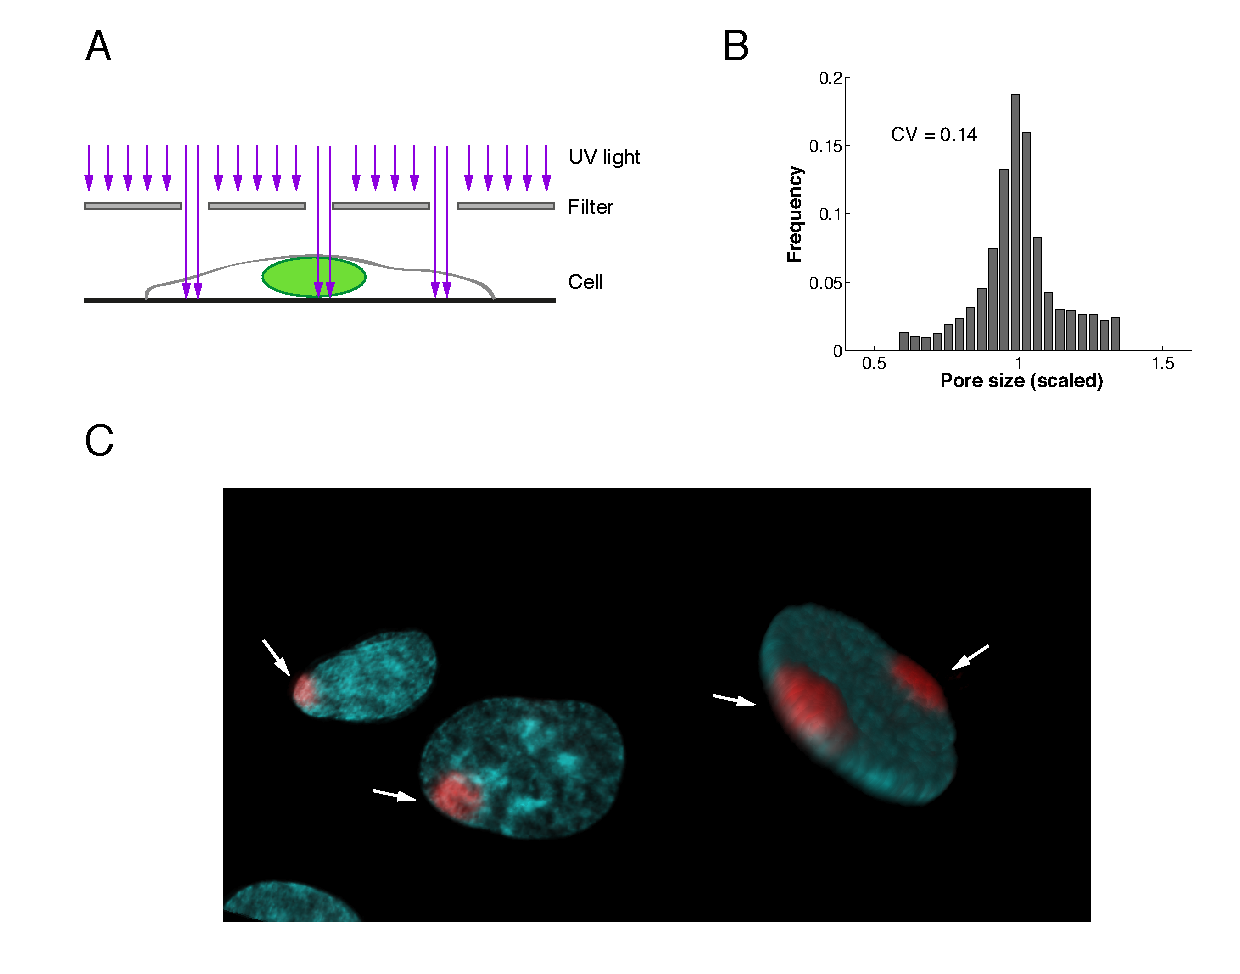
\includegraphics[width=1\textwidth]{Abbildungen/figure2_1.pdf}
		\caption{\textbf{Local irradiation leads to spatially confined DNA damage.} A) Schematic illustration of the experimental set-up. UV-light (purple arrows) is transmitted through a UV filter containing pores with 5 \textmu m diameter. Local irradiation of the chromatin occurs if a pore is located above a cell nucleus. (reprinted Figure from \cite{Terstiege2010}) B) Distribution of the pore sizes within the UV irradiation mask (n=5008) - \textbf{ask paul how he did it} C) Partially UV-irradiated nuclei of cultivated mammalian cells were made visible with a blue-fluorescent DNA stain. Red fluorescence depicts incorporation of labelled nucleotides due to NER.}
		\label{fig:accuMethod}
	\end{center}
\end{figure}

\section{Repair factor accumulation and dissociation occur on different time scales}
\label{subsec:AccuFlipExp}
The ability to locally inflict DNA damage with a discrete dose of UV-C allows for the study of accumulation and exchange behaviour of fluorescently-tagged repair proteins under different experimental conditions. In the following, we describe the comprehensive dataset acquired by Luijsterburg \textit{et al.} (2010)\cite{Luijsterburg2010}, which represents the basis for our quantitative analysis of the NER process. In total, the kinetics of seven repair factors were measured: i) XPC, the lesion recognition factor, ii) TFIIH, the helicase responsible for DNA unwinding, iii) XPA and RPA, which bind and thereby protect single stranded DNA against cleavage, iv) the exonucleases XPF/ERCC1 and XPG performing the incision of the damaged DNA strand and, v) PCNA, which loads the DNA polymerase and hence indirectly provides insight into the DNA repair-synthesis kinetics. \\
Each repair factor were exogenously tagged with a green fluorescent protein (GFP) (or its 'enhanced' derivative EGFP) and expressed at physiological levels within the cell nucleus. Before the cells have been UV-irradiated at time t = 0, the repair proteins were homogeneously distributed at steady state. Immediately afterwards, the repair factors accumulated at the damaged chromatin sites, which led to a higher visible fluorescence intensity (cf.\ Figure \ref{fig:accuImage}A). For quantification of the fluorescence intensity, image analysis was done by using ImageJ software (NIH Bethesda, MD). Accumulated repair-factor concentrations were determined by multiplying the nuclear reference concentrations (cf.\ Table \ref{tab:nuclearconcentrations}) with the fraction of bound proteins at damaged DNA:
% * <l.adlung@dkfz.de> 2014-12-06T23:21:59.631Z:
%
%  expressed at physiological levels under the endogenous promoter?
%
\begin{equation}
Bound \, fraction = (I_\text{LD} - I_\text{outspot})A_\text{LD}/ (I_\text{nucleus} - I_\text{background})A_\text{nucleus}
\label{Eqn:BoundFraction}
\end{equation}     
where $I_\text{LD}$, $I_\text{outspot}$, $I_\text{nucleus}$ and $I_\text{background}$ represent the average fluorescence intensities within the locally damaged spot, an equally sized area in the non-damaged nucleus, the whole nucleus and the background, respectively (cf.\ Figure \ref{fig:accuImage}B). $A_\text{LD}$ and $A_\text{nucleus}$ give the size of the damaged area and the size of the nucleus. Finally, the concentrations of accumulated protein are calculated assuming a damaged nuclear volume of 0.3 pL \cite{Luijsterburg2010}.\\    

 \begin{table}[h!]
 \centering
\begin{tabular}{ccc}
\hline
\textbf{Protein} & \quad \textbf{Concentration} \quad& \quad \textbf{Bound fraction}\\ \hline
XPC\hspace{1cm}&0.140 \textmu M&13\%\\ 
TFIIH&0.360 \textmu M&10\%\\  
XPG&0.440 \textmu M&9\%\\  
XPA&1.110 \textmu M&7\%\\  
\quad XPF/ERCC1 \quad&0.170 \textmu M&7\%\\  
RPA&1.110 \textmu M&15\%\\  
PCNA&1.110 \textmu M&20\%\\  \hline
\end{tabular}
 \caption{\textbf{Nuclear concentrations of NER factors (in \textmu M)} All nuclear quantities are based on published data or on previous estimates \cite{Araujo2001,Houtsmuller1999,Mone2004}. The nuclear concentrations were taken from Luijsterburg \textit{et.\ al.} \cite{Luijsterburg2010} were a nuclear volume of 0.3 pL was assumed. The bound fractions were determined by Eqn.\ \ref{Eqn:BoundFraction}. }\label{tab:nuclearconcentrations}
  \end{table}
% * <l.adlung@dkfz.de> 2014-12-06T23:29:58.578Z:
%
%  Precisely mention irradiation and cell type
%
  
During the timespan of DNA repair, NER factor concentrations rise at the sites of local damage and then gradually decrease from their plateau levels at different rates (cf.\ Figure \ref{fig:accuImage}C). For example, the half-time $t_\text{1/2}$ for XPC- and XPG-EGFP is $\sim$1 h whereas XPA-EGFP has a longer half-time of $\sim$2.5 h \cite{Luijsterburg2010}. In contrast, PCNA and RPA stay present in the damage spot even after lesion removal. These results show that NER factors engage for hours in the repair process with temporal changes in the molecular composition.\\
\begin{figure}[t!]
	\begin{center}
		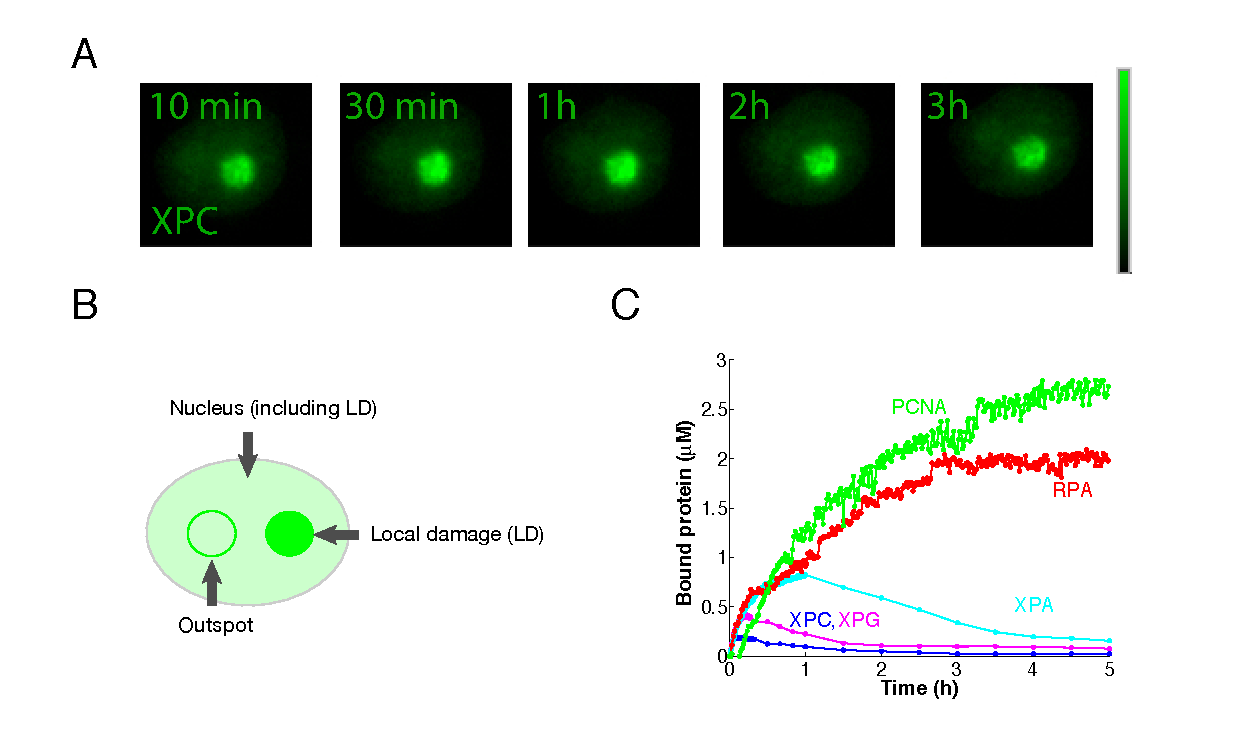
\includegraphics[width=1\textwidth]{Abbildungen/figure2_2.pdf}
		\caption{\textbf{Fluorescently labelled NER factors accumulate at locally irradiated nucleus.} A) XPC-eGFP  stably expressed in XP-C cells  after local irradiation with UV-C (100 J$\text{m}^{-\text{2}}$ through 5-\textmu m-diameter pores). XPC-eGFP accumulates at sites of local DNA damage.  B) Scheme of a locally UV-irradiated nucleus. Depicted are all regions relevant for signal quantification. C) Time courses of XPC-eGFP (n = 12), XPG-eGFP (n = 5), eGFP-XPA (n = 7), eGFP-PCNA (n = 5) and RPA-eGFP (n = 5) expression showing their accumulation at the local damage (LD) spot. For consistency only cell nuclei with one single damage spot were used.}
		\label{fig:accuImage}
	\end{center}
\end{figure}
To characterize the interaction between repair proteins and DNA intermediates, dwell times were determined by fluorescence loss in photobleaching (FLIP) experiments \cite{Luijsterburg2010}. Thereby, a large part of the nucleus, away from the local damage spot, is continuously bleached at 100\,\% laser power (cf.\ Figure \ref{fig:accuFlip}A, white rectangle). At the same time, fluorescent proteins are probed at low laser power (to prevent photobleaching) elsewhere within the nucleus. Repair proteins dissociating from the local damage spot have a high probability of being bleached before rebinding due to their large diffusivity. Accordingly, binding of the repair proteins seems to be rate limiting for the dwell time, not diffusing \cite{Luijsterburg2010}.\\
However, compared to the long timespan (in the order of hours) where repair protein levels are still elevated at the site of local damage, all NER factors dissociate very quickly from damaged DNA with half-lives of 20 s (RPA), 25 s (XPC), 50 s (TFIIH, XPG, ERCC1/XPF) and 80 s (RPA) (cf.\ Figure \ref{fig:accuFlip}B). For PCNA the dissociation is strongly biphasic with half-lives of 10 s and 225 s respectively. To analyse, whether the dwell time of slowly accumulating NER factors changes throughout the repair process, DNA resynthesis was stalled by addition of hydroxyurea (HU) and cytosine-$\beta$-arabinofuranoside (AraC). NER factors, which reached their plateau levels earlier, were not affected \cite{Luijsterburg2010}, so omitting the repair progression at this late stage slowed down the dissociation of PCNA and RPA (cf.\ Figure \ref{fig:accuFlip}C). In contrast, XPA's half-life decreased by two fold indicating its higher affinity to repair synthesis intermediates. This demonstrates that the dwell times of NER factors change as repair progresses and suggests that their affinity towards damaged chromatin is defined by the state of the DNA substrate.      
           
  \begin{figure}[htbp]
  	\begin{center}
  		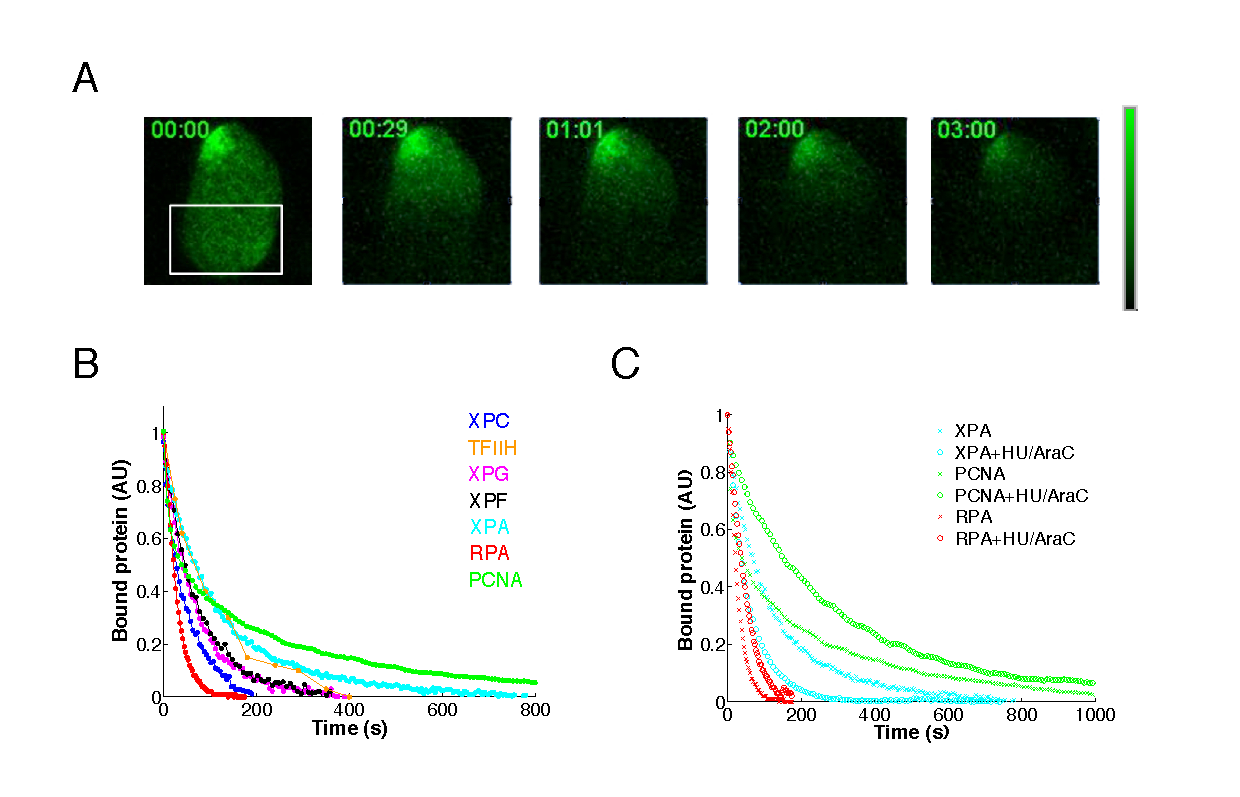
\includegraphics[width=1\textwidth]{Abbildungen/figure2_2_2.pdf}
  		\caption{\textbf{Rapid dissociation of NER factors from damaged DNA.} A) FLIP experiment in XP2OS cells stably expressing eGFP-XPA after 2 h of local irradiation. The nucleus is continuously bleached in an undamaged region (white rectangle). Fluorescence loss is recorded at the sites of local UV-irradiation B)\,Amount of bound NER-factors (XPC-eGFP, TFIIH-eGFP, XPG-eGFP, XPF-GFP, eGFP-XPA, RPA-eGFP and eGFP-PCNA) monitored over time at LD. C) Quantification of FLIP experiments in the absence or presence of HU and AraC for stably expressed eGFP-XPA, RPA-eGFP and eGFP-PCNA.}
  		\label{fig:accuFlip}
  	\end{center}
  \end{figure}



\section{Direct measurement of DNA resynthesis}
\label{Subsec:EdUmeasurement}

In order to expand our quantitative inspection of the NER pathway in intact mammalian cells, we established a protocol for the direct measurement of the repair synthesis process \cite{Verbruggen2014}. DNA resynthesis reflects the kinetics of the post-incision repair process, complementing the measurement of DNA lesion removal, which captures the system's behaviour of the pre-incision steps (cf.\ section \ref{sec:NERexperiments}). To mark newly-incorporated DNA shortly before and after local UV irradiation, cells were incubated in microscopy medium supplemented with 10 \textmu M 5-ethynyl-2'-deoxyuridine (EdU). Due to its excessive presence in solution, the DNA polymerase integrates EdU (a thymidine analogue) instead of the endogenous thymine into the new DNA strand (cf.\ Figure \ref{fig:EdU_measurement}A). After incubation for the desired time, cells were fixed, stopping EdU incorporation, and subsequently permeabilized. EdU was then tagged with the fluorescent azide (AlexaFluor-555, Life Technologies) forming a covalent bond by click chemistry \cite{Limsirichaikul2009}. Analogous to the quantification of NER factor dynamics, EdU intensities were captured with a laser scanning microscope (Zeiss).\\
\begin{figure}[b!]
	\begin{center}
		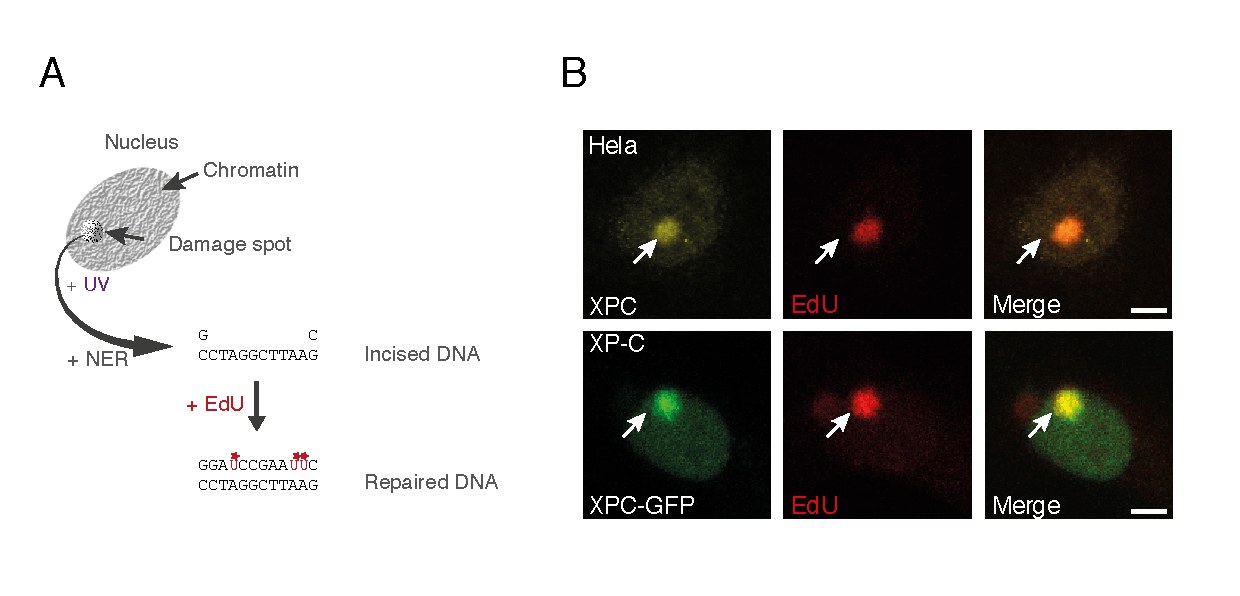
\includegraphics[width=1\textwidth]{Abbildungen/figure2_3.pdf}
		\caption{\textbf{EdU is incorporated at sites of local DNA damage.} A) Schematic illustration depicting the experimental procedure of EdU incorporation at sites of local damage. B) Antibody-stained endogenous XPC in Hela cells (upper panel) or stably expressed XPC-eGFP in XP-C cells (lower panel) accumulate in the LD spot and co-localize with incorporated EdU.}
		\label{fig:EdU_measurement}
	\end{center}
\end{figure}
\noindent Accordingly, incorporated EdU is exclusively present at the locally confined area of damaged and thereupon resynthesized DNA, which coincides with the localization of immunostained XPC (cf.\ Figure \ref{fig:EdU_measurement}B, upper row). The same result occurs for XP-C cells with stably-transfected XPC-eGFP (cf.\ Figure \ref{fig:EdU_measurement}B, lower row). Replicating cells could be excluded from the analysis due to the prevalent EdU incorporation distributed over the entire nucleus. 
  

    
 





\section{Repair rate follows first order rate kinetics}
\label{firstOrderRateKinetic}
In contrast to the real-time measurements for accumulation and dissociation of the NER factors, the incorporation of EdU cannot be followed continuously. As mentioned in section \ref{Subsec:EdUmeasurement}, cells have to be fixed and permeabilized before the newly incorporated bases can be fluorescently labelled. Therefore, only the accumulated EdU incorporated in the time interval between UV-irradiation and fixation can be followed. By repeating this procedure for growing time intervals we acquired successively the repair kinetics for newly-repaired DNA (cf.\ Figure \ref{fig:DNArepairKinetic}A and B). The signal at each time point represents the EdU signal averaged over multiple cells. \\
We found that EdU incorporation essentially stops after 4 hours, which coincides with the removal of 6-4PP (cf.\ \cite{Luijsterburg2010} and Figure \ref{fig:DNArepairKinetic}B). This agrees with the observation that NER is not primarily engaged in the removal of cyclobutane pyrimidine dimers (CPD) which are repaired on a much longer time scale \cite{Luijsterburg2010}. To test whether the availability of EdU is rate limiting, we measured the incorporation of EdU in discrete equidistant time intervals after UV-irradiation (cf.\ Figure \ref{fig:DNArepairKinetic}C). We observed that the amount of EdU incorporation per time interval (EdU rate) is indeed continuously declining and hence, the rate of repair synthesis. Moreover the EdU kinetic follows the trajectory of PCNA accumulation as measured by Luijsterburg \textit{et al.} \cite{Luijsterburg2010} (cf.\ Figure \ref{fig:DNArepairKinetic}D). PCNA is thought to act as processivity factor for the DNA polymerase and remains bound to the DNA \cite{Luijsterburg2010,Essers2005,Sporbert2002}. Taken together, these data establish EdU incorporation as a direct and quantitative measure for DNA repair synthesis in locally damaged nuclei.\\
The DNA repair time series characterized by incorporated EdU is fitted by a mono-exponential kinetic (cf.\ Figure \ref{fig:DNArepairKinetic}E):
\begin{equation}
EdU(t) = EdU_\text{max}(1 - e^{\lambda t}),
\label{Eqn:EdU_kinetic}
\end{equation}  
where $EdU(t)$ and $EdU_{\text{max}}$ give the amount of incorporated EdU and its value at saturation, respectively. The time constant was determined as $\lambda$=0.58 ($\pm$0.07) $\text{h}^{-\text{1}}$ using the polyfit function (pre-implemented in MATLAB). This result indicates that despite its molecular complexity, 6-4PP removal by NER is a slow first-order reaction with a half-time of 1.2 hours. \\
        
\begin{figure}[b!]
\begin{center}
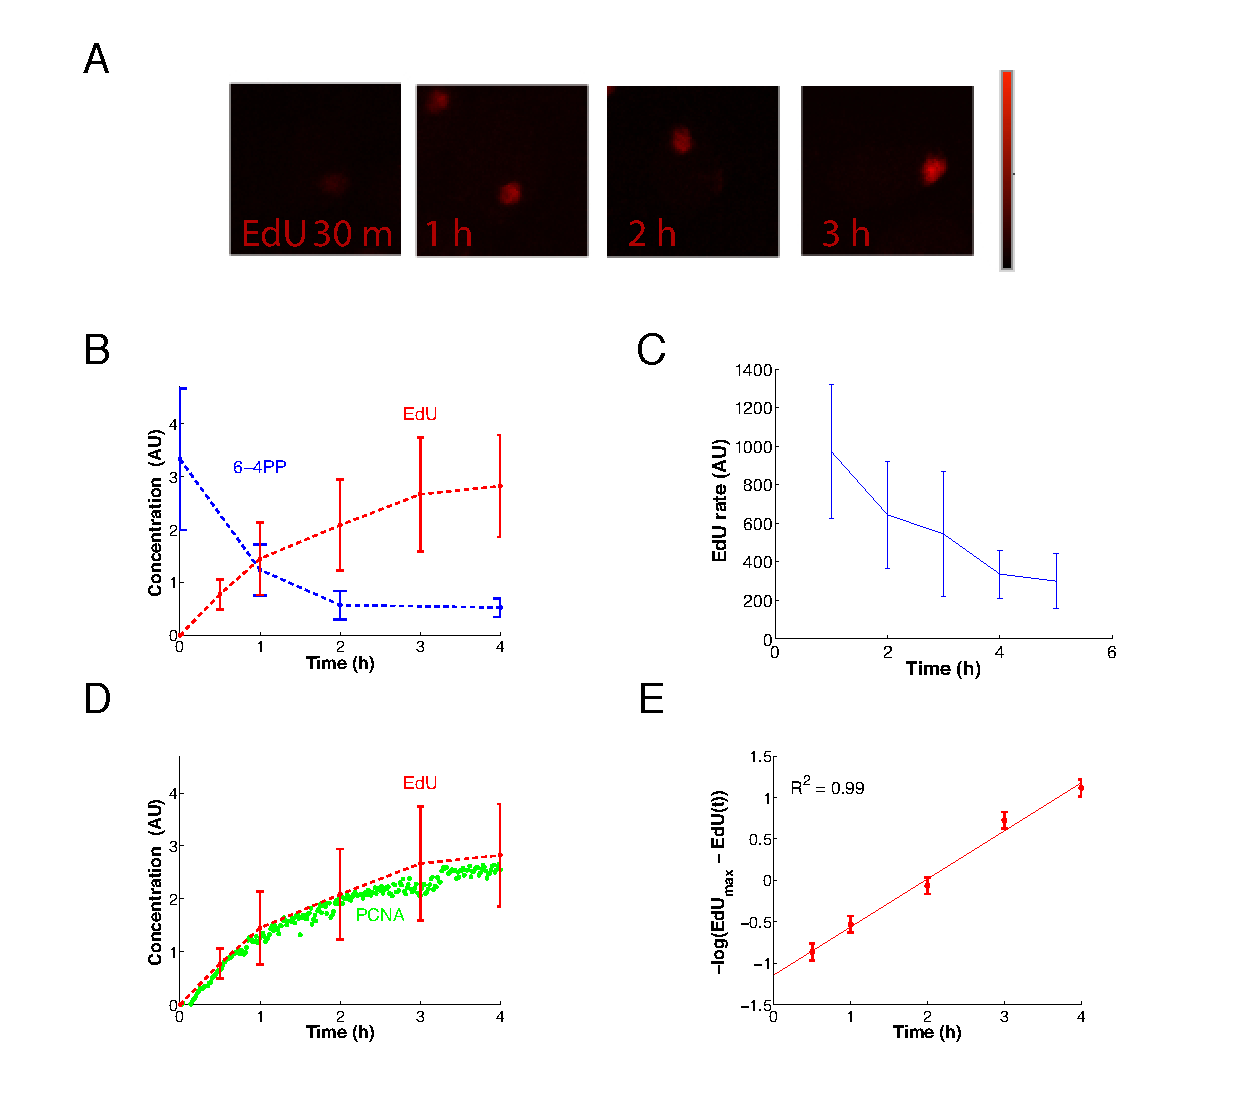
\includegraphics[width=1\textwidth]{Abbildungen/figure2_4.pdf}
\caption{\textbf{EdU incorporation reflects DNA repair synthesis quantitatively.} A) EdU signal at various time points after local UV-C irradiation. B) Repair DNA synthesis (EdU, red curve) coincides with damage removal (6-4PP, blue curve) measured previously by Luijsterburg \textit{et al.} (2010) \cite{Luijsterburg2010}. The EdU trajectory represents mean $\pm$\,SD (derived from three independent experiments) of DNA repair in locally damaged cells (n=150) per time point. C) Irradiated XP-C XPC-eGFP cells were treated with EdU for different time intervals post-irradiation. Intervals were chosen as follows: 15 minutes pre-irradiation to 60 minutes post-irradiation, 45-120 minutes, 105-180 minutes, 165-240 minutes and 225-300 minutes. Line plot represents mean $\pm$\,SD of EdU distributions derived from a particular time interval. D) DNA repair synthesis follows PCNA accumulation as measured previously \cite{Luijsterburg2010}. E) Mono-exponential fit of the EdU kinetic according to Eqn.\ \ref{Eqn:EdU_kinetic}.}
\label{fig:DNArepairKinetic}
% * <l.adlung@dkfz.de> 2014-12-07T10:08:06.916Z:
%
%  Explain UV-C in contrast to UV. Give R^2 for E
%
\end{center}
\end{figure}
Taken together, our experimental insight of the NER process got extended by following the kinetics of a repair intermediate directly. Now we are able to integrate our knowledge about the dynamic behaviour of individual repair factors and study its association with the overall repair rate quantitatively.    

%\clearpage{\pagestyle{empty}\cleardoublepage}

% ************************* PART III *****************************
\chapter{Kinetic model of NER}
\label{chap:kineticNERmodel}

Luijsterburg \textit{et al.} developed a mathematical NER model by integrating a large data set for all seven core NER factors \cite{Luijsterburg2010}. However, despite the comprehensive collection of time-resolved \textit{in vivo} measurements of the individual protein dynamics the model parameters comprising binding, dissociation and catalytic constants were not fully identified by the data. This is presumably caused by the missing readout of DNA repair, which was so far not measured on a similar time-scale as the protein assembly rates and the dwell times. Unfortunately, the non-identifiability sets a limitation for the predictive power of the model. \\ 
Based on the EdU incorporation data introduced in chapter \ref{chap:quantData} we present here an evolved mathematical model of NER. It explains the connection between the dynamic exchange of individual repair factors at damaged chromatin sites and the overall time scale of the entire repair process. We calibrated the parametrization of the model iteratively with a profile likelihood estimation leading to identifiable parameters and hence an increased predictive power of the model. As a consequence, our fully identifiable model can reliably predict the behaviour of the experimentally inaccessible repair intermediate of incised DNA.\\
   



\section{Slow first-order reaction kinetic due to many fast interacting components}
\label{sec:toyModel}
To investigate the mechanistic connection between fast NER factor exchange at the DNA template and the overall slow repair time, it appears practical to apply an analytical approach. During her Ph.D. thesis, Dr.\ Gesa Terstiege supervised by Prof.\ Thomas H\"ofer performed this analysis \cite{Terstiege2010,Verbruggen2014}, considering the complex formation with a simplified model of repair including $N$ repair factors. They examined different scenarios distinguishing between random and sequential protein assembly; reversible and irreversible protein binding, or mixed mechanisms specific for each DNA repair intermediate (cf.\ Figure \ref{fig:reactionTiming}A,\cite{Verbruggen2014}). Under appropriate assumptions, the mean repair time of such a process can be generally described with:

\begin{equation}
\tau = \underbrace{\frac{1}{k}\sum^{N-1}_{i=0}K_i\left(\frac{l}{k}\right)^i}_{\text{first assembly}} +  \underbrace{\frac{1}{\rho}\sum_{i=0}^{N}J_i \left(\frac{l}{k}\right)^i}_{\text{reassembly and reaction}}, \label{Eqn:taugen}
\end{equation}

where $k$ denotes the pseudo first-order association rate constant of NER factors, $l$ the dissociation rate constant of NER factors and $\rho$ the rate of the repair reaction. $K_i$ and $J_i$ differ between random assembly
\begin{equation}
K_i^\text{rand}= \sum_{j=1}^{N-i}\frac{1}{i+j}\frac{{N \choose j-1}}{{N\choose i+j}} , \quad J_i^\text{rand} = {N\choose i}\label{Eqn:coefrand}
\end{equation} 
and sequential assembly           
\begin{equation}
K_i^\text{seq}= N-i , \quad J_i^\text{seq} = 1.\label{Eqn.coefseq}
\end{equation}
Considering reversible protein binding ($l=k=1$), sequential and random assembly occur on a similar time scale for fewer than or equal to 10 components \cite{Terstiege2010}, which coincides with the number of core NER factors \cite{Luijsterburg2010}. The theoretical component number where both assembly strategies have a similar timing is even higher for increasing reaction rates ($\rho \gg k,l$). Given that all repair factor dwell times are in the order of $\sim$1 min ($k$ = $l$ = 1 $\text{min}^{-\text{1}}$), the model was simulated for $N$ = 9 components. The resulting trajectory followed a single-exponential kinetic with a half-time of $\sim$1 hour in the case of balanced reversibility. In contrast, for an irreversible process ($l/k = 0$) the repair kinetic resembles a sigmoid time course (cf.\ Figure \ref{fig:reactionTiming}B). These results suggest that the rapidly exchanging NER factors naturally generate a mono-exponential repair kinetic, whereas the slow overall time span can be explained by the stochastic distribution of repair events. This leads to a large number of non-functional repair complexes before the catalytically active complex is assembled.  


\begin{figure}[t]
\begin{center}
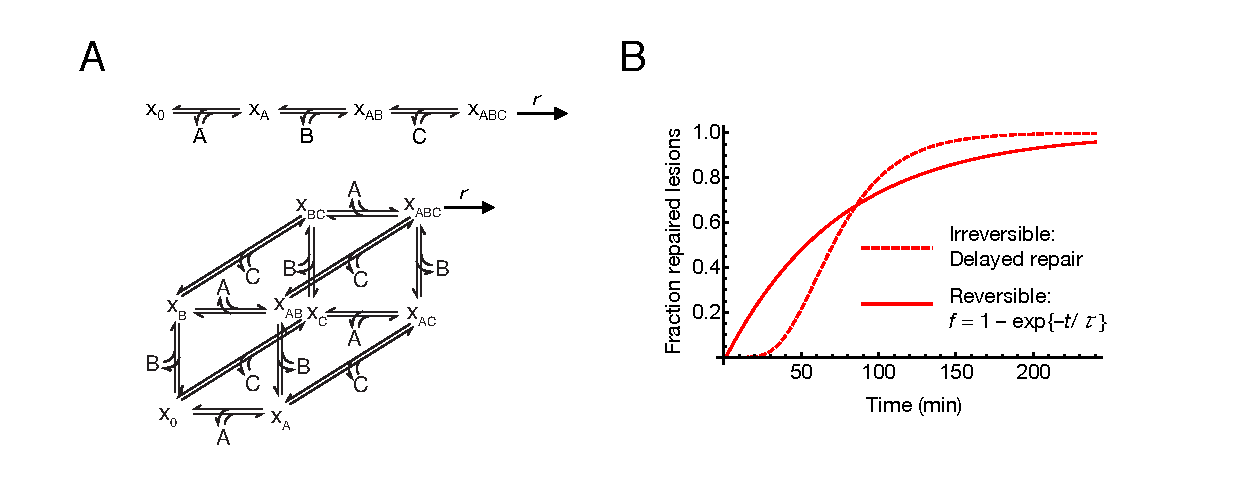
\includegraphics[width=1\textwidth]{Abbildungen/figure2_5_2.pdf}
\caption{\textbf{Simplified analytical model of the repair complex formation.} A) Sequential (upper panel) and random (lower panel) assembly scheme of the repair factors A, B and C to the DNA template $\text{x}_i$, $i \in \{\text{A, B, C, AB, AC, BC, ABC}\}$. $\text{x}_0$ denotes the empty lesion (e.g. damaged DNA). When the complex is fully assembled ($\text{x}_{\text{ABC}}$) it performs a catalytic repair step with rate $r$. B) Simulated repair time courses for random reversible (solid line) and irreversible (dashed line) repair factor assembly. For reversible binding ($k=l= \text{1 min}^{-1}, N=\text{9}$) the trajectory fits a mono-exponential repair kinetic with time constant $\tau$, whereas for irreversible binding the fit has sigmoidal shape ($l=\text{0}, k=\text{0.037 min}^{-1}, N=\text{9}$, chosen to get the same time constant).}
\label{fig:reactionTiming}
\end{center}
\end{figure}


\section{Model structure and parametrization}
To examine the relation between rapid repair factor exchange and the slow first-order reaction kinetic, we extended the previously performed analysis \cite{Luijsterburg2010,Terstiege2010}, by considering a more realistic NER model. Conceptually, the model developed here, follows on the model introduced by Luijsterburg \textit{et al.} (2010) \cite{Luijsterburg2010}. In their model NER factors bind transiently to DNA repair intermediates to form catalytic complexes that, if complete, perform the next repair step. The latter are usually irreversible reactions embodying the sequential characteristics of this pathway (cf.\ Figure \ref{fig:introScheme}A).\\
The nature of these distinguishable repair intermediates has been widely investigated \textit{in vitro} and \textit{in vivo} \cite{Evans1997a,Mu1996,Polo2006,Tapias2004}.
The evolved model, presented here, distinguishes five DNA repair intermediates: damaged DNA, unwound DNA, incised DNA, resynthesised DNA and rechromatinised DNA. The molecular state of these intermediates defines the binding affinity for a specific set of repair proteins (cf.\ Figure \ref{fig:ModelStructure}). Table \ref{tab:modelassumptions} summarizes all repair intermediates and lists the corresponding repair factors that show affinity for a particular repair intermediate. Repair factors that catalyse the enzymatic reaction if assembled are indicated. As stated before, FLIP measurements indicated that diffusion is not rate limiting for protein binding and therefore, we do not include it in the model (cf.\ Section \ref{subsec:AccuFlipExp} and \cite{Rademakers2003,Zotter2006}).              


\begin{figure}[b!]
\begin{center}
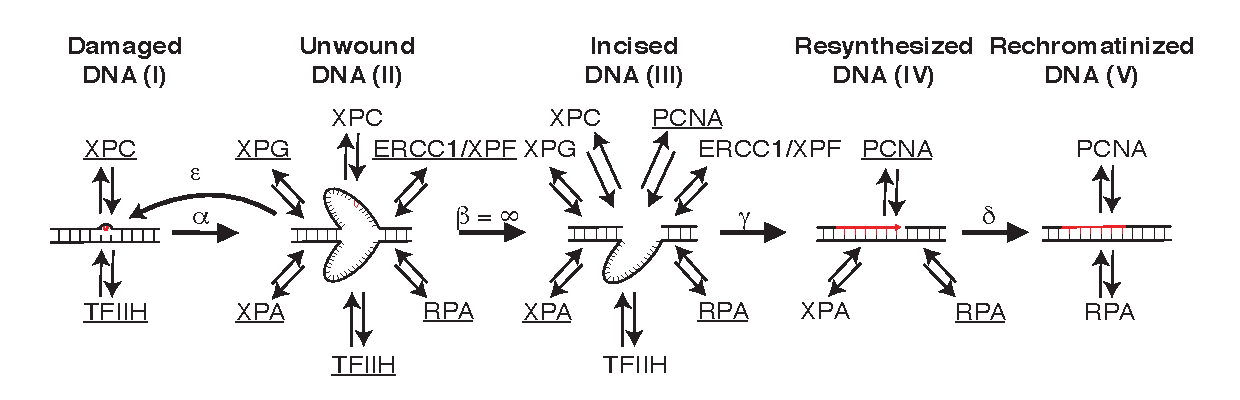
\includegraphics[width=1\textwidth]{Abbildungen/figure2_5.pdf}
\caption{\textbf{Schematic model description of the DNA repair mechanism.} The model distinguishes five individual repair intermediates: Damaged (I), unwound (II), incised (III), resynthesised (IV) and rechromatinised DNA (V). As indicated, specific tuples of repair proteins bind reversibly to the intermediates. Catalytic reactions, denoted by Greek letters, occur when the catalytic reaction complex (underlined proteins) is assembled.}
\label{fig:ModelStructure}
\end{center}
\end{figure}


Theoretical results suggest that the detection of damaged DNA sites by a single element instead of multiple elements simultaneously is crucial for the efficient initiation of the repair process \cite{Politi2005,Volker2001}. This prominent role within the NER pathway plays the lesion recognition factor XPC. Besides this experimentally verified exception, we assumed random and non-cooperative binding for all NER factors.\\ 
\begin{table}[t!]
	\small{
		\begin{tabular}{cccccc}
			\hline
			\rule{0pt}{2ex}
			\textbf{Repair}&\textbf{Binding} &	\textbf{Catalysed  process}&\textbf{Remarks}  	&\textbf{Ref.} \\ 
			\textbf{intermediate}&	\textbf{proteins} &	\textbf{Required proteins}&	& \\ \hline
			\rule{0pt}{3ex}
			(I) Damaged DNA&	XPC,TFIIH 	&Unwinding &Initiation by binding	&\cite{Evans1997a}
			\\ 
			&	(3 states)& (reaction $\alpha$)&  of XPC and subsequent &\cite{Riedl2003}\\
			&&XPC and TFIIH&	 recruitment of TFIIH. &\cite{Yokoi:2000:J-Biol-Chem:10734143}\\ 
			&&&&\cite{Rademakers2003}\\ 
			&&&& \cite{Volker2001} \\ 
			&&&&\\\hline
			\rule{0pt}{3ex}
			(II) Unwound DNA&XPC,TFIIH,&Dual incision &If the DNA becomes &\cite{Evans1997a} \\
			& XPG, XPA,&(reaction $\beta$)&devoid of any protein,&\cite{ODonovan:1994:Nature:8090225}\\
			&ERCC1/XPF,&TFIIH,XPG,&it will re-anneal (reaction &\cite{Sijbers:1996:Cell:8797827}\\
			&  RPA& XPA,  RPA&$\varepsilon$). Dual incision requires&\cite{Winkler2001}\\
			&(64 states)&and ERCC1/XPF&the endonucleases XPG& \cite{deLaat:1998:Genes-Dev:9716411}\\
			&&&  and ERCC1/XPF and is&\\
			&&&stimulated by TFIIH, &\\
			&&&XPA, RPA and possibly &\\
			&&&XPC.&\\
			&&&& \\ \hline
			\rule{0pt}{3ex}
			(III) Incised&XPC,TFIIH,&Repair-synthesis&PCNA binds to the free&\cite{Evans1997a}\\
			DNA& XPG, XPA,& (reaction $\gamma$)&3'-OH group generated by&\cite{Winkler2001}\\
			& ERCC1/XPF,&XPA, RPA and&  the ERCC1/XPF incision.&\\
			&RPA, PCNA& PCNA& DNA polymerase is also&\\
			&(128 states)&& required (not measured).	&\\
			&&&& \\   \hline
			\rule{0pt}{3ex}
			(IV) Resynthesised&XPA, RPA,&Rechroma-&Accumulation&\cite{Moser2005}\\
			DNA&	 PCNA& tinization& data imply that XPA&  \cite{Shivji:1995:Biochemistry:7711023}\\
			&(8 states)&(reaction $\delta$)& binds  to repaired DNA &\cite{Luijsterburg2010}\\
			&&RPA and PCNA&while the pre-incision &\\
			&&&	  proteins do not &\\
			&&& (Figure \ref{fig:accuImage}C).&\\
			&&&& \\ \hline
			\rule{0pt}{3ex}
			(V) Rechromatin- &RPA, PCNA &&RPA and PCNA associate&\cite{Riedl2003}\\
			ised DNA &(4 states)	&&with repaired intermediate $I$,&\cite{Luijsterburg2010}\\
			&&&as levels of bound eGFP-&\\
			&&&PCNA and eGFP-RPA&\\ 
			&&& are  high up to at least 4 h&\\
			&&& after UV irradiation, while&\\
			&&& other repair proteins are&\\   
			&&& no longer bound.&\\   &&&& \\ \hline
		\end{tabular}}
		\caption{\textbf{Model assumptions.} Adapted from Terstiege \textit{et al.} (2010) \cite{Terstiege2010}}\label{tab:modelassumptions}
	\end{table}
	\newpage
	\cleardoublepage  
	 
The model structure introduced above and shown in Figure \ref{fig:ModelStructure} was translated into an ordinary differential equation system assuming mass-action kinetics for all protein-DNA interaction processes. Each equation describes the concentration of a single DNA state $y_{\pi}^{R}$ (cf.\ Eqn. \ref{eqn:DNAstatesModel}) associated with a specific repair intermediate $R$ = I, II,\dots,V (damaged (I), unwound (II), incised (III), resynthesised (IV), rechromatinised (V)). The index $\pi$ represents a binary vector, where each position displays the presence or absence of a repair protein $p$ ($p$ $\in$ {C, T, G, A, F, R, P}, where XPC (C), TFIIH (T), XPG (G), XPA (A), ERCC1/XPF (F), RPA (R) and PCNA (P)). $\pi(p)=1$ if protein p is bound and $\pi(p)=0$ if not. The length of $\pi(p)$ is defined according to the model structure (cf.\ Table \ref{tab:modelassumptions}) with: $\pi_{R=I} = \{ \text{C,T} \}$; $\pi_{R=II} = \{ \text{C,T,G,A,F,R} \}$; $\pi_{R=III} = \{ \text{C,T,G,A,F,R,P} \}$; $\pi_{R=IV} = \{ \text{A,R,P} \}$; $\pi_{R=V} = \{ \text{R,P} \}$. The time course of this model is described by

\begin{equation}\label{eqn:DNAstatesModel}
\frac{d}{dt}\;y_{\pi}^{R} =\sum_{p\text{ in }R}\eta \, \left( (-1)^{\pi(p)} \,l_{p}^{ R}\, y_{\pi}^{R}\left. \right|_{\pi(p)=1}+  \, (-1)^{1+\pi(p)}\, k_{p}^{ R} \,C_p(t)\,y_{\pi}^{R}\left. \right|_{\pi(p)=0}\right ) +E(y_{\pi}^{R}),
\end{equation}\\
where $\eta$ represents a cooperativity ensuring the inclusion of all cooperative binding events:

\begin{align*}
\eta =\left\{
\begin{array}{llll}
& 0 \quad   &\text{if}& R=\text{I} ~\wedge~ p=\text{C} ~\wedge~ \text{T}=1, \\
&     && R=\text{I} ~\wedge~ p=\text{T} ~\wedge~ \text{C}=0,\\
& 1 \quad &\text{otherwise}.&
\end{array}
\right.
\end{align*}
  
The kinetics describing protein exchange at the repair intermediates are characterized by the binding $k_{p}^{ R}$ and dissociation constants $l_{p}^{ R}$, respectively. The free protein concentrations are denoted by $C_p(t)$ representing seven additional ordinary differential equations for $p \in \{\text{C,T,G,A,F,R,P}\}$:

\begin{eqnarray}\label{Eqn:concentration}
\frac{d}{dt}\;C_p&=&\,\sum_{R=\text{I}}^{\text{V}} \sum_{\pi} \xi \left( \,\delta_{\pi (p)1}\;l_{p}^{ R}\, y_{\pi}^{R}- \,\delta_{\pi (p)0}\; k_{p}^{ R} \,C_p\,y_{\pi}^{R}\right)
\end{eqnarray}  

Analogous to $\eta$, $\xi$ governs the sequential binding of XPC and TFIIH by:

\begin{align*}
\xi =\left\{
\begin{array}{l l ll}
& 0 \quad   &\text{if} & R=\text{I} ~\wedge~ \text{C}=0 ~\wedge~ \text{T}=1, \\
&    && R=\text{I} ~\wedge~ p=\text{C} ~\wedge~ \text{C}=\text{T}=1, \\
&    &&R=\text{I} ~\wedge~ p=\text{T} ~\wedge~ \text{C}=\text{T}=0, \\
& 1 \quad& \text{otherwise}.&
\end{array}
\right.
\end{align*}

The Kronecker delta 
 \begin{align*}
\delta_{ij}=\left\{
\begin{array}{l l l l}
&1 \quad   &\text{if} & i=j\\
&0 \quad& \text{if } & i \neq j\\
\end{array}
\right.
\end{align*}
ensures that a protein only binds to complexes, where it is yet missing and only leaves complexes, where it is actually present.\\
Finally, when an enzymatic complex has fully assembled at the DNA template, it catalyses the next repair step, which is represented in the model by the term $E(y_{\pi}^{R})$ in Eqn.\ \ref{eqn:DNAstatesModel}. After damage recognition by XPC, damaged DNA is unwound by the helicase TFIIH with the unwinding activity $\alpha$, whereas XPC acts as a stabilizing/proof-reading factor in parallel. Accordingly, $E(y_{\pi}^{R})$ translates into the following catalytic reactions for damaged DNA ($R= \text{I}$):
$$E(y_{00}^\text{I})=\;\varepsilon\;y_{000000}^\text{II} \quad \text{ and }\quad
E(y_{11}^\text{I})=\;-\alpha \;y_{11}^\text{I}.$$
If all proteins fall off the DNA template due to false damage detection, the DNA will re-anneal with the rate $\epsilon$. Otherwise a complex formed by TFIIH, XPG, XPA, XPF and RPA will eventually promote the excision of the lesion DNA strand leading to the following catalytic reactions for unwound DNA ($R= \text{II}$): 	
\begin{align*}
	\begin{array}{l l l}
		E(y_{000000}^\text{II})&=&-\;	\varepsilon	\;y_{000000}^\text{II}\;, \\ E(y_{110000}^\text{II})&=&\;	\alpha	\;y_{11}^\text{I} 	\text{ and }\\
	    E(y_{011111}^\text{II})&=&-\	\beta	\;y_{011111}^\text{II}.
	\end{array}
\end{align*}

Once the lesion strand is excised with incision rate $\beta$, the remaining repair steps are irreversible. Incised DNA is resynthesised with the rate $\gamma$ by the resynthesis complex  XPA-RPA-PCNA. XPA is assumed to assemble at post-incision repair intermediates as suggested by experiments with inhibited incision that showed accelerated dissociation FLIP kinetics for XPA  \cite{Luijsterburg2010}. This result is supported by a chromatin immunoprecipitation (ChIP) experiment with antibodies against XRCC1-Lig III showing the co-precipitation of XPA and RPA but not XPC and TFIIH \cite{Moser:2007:Mol-Cell:17643379}. Evidence for the importance of PCNA and RPA for the resynthesis reaction was shown by Shivji \textit{et al.} (1995) \cite{Shivji:1995:Biochemistry:7711023}, and therefore we incorporate the following catalytic reactions for incised DNA ($R= \text{III}$):  
            
\begin{align*}
\begin{array}{l l llll}
E(y_{1111111}^\text{III})&=&\;	\beta \;	y_{011111}^\text{II}	 \quad \text{and}
&E(y_{0001011}^\text{III})=&\;	-\gamma	\;y_{0001011}^\text{III}.	 \\
\end{array}
\end{align*}

In correspondence to the previously described accumulation measurements (cf.\ Figure \ref{fig:accuImage}), only RPA and PCNA stay bound during chromatin remodelling (the last modelled repair intermediate). This leads to the following enzymatic reactions for resynthesised DNA  ($R= \text{IV}$) and rechromatinised DNA ($R= \text{IV}$):


\begin{align*}
\begin{array}{l l llll}
E(y_{111}^\text{IV})&=&\;	\gamma \;	y_{0001011}^\text{III},\\	 
E(y_{011}^\text{IV})&=&\;	-\delta	\;y_{011}^\text{IV} \text{ and }	 \\
 E(y_{11}^\text{V})&=&\;	\delta	\;y_{011}^\text{IV}.
\end{array}
\end{align*}

Due to the non-cooperativity assumption of all NER factors, there are a total of $2^N$ repair states where $N$ denotes the number of repair proteins assembling to the particular repair intermediate. The only exception is the sequential assembly of TFIIH, after lesion detection by XPC, which reduces the number of states for damaged DNA to $ 2^2-1 = 3$ states. For the remaining repair intermediates we derive  $ 2^6 = 64$ states for unwound DNA; $ 2^7 = 128$ states for incised DNA; $ 2^3 = 8$ states for resynthesised DNA and $ 2^2 = 4$ states for rechromatinised DNA. This results in a total of 214 states including seven differential equations for the free NER-factor protein concentrations. \\
Summing over all repair states and the respective intermediates associated to one repair factor, we can simulate its accumulation kinetic. The initial conditions are the measured free protein concentrations denoted in Table \ref{tab:nuclearconcentrations}\cite{Terstiege2010,Luijsterburg2010} and the initial amount of inflicted damages was estimated with  $y_{00}^{\text{I}} = 3.33$ \textmu M \cite{Verbruggen2014}. The remaining initial states were assumed to be zero. To reproduce the FLIP kinetic for a specific repair factor, all corresponding dissociation constants were set to zero when the FLIP experiment started (at the time where protein accumulation at LD reached the plateau level). Accordingly, FLIP kinetics were acquired after 600 s for XPC and ERCCC1/XPF, 900 s for XPG and TFIIH, 2000 s for XPA and 7200 s for PCNA. 


 

\section{A maximum likelihood approach for efficient model fitting}
\label{sec:maximumLL}
To find a realistic parametrisation for the temporal development of the repair states $y_\pi^R$ (cf.\ Eqn.\ \ref{eqn:DNAstatesModel}) the model was mapped to $m$ observables $z_k$ via the function $f_{z_k}$:

  \begin{equation}
  	z_k(t_i,\theta) = f_{z_k}(t_i,y(t_i,\theta),\theta).
  	\label{eqn:observable}
  \end{equation} 

The observables $z_k$ are parametrised by $\theta$ and resemble experimentally-derived quantities at time $t_i$. $\theta$ depicts binding, dissociation and catalytic constants. Each model observable $z_k(t_i,\theta)$ corresponds to the measured data $z_k^\dag(t_i)$ with intrinsic noise $\epsilon_{ki}$. The data is usually the sum of measurement noise combined with the naturally occurring biological variability. Assuming additive, normally distributed noise leads to $z_k^\dag(t_i) = z_k(t_i,\theta) + \epsilon_{ki}$ with $\epsilon_{ki} \sim N(0,\sigma_{ki}^2)$. To calibrate the measured data $z_k^\dag(t_i)$ with the model observables $z_k(t_i,\theta)+\epsilon_{ki}$, we applied a maximum likelihood approach as distance measure which translates, considering normally distributed noise, into:
\begin{equation}
\label{eqn:likelihood}
L(z_k^\dag \textbar \theta) = \prod_{k=1}^m \prod_{i=1}^{d_k} \frac{1}{\sqrt{2\pi \sigma_{ki}^2}}\exp \left( -\frac{1}{2\sigma_{ki}^2}\left(z_{ki}^\dag(t_i) - z_k(t_i,\theta)\right)^2\right).
\end{equation}
  
Here, $d_k$ denotes the number of distinct experimental data-sets ($t_i,z_k^\dag$) for each measured observable $k = 1,\ldots,m$, measured at time points $t_i$ with $i = 1,\ldots,d_k$. $\sigma_{ki}^2$ are the variance components of the measurement noise of each data point. Instead of maximizing the likelihood it is equivalent and numerically more efficient to minimize its negative logarithm multiplied with 2: $-2\log(L(z_k^\dag\textbar\theta))$, which we will refer to in the following as $X^2$.  

\begin{equation}\label{eqn:chiSquare}
X_\theta^2 = -2\log(L(z_k^\dag\textbar\theta)).
\end{equation}

For the minimization of $X^2$ the choice for $\theta$ is controlled by $\sigma_{ki}^2$ (cf.\ Eqn.\ \ref{eqn:likelihood}). As shown by Raue and colleagues \cite{Raue2013}, for a reliable estimation of the model parameters $\theta$, the simultaneous approximation of $\sigma_{ki}^2$ together with the model dynamics leads to a statistically more accurate assessment of the model parameters than using noise estimations from preprocessed data \cite{Raue2013}. Accordingly $\sigma_{ki}^2$ can be considered as parametrised function

\begin{equation}
\sigma_{k}(t_i,\theta) = f_{\sigma_{k}}(t_i,z_(t_i,\theta),\theta),
\end{equation}    

wherein additional parameters are introduced representing the type and magnitude of the modelled noise. Analogous we applied an additive error model for each observable with the parametrised function $\sigma_{k}(t_i,\theta) = s_a$ and $\epsilon_{ki} \sim N(0,\sigma_{ki}^2)$, where $s_a$ is included in $\theta$.\\ 
For reasons of fitting-speed efficiency we implemented our model into the online-available D2D software environment \cite{Raue2013} optimized for MATLAB (2011a, The Mathworks Inc., Natick, MA). The integrated fitting procedure applies the trust region algorithm LSQNONLIN, which is pre-implemented in MATLAB. The algorithm requires the derivatives of the objective function with respect to the parameters (cf.\ Eqn.\ \ref{eqn:likelihood}). The inner derivatives $dy(t,\theta)/d\theta$, also called sensitivities, provide gradient information about the parameter landscape and thus, are crucial to guide the optimization algorithm to the nearest optimum. The sensitivities can be passed into the form of sensitivity equations 

\begin{equation}
	\frac{d}{dt}\frac{dy(t,\theta)}{d\theta} = \frac{\partial f_y}{\partial y}\frac{dy(t,\theta)}{d\theta}+\frac{\partial f_y}{\partial \theta},
\end{equation}  

which represent additional ODEs that are solved in parallel to the original ODE system (cf.\ Eqn.\ \ref{eqn:DNAstatesModel} and Eqn.\ \ref{Eqn:concentration})\cite{Leis1988}. Applying sensitivity equations instead of a simple finite difference approximation proved to be numerically more accurate and computationally faster \cite{Raue2013}. Both, model and sensitivity ODEs were solved with the CVODES algorithm written in ANSI standard C \cite{Hindmarsh2005}. \\
To avoid terminating the optimization procedure in a local minimum we used a 'multi-start' approach by drawing the initial parameter vector using Latin hypercube sampling (LHS) \cite{Owen2014}. In contrast to a random sampling approach, LHS provides a better coverage of the sampling space by maximizing the distance between successive parameter drawings \cite{Raue2013}.    





\section{NER model fits accumulation, FLIP and repair synthesis measurements}    

To derive faithful fitting results we reiterated the optimization process 250 times. For each iteration the starting parameters were redrawn by Latin hypercube sampling. Despite the size of the model, with respect to data points and the number of parameters, the majority of fits terminated within one order of magnitude compared to the global $X^2$ minimum (cf.\ Figure \ref{fig:LHS}).
\begin{figure}[t]
	\begin{center}
		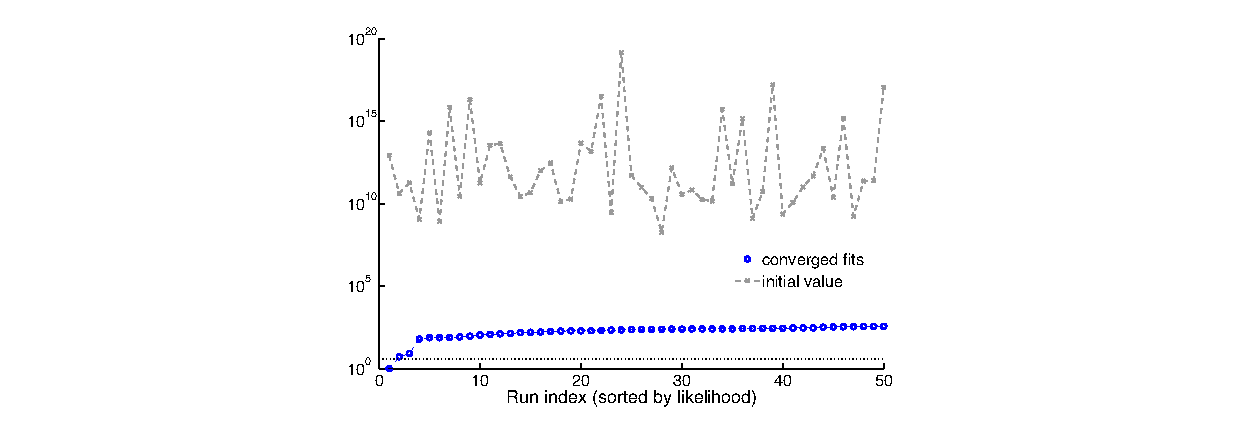
\includegraphics[width=1\textwidth]{Abbildungen/figure2_6_4.pdf}
		\caption{\textbf{Parameter estimation for the 50 best fits after initial Latin hypercube sampling.} Visualization of performance using the 50 (out of 250) best independent optimization runs (blue dots depict final optima of each individual run). Initial guesses (grey stars) were generated by Latin hypercube sampling. For illustrative purposes the global optimum is centred to 1.}
		\label{fig:LHS}
	\end{center}
\end{figure} 

Compared to the average initial $X^2$-value, the average fit improvement was about eight orders of magnitude. For the optimal parameter set, the model fits the experimental data comprising accumulation, FLIP, perturbation and repair synthesis measurements (cf.\ Figure \ref{fig:ModelFit_accu_flip}A, B, C; estimated measurement errors are shown as shaded area around the fit). The accumulation kinetics (cf.\ Figure \ref{fig:ModelFit_accu_flip}A) are depicted as concentrations scaled by the volume of the locally damaged area, which were estimated with 10\% of the nuclear volume (average derived from segmentation results of the nucleus and the LD foci). We believe that this specification is more intuitively comprehensible  compared to scaling by the whole nuclear volume as performed by Luijsterburg \textit{et al.}\cite{Luijsterburg2010}. It allows the realistic comparison between simulated and measured microscopy images of NER factor accumulation and EdU incorporation (cf.\ Figure \ref{fig:Fitt_accu_Mic}).  

\begin{figure}[htbp]
	\begin{center}
		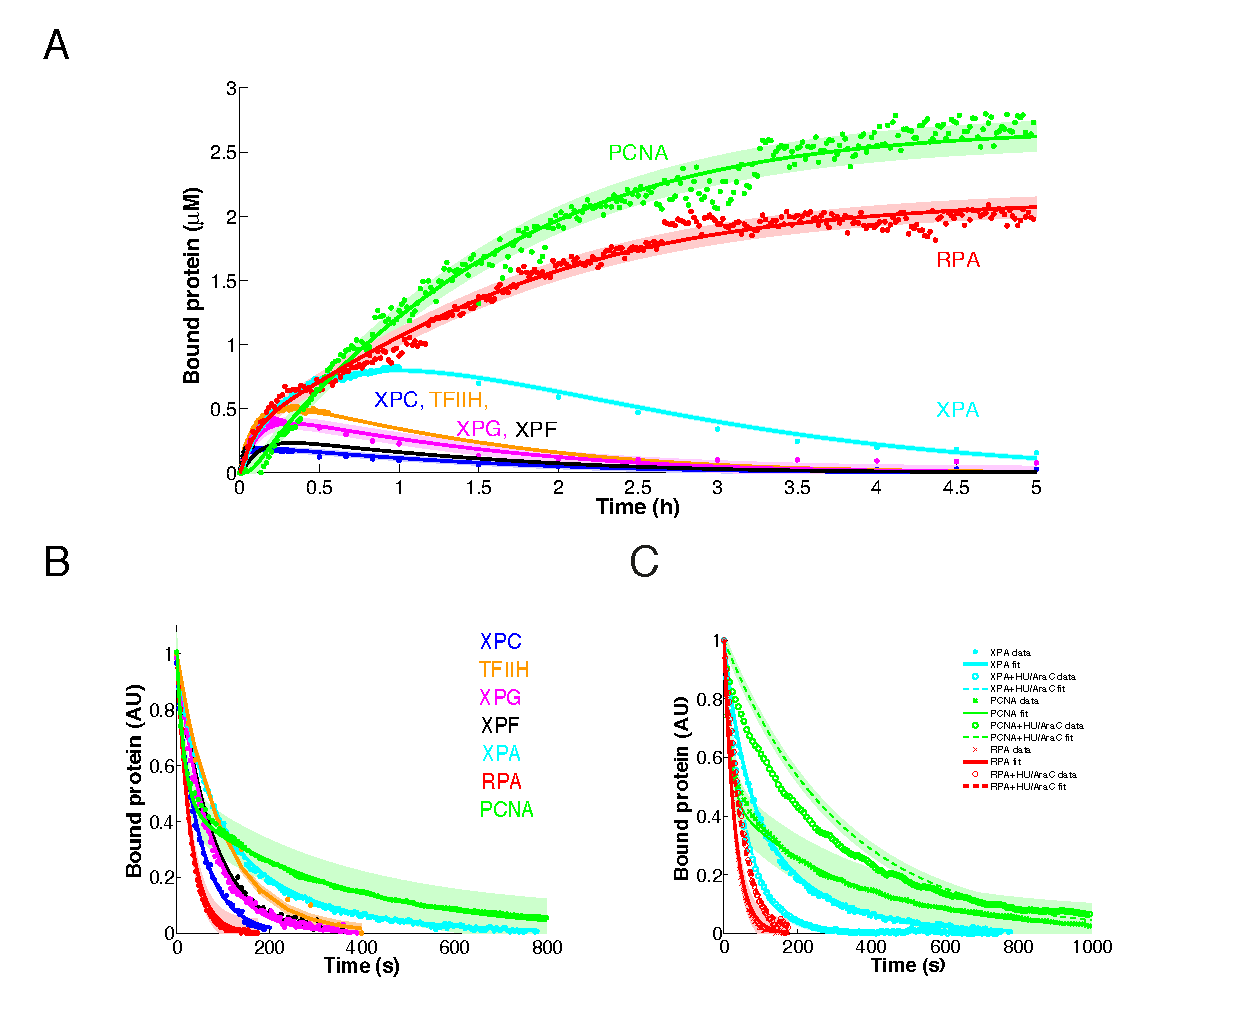
\includegraphics[width=1\textwidth]{Abbildungen/figure2_6.pdf}
		\caption{\textbf{Quantitative NER model fits to accumulation and dissociation time courses.} A) and B) Simulation (lines) and measurement (dots) of the accumulation and dissociation kinetics for the repair factors XPC, TFIIH, XPG, XPA, XPF, RPA and PCNA. Estimated errors are depicted as shaded area. C) Fitted FLIP time courses of XPA, RPA and PCNA in the absence or presence of AraC and HU on locally irradiated cells.}
		\label{fig:ModelFit_accu_flip}
	\end{center}
\end{figure}
\begin{figure}[t!]
\begin{center}
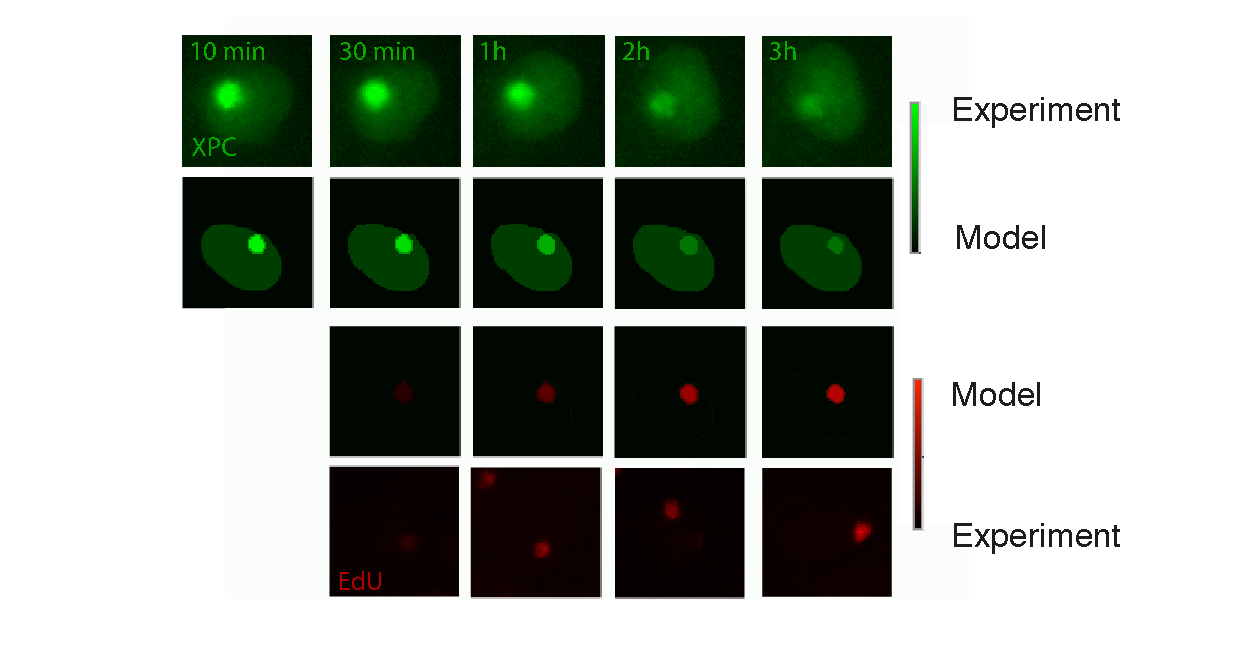
\includegraphics[width=1\textwidth]{Abbildungen/figure2_6_2.pdf}
\caption{\textbf{Comparison between measured and simulated single cell microscopy images.} Simulated time courses and the associated microscopy images for GFP tagged XPC (two upper rows) and EdU incorporation (two lower rows). Simulated XPC expression intensities were normalized to the nuclear intensities of the microscopy images. For the EdU incorporation intensities were scaled according to the highest and lowest intensity values of the microscopy images.}
\label{fig:Fitt_accu_Mic}
\end{center}
\end{figure}

\section{Profile likelihood analysis identifies realistic model of NER}
\label{sec:identifiabilityAnalysis}
In this section we quantify the quality of the model fit and determine whether the current model structure is competent for reliable predictions concerning experimentally unobserved system behaviour. This capability depends on the structural and practical identifiability of the model, which can be influenced by functionally related parameters or by the limited amount and quality of the data, respectively \cite{Cobelli1980,Swameye2003}. Both can be analysed and tested numerically by a formalism called profile likelihood estimation (PLE)\cite{Venzon1988,Murphy2000,Raue2009}, where the multi-dimensional model uncertainty inflicted by an individual parameter is projected to a one-dimensional profile likelihood (PL)
\begin{equation}
PL(\theta_i) = \max_{\forall j \neq i} [L(z_k^\dag \lvert \theta_j)].
\label{eqn:PL} 
\end{equation}
One parameter $\theta_l$ with $l\in\{{1,\ldots,N}\}$ at a time, is gradually fixed along this dimension for different values of $p$. In each step the negative log-likelihood $X_{\theta_l}^2(p)$ is minimized (cf.\ Eqn.\ \ref{eqn:chiSquare}), fitting all other parameters $\theta_k$ with $k\in\{{1,\ldots,N}\}$; $k\neq l$. Subsequently, the identifiability of a parameter $\theta_l$ can be determined by $\Delta X_{\theta_l}^2(p)$, which describes the difference between the parameter dependent local minimum $X_{\theta_l}^2(p)$ and the global $X^2$ minimum
\begin{eqnarray}
	\Delta X_{\theta_l}^2(p) &=& \min_{\{\theta_k\textbar k=1,\ldots,N;k\neq l\}} \left( X^2 (\theta_1,\ldots,\theta_{l-1},p,\theta_{l+1},\ldots,\theta_N )\right)\nonumber \\
	&-& \quad \! \min_{\{\theta_k\textbar k=1,\ldots,N\}} \quad \!\! \left( X^2 (\theta_1,\ldots,\theta_N )\right).
\end{eqnarray}  

Confidence bounds for the particular parameter depend on the threshold $Q_{X^2}(1-a,df)$, which represents the $(1-a)$ quantile of the $X^2$-distribution with $df$ degrees of freedom. The associated point-wise confidence intervals are defined as
\begin{equation}
CI_{1-a}^{\theta_l}= \{p\textbar \Delta X_{\theta_l}^2(p)\leq Q_{X^2}(1-a,1)\}.
\label{eqn:confidenceIntervals}
\end{equation} 

For one fixed parameter at a time and thus one degree of freedom we can derive the common confidence region $CI_{95\%}$, which corresponds to a $X^2$-distribution quantile of $Q_{X^2}(95\%,1)=3.8$. A parameter $\theta_l$ is identifiable, if the confidence interval $CI_{1-a}(\theta_l)$ is finite, which can be determined directly from the graph of the profile likelihood $\Delta X_{\theta_l}^2(p)$ for different values of $p$ (cf. Figure \ref{fig:profileLikilihoods}).\\ 
We applied the identifiability analysis on our NER model (cf.\ Eqn.\ \ref{eqn:DNAstatesModel} and Eqn.\ \ref{Eqn:concentration}) comprising 40 binding and dissociation parameters and 4 catalytic reaction constants. However, only under the assumption that the repair factor exchange at unwound and incised DNA is equal (cf.\ Figure \ref{fig:PLE_NER_overview} with the exception of PCNA) all binding and dissociation constants were identifiable. The same holds true for the dissociation kinetics of TFIIH from damaged and unwound DNA. This reduces the number of fitted parameters to 14 binding, 13 dissociation and 4 catalytic rate constants.
\begin{figure}[htbp]
	\begin{center}
		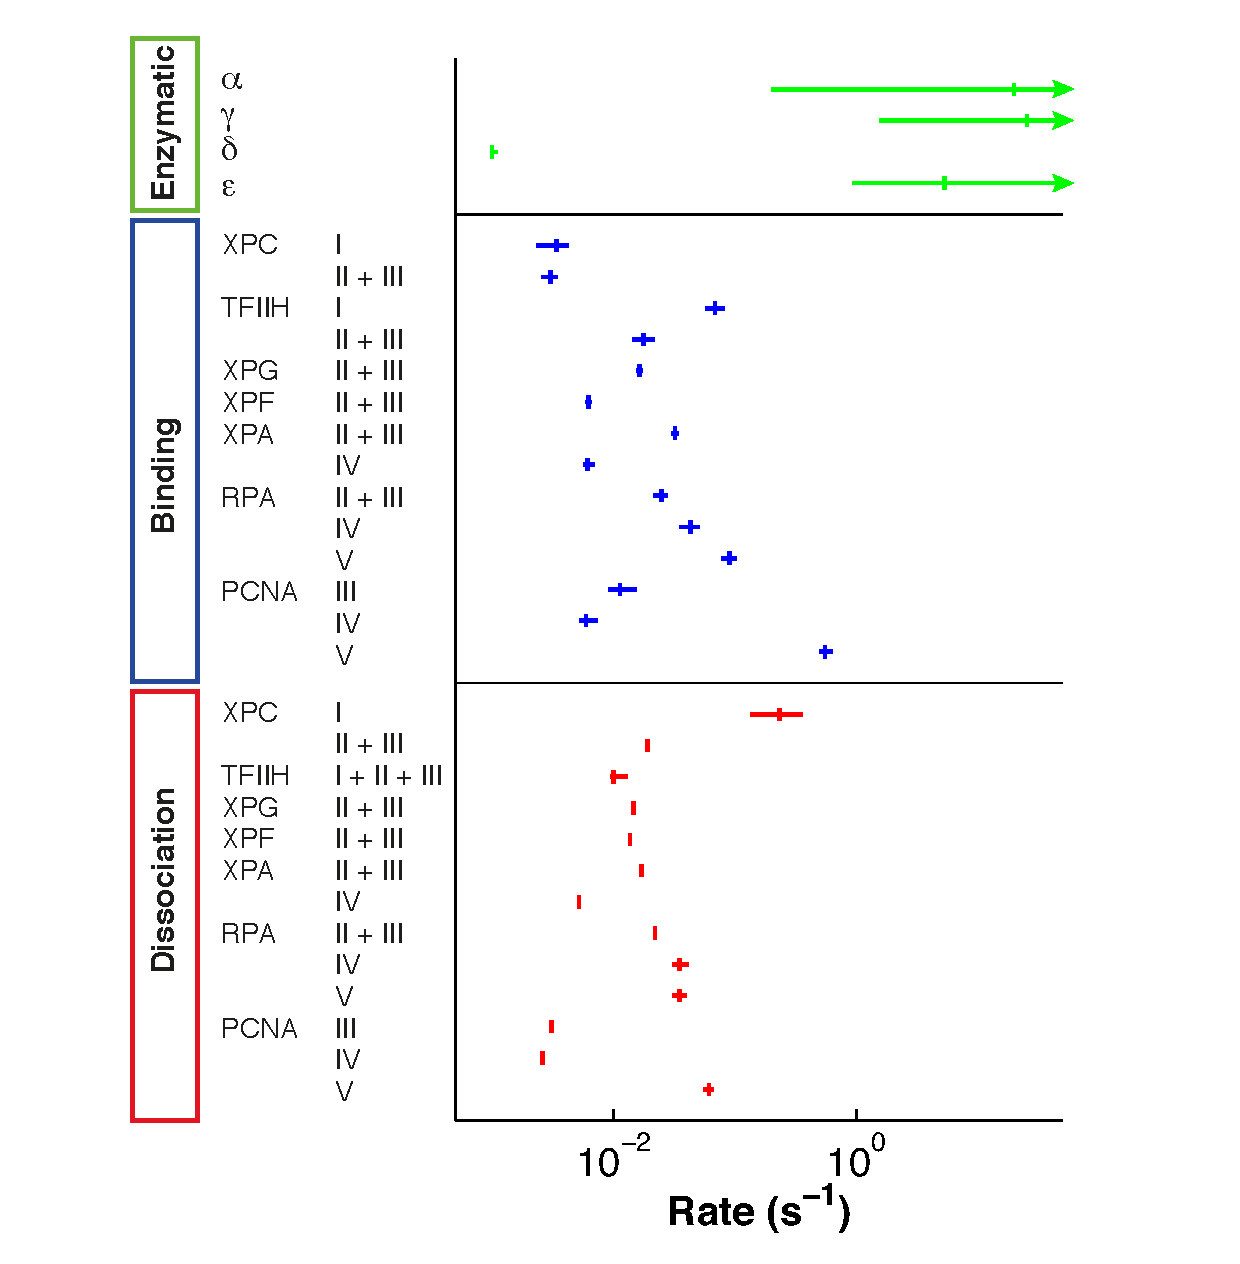
\includegraphics[width=1\textwidth]{Abbildungen/figure2_9.pdf}
		\caption{\textbf{Parametrisation identifies realistic model for NER.} Mean values (vertical bars) and confidence intervals (horizontal bars) of catalytic (green), binding (blue) and dissociation constants (red) characterizing the dynamic assembly of NER factors at the successive repair intermediates (damaged DNA I, unwound DNA II, incised DNA III, resynthesised DNA IV, rechromatinised DNA V). Arrow heads indicate infinite confidence intervals.}
		\label{fig:PLE_NER_overview}
	\end{center}
\end{figure}

Besides the slow rate of rechromatinisation $\delta$, presumably identifiable due to the slow decrease in accumulated XPA (cf.\ Figure \ref{fig:ModelFit_accu_flip}), all catalytic rates are fast. This is seen by the existence of lower bounds on the rate constants of the order of 1 $\text{s}^{-1}$. For the numerical values of the parameters see Table \ref{tab:parameter_bigTable} and Table \ref{tab:parameter_catalyticRates}. 



\begin{landscape}
	\centering
\begin{table}[t]
	
	\small{
	\begin{tabular}[angle=90]{p{2cm}ccccccc}
	\hline
	\textbf{Value}    & \textbf{ XPC} & \textbf{TFIIH} & \textbf{XPG} & \textbf{XPF} & \textbf{XPA} & \textbf{RPA} & \textbf{PCNA}  \\
	\hline
	\multicolumn{8}{l}{\textbf{Damaged DNA}} \\
	$\text{K}_{\text{d}}$({\textmu}$\text{M})$                                                  & 9.35                & 0.052 & NA &NA&NA&NA&NA     \\
	& (3.46;16.09)     &(0.044;0.072)  &&&&&   \\
	\multicolumn{8}{l}{\textbf{Unwound DNA}} \\
	$\text{K}_{\text{d}}$({\textmu}$\text{M})$                                                  & 0.864                     & 0.204                   & 0.395                 &2.446                 &0.147                    &1.222                    &NA     \\
	& (0.635;1.006)     & (0.163;0.259)             & (0.373;0.419)		&(2.344; 2.596)&(0.138;0.158)     &  (1.048;1.36)  &   \\
	\multicolumn{8}{l}{\textbf{Incised DNA}} \\
	$\text{K}_{\text{d}}$({\textmu}$\text{M})$                                                  & 0.864                     & 0.204                   & 0.395                 &2.446                 &0.147                    &1.222                    &0.388     \\
	& (0.635;1.006)     & (0.163;0.259)             & (0.373;0.419)		&(2.344; 2.596)&(0.138;0.158)     &  (1.048;1.36) 	 & (0.319;0.538)  \\
	\multicolumn{8}{l}{\textbf{Resynthesised DNA}} \\
	$\text{K}_{\text{d}}$({\textmu}$\text{M})$                                                  & NA                          &NA                         & NA                      &NA                      &0.236                   &1.167                    &0.605     \\
	&                               &                              &                           &                          &(0.222;0.27)     &  (0.924;1.521)  & (0.531;0.747)  \\
	\multicolumn{8}{l}{\textbf{Rechromatinised DNA}} \\
	$\text{K}_{\text{d}}$({\textmu}$\text{M})$                                                  & NA                          &NA                         & NA                      &NA                      &NA                         &0.538                    &0.154     \\
	&                               &                              &                           &                          &                            &  (0.438;0.645)  & (0.134;0.182)  \\
	\hline
\end{tabular}}

\begin{adjustwidth}{-1.1 cm}{}
\captionsetup{width=1.24\textwidth}
\caption{\textbf{$\text{K}_{\text{d}}$Values.} NA, not applicable. $K_d$ ($k_{\text{off}}/k_{\text{on}}$) values are given for every repair protein and arranged in columns. Reference parameter set and 95\% confidence intervals (in parentheses) are shown.}\label{tab:KdValues}
\end{adjustwidth}
\end{table}

\end{landscape}

The $K_d$ values ($k_{\text{off}}/k_{\text{on}}$), depicting the protein binding affinities to the respective DNA repair intermediate fall into a physiological realistic range between $\sim$100 nM and $\sim$1 \textmu M (cf. Table \ref{tab:KdValues}). Only XPC has a particular low affinity of 9 \textmu M, which is consistent with previous findings reporting that the time until DNA incision is mainly determined by the slow lesion recognition \cite{Luijsterburg2010}.\\        
Having an identifiable model allows us to make more precise computational predictions. For example, we can simulate the unobservable fraction of incised DNA (cf.\ Figure \ref{fig:ModelFit_intermed}, green trajectory). As the EdU incorporation measurement shows, the damaged (blue) and repaired (red) DNA kinetics are tightly coupled. This omits a higher accumulation of incised DNA.\\ 


In summary, for the development of a realistic model of the DNA repair pathway we integrated live-cell imaging data of the assembly and dissociation kinetics of all core NER factors and linked it directly to the DNA repair kinetics. The extended dataset identifies a total of 31 model parameters including 14 binding, 13 dissociation and 4 catalytic rate constants. Therefore, quantitative predictions with the model on the functioning of NER are no longer limited.  

\begin{figure}[htbp]
	\begin{center}
		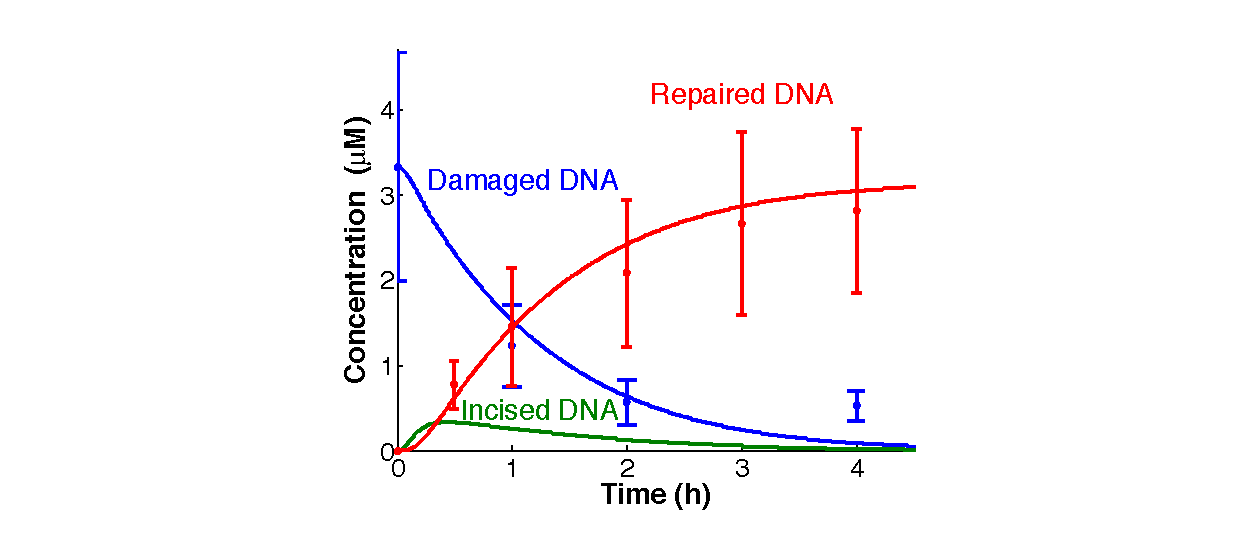
\includegraphics[width=1\textwidth]{Abbildungen/figure2_7.pdf}
		\caption{\textbf{Short delay between DNA damage removal and DNA repair synthesis omits accumulation of incised DNA.} Experimental (dots with error bars) and simulated (lines) time courses for damaged DNA (blue) and DNA repair synthesis (red). Simulated trajectories depict repair intermediate I+II for damaged DNA and repair intermediate IV+V for repaired DNA (cf.\ Figure \ref{fig:ModelStructure}). Estimated errors are depicted as shaded area. Model prediction for incised DNA (green) constitutes from DNA repair intermediate III. }
		\label{fig:ModelFit_intermed}
	\end{center}
\end{figure}




\chapter{Control analysis of the DNA repair rate}
\label{chap:robustRepair}

In chapter \ref{chap:quantData} we introduced the incorporation of EdU upon UV-irradiation as a quantitative readout for the DNA repair synthesis kinetic (\textit{cf.}\ Figure \ref{fig:EdU_measurement}). We could show that despite the pathway's complexity, DNA repair follows a mono-exponential kinetic of first order. Moreover, the repair of single lesions is distributed over a broad time with a half-time of $\sim$1.2 h. Notably, measurements on the single cell level revealed also that the half-time and hence the rate of repair is highly variable (\textit{cf.}\ Figure \ref{fig:DNArepairKinetic}B-E). So far, not only is the origin of this heterogeneity unknown, but also how the cell faces this highly variable environment.\\  
In this chapter we apply the established kinetic NER model and explore the nature of the repair rate variability. By simulating the effect of NER factor variation on the repair rate, we find that the repair-rate control is distributed among all NER factors. Exploiting the natural variability of repair proteins we can experimentally corroborate the computationally-derived finding for the NER factors XPC, TFIIH, XPA, XPF and RPA. Apart from the variability in protein expression, the model identifies the initial amount of inflicted DNA damage as major contribution determining the repair rate distribution. Both sources combined appears to be sufficient to explain the overall rate variability.\\     

The work reported in this chapter has been done in close collaboration with Paul Verbruggen who planned and conducted the experiments.

\section{Kinetic NER model predicts collective rate control}
\label{sec:repairControl}
Using PLE analysis, we identified model parameters in reasonable biological ranges (\textit{cf.}\ Section \ref{sec:identifiabilityAnalysis}), which allows us to use the model for quantitative predictions. On the basis of the simplified model result, indicating that the fast and random enzyme exchange defines the slow first-order rate kinetics (\textit{cf.}\ Section \ref{sec:toyModel}), we wanted to test whether this concept of multi-protein rate control also applies on the realistic NER model. To determine the response of a system to changes in the environment, one can calculate the response coefficients $\tilde{R}_i$ \label{sec:reponseC} \cite{Hofmeyr1991,Fell1992}. Accordingly, we can quantify the relative change in the repair rate $\nu$ as a function of the relative change in the protein concentration $C_i$ ($i$ = XPC, TFIIH, XPG, XPA, XPF, RPA, PCNA).

\begin{equation}
\tilde{R}_i = \frac{\partial \, \text{ln} \, \nu}{\partial \, \text{ln} \, C_i}.
\label{eqn:responseCoefficients}
\end{equation}

The inverse of $\nu$ is the characteristic time $\tau_R$ that represents the time duration for the repair reaction $R$. Hence, Eqn.\ \ref{eqn:responseCoefficients} can be rewritten as

\begin{equation}
\tilde{R}_i = \frac{C_i}{\tau_R^{-1}} \frac{\partial  \, \tau_R^{-1}}{\partial \,  C_i}.
\label{eqn:rC_characteristicTime}   
\end{equation}

$\tau_R$, in turn, can be directly approximated from the distribution of repaired DNA states $y^R_\pi(t)$ (\textit{cf.}\ Eqn.\ \ref{eqn:DNAstatesModel}), which include the modelled DNA intermediates for resynthesised and rechromatinised DNA. By taking the ratio between the first ($\mu^{(1)}$) and the zeroth ($\mu^{(0)}$) central moment of the distribution we derive the reaction-specific mean time 

\begin{equation}
\tau_{R} = \frac{\mu^{(1)}}{\mu^{(0)}}, 
\label{eqn:meanreactiontime}   
\end{equation}

with

\begin{equation}
\mu^{(m)} = \int_0^\infty t^m \, y^R_\pi(t)\, dt.
\label{eqn:moments}   
\end{equation}


To ensure the convergence of the integral we subtract all repair synthesis states (IV + V) from the initial amount of damages $y^{\text{I}}_{00} = $ 3.33 \textmu M at time t = 0.

\begin{equation}	
\tau_{\text{syn}}=\frac{\int_0^\infty t \, (y^I_{00}(0)-( \sum_ \pi  y_\pi^{IV}(t)+\sum_ \pi  y_\pi^{V}(t))) dt}{\int_0^\infty y^I_{00}(0)-( \sum_ \pi  y_\pi^{IV}(t)+\sum_ \pi  y_\pi^{V}(t))\; dt}
\end{equation}

Using $\tau_{\text{syn}}$ in Eqn.\ \ref{eqn:rC_characteristicTime} we derive the response coefficients for the repair synthesis rate, which are uniformly small with $\sim$0.3 and below (\textit{cf.}\ Figure \ref{fig:controlCoefficients}). This result implies that there is no single repair protein whose effect on the repair speed could be interpreted as rate-limiting. A similar result is obtained for the rate of re-synthesis response coefficients (\textit{cf.}\ Figure \ref{fig:cc_rateOfincision}), with the characteristic time

\begin{equation}
\tau_{\text{inc}}=\frac{\int^\infty_0 \,t \,\sum_{x=I}^{\text{III}} \sum_ \pi  y_\pi^x(t)\,dt}{\int^\infty_0  \,\sum_{x=I}^{\text{III}} \sum_ \pi  y_\pi^x(t)\,dt}.
\end{equation}    



\begin{figure}[htbp]
	\begin{center}
		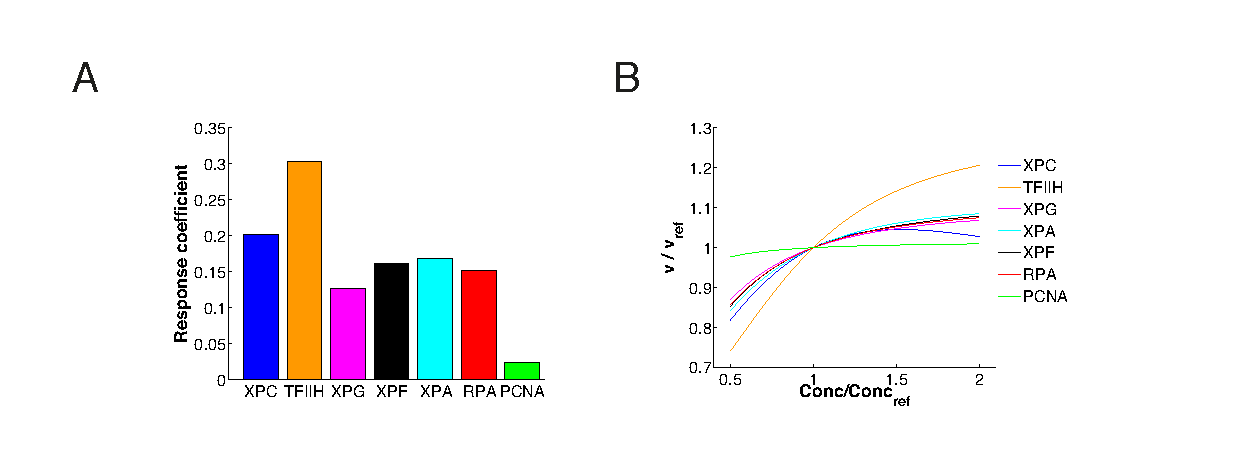
\includegraphics[width=1\textwidth]{Abbildungen/figure3_1.pdf}
		\caption{\textbf{Collective control of the repair rate.} A) Response coefficients for seven repair factors (XPC, TFIIH, XPG, XPA, XPF, RPA, PCNA) are small and uniformly distributed. B) Prediction profile likelihood indicate small prediction confidence bounds for each response coefficient. 95\% threshold is given by the $\chi^{2}$ distribution with one degree of freedom.}
		\label{fig:controlCoefficients}
	\end{center}
\end{figure}

\paragraph{Prediction profile likelihood}
To obtain realistic confidence bounds for the response coefficients we perform a prediction profile likelihood estimation \cite{Kreutz2012,Hinkley1979}. The predicted response coefficients $\tilde{R} = F(D_{\text{pred}},\theta)$ are considered as model outcomes $F$ for a predicted experimental design $D_{\text{pred}}= (z_{\text{pred}},t_{\text{pred}},u_{\text{pred}})$. $D_{\text{pred}}$ specifies a prediction observable $z_{\text{pred}}$ at time point $t_{\text{pred}}$ given the externally controlled stimulation $u_{\text{pred}}$. As defined in Eqn.\ \ref{eqn:observable} $z_{\text{pred}}(t_{\text{pred}},\theta)$ comprises a model simulation that can be mapped to experimentally observable quantities. Analogous to Eqn.\ \ref{eqn:PL}, the prediction profile likelihood 
\begin{equation}\label{sec:ppl}
PPL(\tilde{R}) = \max_{\theta^\ast \in \{\theta \lvert F(D_{\text{pred}},\theta)=\tilde{R}\}} L(z_k^\dag \lvert \theta^\ast,\tilde{r}) 
\end{equation}   

is obtained by maximization over the model parameters satisfying the constraint that the model response $F(D_\text{pred}, \theta^\ast)$ after fitting is equal to the considered value $\tilde{r}$ for the prediction $\tilde{R}$ with respect to the measured data $z_k^\dag$. This procedure is repeated for continuous variations of $\tilde{R}$. The model response can then be formulated as 

\begin{equation}
\Delta X_{\theta_l}^2(\tilde{r}) = \min_{\{\theta, \tilde{r} \in \tilde{R}  \}} \left( \chi^{2} (\theta,\tilde{r} )\right)
- \quad  \min_{\theta} \quad  \left( \chi^{2} (\theta)\right),
\end{equation}

which describes the difference between the global $\chi^{2}$ minimum and the best fit with $r$ included into the objective function. Similar to Eqn.\ \ref{eqn:confidenceIntervals} we can determine prediction confidence bounds 

\begin{equation}
PCI_{1-a}^{D_{\text{pred}},z_k^\dag} = \{\tilde{r}\textbar \Delta X_{\theta_l}^2(\tilde{r})\leq Q_{\chi^{2}}(1-a,1)\},
\label{eqn:confidenceIntervalsPPL}
\end{equation}

which include the set of predictions $\tilde{R} = F(D_{\text{pred}},\theta)$ for which -$2\log(PPL)$ is below the threshold given by the $\chi^{2}$-distribution. The PPLs were computed within the d2d-framework \cite{Raue2013} using the CVODE package \cite{Hindmarsh2005} for the numerical integration of the ODEs together with the sensitivity equations (\textit{cf.}\ Section \ref{sec:maximumLL}).
By applying the PPL analysis for each response coefficient we find that all of them are identifiable indicating how well the model predictions are determined by the data (\textit{cf.}\ Figure \ref{fig:controlCoefficients}B).\\ The moderate response predicted by the response coefficients also holds true for larger variations in the repair factor concentration (\textit{cf.}\ Figure \ref{fig:R_largeProteinVariation}). The linear approximation (on which the response coefficients are based on) yields a reasonable description for about two-fold concentration decreases or increases (corresponding to a knock-down or overexpression experiment), while for very large decreases the repair rate drops eventually to zero (corresponding essentially to a gene knock-out). From this result we can conclude that the kinetic NER model predicts a collective NER factor control of the repair rate. Consequently, the repair pathway appears robust against natural fluctuations in repair protein expression.  


\begin{figure}[htbp]
	\begin{center}
		
\includegraphics[width=1\textwidth]{Abbildungen/figure3_1_b.pdf}
		\caption{\textbf{Moderate repair rate response against natural NER factor expression variability.} Repair rate $\nu$ as a function of concentration changes in individual repair factors. Simulated repair rates are normalised by the reference rates, which are predicted by the model when applying the experimentally measured NER factor concentrations $\text{Conc}_{\text{ref}}$.} 
		\label{fig:R_largeProteinVariation}
	\end{center}
\end{figure}


\section{Exploiting natural variability in protein expression to quantify rate control}
\label{natural_Variability_m}


To corroborate the model prediction of a distributed repair rate control (\textit{cf.}\ Section \ref{sec:repairControl}), we developed an experimental set-up for the investigation of single repair factors and their quantitative influence on the repair rate. In particular, we asked whether there is a measurable response in the repair rate despite the natural occurring variability in protein expression. By capturing the integrated nuclear fluorescence intensity of antibody-stained repair proteins we derive the expression values for XPC, TFIIH, XPA, XPF and RPA. (\textit{cf.}\ Figure \ref{fig:accuImage}B).
\begin{figure}[h!]
	\begin{center}
		\includegraphics[width=1\textwidth]{Abbildungen/figure3_2.pdf}
		\caption{\textbf{Natural variability in nuclear NER factor expression is significantly larger than measurement error.} A-E) Histograms of nuclear protein concentrations of the antibody stained NER factors XPC and TFIIH (n=470), XPF and XPA (n=565), RPA (n=487). F) Scatter plot of antibody stained XPC against XPC-eGFP stably expressed in XP-C XPC-eGFP cells. The dashed error-ellipse illustrates the proportion of natural variability and measurement noise. The black line represents the linear regression with correlation coefficient r and p-value. 95\% confidence bounds of the correlation coefficients r were estimated by non-parametric bootstrap and are given in brackets (for further details \textit{cf.}\ Section \ref{apendix:correlationAnalysis}). (Experiments by P. Verbruggen)}
		\label{fig:ProteinDist}
	\end{center}
\end{figure}

\clearpage
For these five individually measured NER factors the expression variability was quantified by calculating the coefficient of variation ($CV$; standard deviation divided by the mean), which is on average $\sim$0.37 (\textit{cf.}\ Figure \ref{fig:ProteinDist}A-E). Table \ref{tab:proteinVariability} gives the means and standard deviations from at least three biologically independent measurements of the expressed protein cell-to-cell variability.




\begin{table}[t!]
	\centering
	\begin{tabular}{cccccc}
		\hline
		\rule{0pt}{2ex}
		&\textbf{XPC} & \textbf{TFIIH} & \textbf{XPA} & \textbf{XPF} & \textbf{RPA}\\ \hline
		\rule{0pt}{3ex}
		$\mathbf{CV}$: & 0.34 $\pm$ 0.05 & 0.33 $\pm$ 0.02 & 0.33 $\pm$ 0.03 & 0.4 $\pm$ 0.04 & 0.44\\ \hline
		
	\end{tabular}
	\caption{\textbf{Mean and standard deviation of the $CV$ in nuclear XPC, TFIIH, XPA and XPF expression.} Distributions for nuclear protein expression were acquired in $\text{n}_{\text{b}}^{\text{XPC}}$ = 5, $\text{n}_{\text{b}}^{\text{TFIIH}}$ = 3, $\text{n}_{\text{b}}^{\text{XPA}}$ = 3, $\text{n}_{\text{b}}^{\text{XPF}}$ = 3 and $\text{n}_{\text{b}}^{\text{RPA}}$ = 2 independent biological replicates. Within each measurement between n = 250 and n = 572 with an average of n = 477 cells were analysed.}\label{tab:proteinVariability}
\end{table}      

To distinguish whether the measured variability is due to differences in nuclear expression or rather superimposed by measurement noise, we co-analysed XPC-eGFP stably expressed in XP-C human primary fibroblasts together with immunofluorescently labelled XPC in the same cell. Both quantities are strongly positively correlated (\textit{cf.}\ Figure \ref{fig:ProteinDist}F) suggesting a large natural variability compared to much lower measurement noise. To quantitatively validate this observation, we performed a principal component analysis (PCA) \label{sec:pca} \cite{Pearson1901}. Thereby both quantities, XPC-eGFP and antibody-stained XPC intensities, are orthogonally transformed into a new coordinate system were the new transformed variables are linearly uncorrelated. These new variables are referred to as principal components. In a two-dimensional case the variances of both principal components define an error-ellipse as illustrated in Figure \ref{fig:ProteinDist}F. Calculating the $CV$ from the smaller component we determined a relative measurement error for the antibody labelling method of $\sim$11\% showing that the technique is suitable for quantification of nuclear NER factor concentrations.
      


%The same holds true for XPA \cite{Verbruggen2014}, TFIIH, XPF and RPA in narrow confidence bounds (cf.\ Appendix \textbf{tbm}).
Before exploring the direct relation between protein expression variability and the speed of repair we tested whether higher protein amounts in the nucleus correlate with the accumulation of NER factors in the locally damaged area. In correspondence to previous findings for XPG \cite{Luijsterburg2010} there is a significant positive correlation between the nuclear XPC-eGFP expression and its local accumulation at the DNA lesions (\textit{cf.}\ Figure \ref{fig:Nuc_vs_DNAsynthesis}A) sixty minutes after UV irradiation. Consequently, we conclude that the DNA lesions are not saturated, and thus, a higher NER factor concentration could potentially accelerate the repair rate.\\
\begin{figure}[h!]
	\begin{center}
		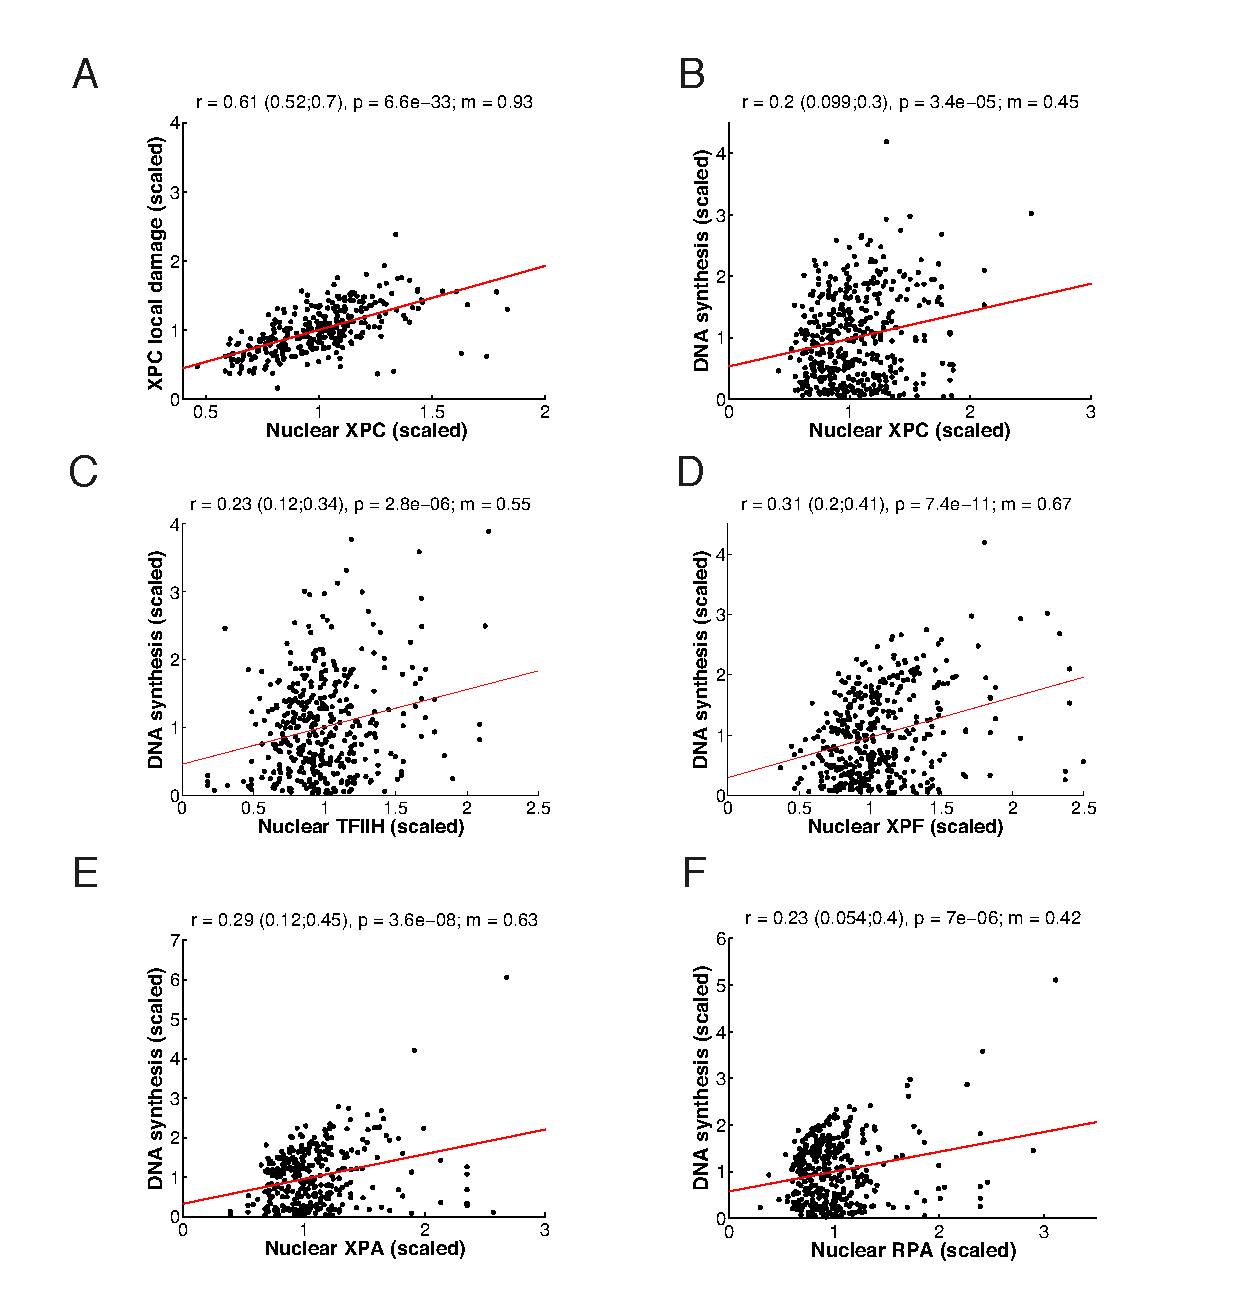
\includegraphics[width=1\textwidth]{Abbildungen/figure3_3.pdf}
		\caption{\textbf{Natural expression variability of the repair factors XPC, TFIIH, XPF, XPA and RPA has small effect on DNA repair synthesis.} A) Scatter plot of accumulated XPC in local damage against the nuclear XPC concentration (n=303) 60 minutes post irradiation. B-F) DNA synthesis correlated with the endogenous concentration of XPC (n=425), TFIIH (n=220), XPF (n=425), XPA (n=350) and RPA (n=383) 60 minutes post irradiation. A-F) Red lines represent linear regression with correlation coefficient r, p-value and slope m. 95\% confidence bounds of all correlation coefficients r were estimated by non-parametric bootstrap and are given in brackets (for further details \textit{cf.}\ Section \ref{apendix:correlationAnalysis}). (Experiments by P. Verbruggen)}
		\label{fig:Nuc_vs_DNAsynthesis}
	\end{center}
\end{figure}

\clearpage
In fact, the nuclear protein concentrations for all five antibody-stained repair factors and the amount of incorporated EdU after one hour were weak, but still significantly correlated as indicated by the correlation coefficients and the corresponding small p-values (\textit{cf.}\ Figure \ref{fig:Nuc_vs_DNAsynthesis}B-F). Remarkably, the dependency between protein concentration and EdU response, characterized by the slope of the regression line is very evenly distributed (\textit{cf.}\ Figure \ref{fig:controlCoefficients}A). This agrees with the \textit{in silico} finding that the kinetic control of the measured repair factors is uniformly distributed and that the rate of repair synthesis is robust against natural variations in the repair protein expression.\\ 
To reinforce the conclusion of a robustness DNA repair rate we compared the repair factor expression and its consequence on the repair variability in different cell lines. In contrast to indirectly labelled XPC in Hela cells \cite{Verbruggen2014} or in human primary fibroblasts (\textit{cf.}\ Figure \ref{fig:ProteinDist}), the expression of stably transfected XPC-eGFP into XP-C patient cells is much broader distributed. Its $CV$ has a value of $\sim$1, which is up to four times larger compared to XPC variability in Hela or fibroblasts cells (compare Figure \ref{fig:consistVariability}A with Figure \ref{fig:ProteinDist}A and \cite{Verbruggen2014}). \\
In Hela cells and XPC-eGFP complemented XP-C cells we measured EdU incorporation after 1, 2 and 3 hours post UV-irradiation (\textit{cf.}\ Figure \ref{fig:consistVariability}). At all three time points the distributions of newly-incorporated DNA were nearly congruent suggesting that DNA repair follows the same kinetics regardless of the cell type and the corresponding NER factor expression variability. This result allows to generalize the concept of a robust repair rate for different cell types and their cellular environments.\\ 






\section{Variable NER factor expression and inflicted lesions account for the distribution of repair rates} 
\label{sec:variabilityAnalysis}

Comparing the measured EdU incorporation as a function of NER factor concentration and the predicted response coefficients quantitatively (\textit{cf.}\ Section \ref{natural_Variability_m}), we noted that the measured repair responses towards changes in the nuclear protein concentration are consistently two to four-fold larger than the mathematically calculated values (compare the slopes m in \ Figure \ref{fig:Nuc_vs_DNAsynthesis}B-F with the response coefficients $\tilde{R}_i$ in Figure \ref{fig:controlCoefficients}A). This result suggests that the measured repair-rate response is not solely explained by the model-predicted response coefficients. It remains to be clarified, whether this discrepancy is due to a so far unknown additional NER component intrinsically contributing to the pathway control, or whether there is an external mechanism coordinating the NER factor expression and thereby superimposing the mathematically predicted response coefficients.

\begin{figure}[htbp]
	\begin{center}
		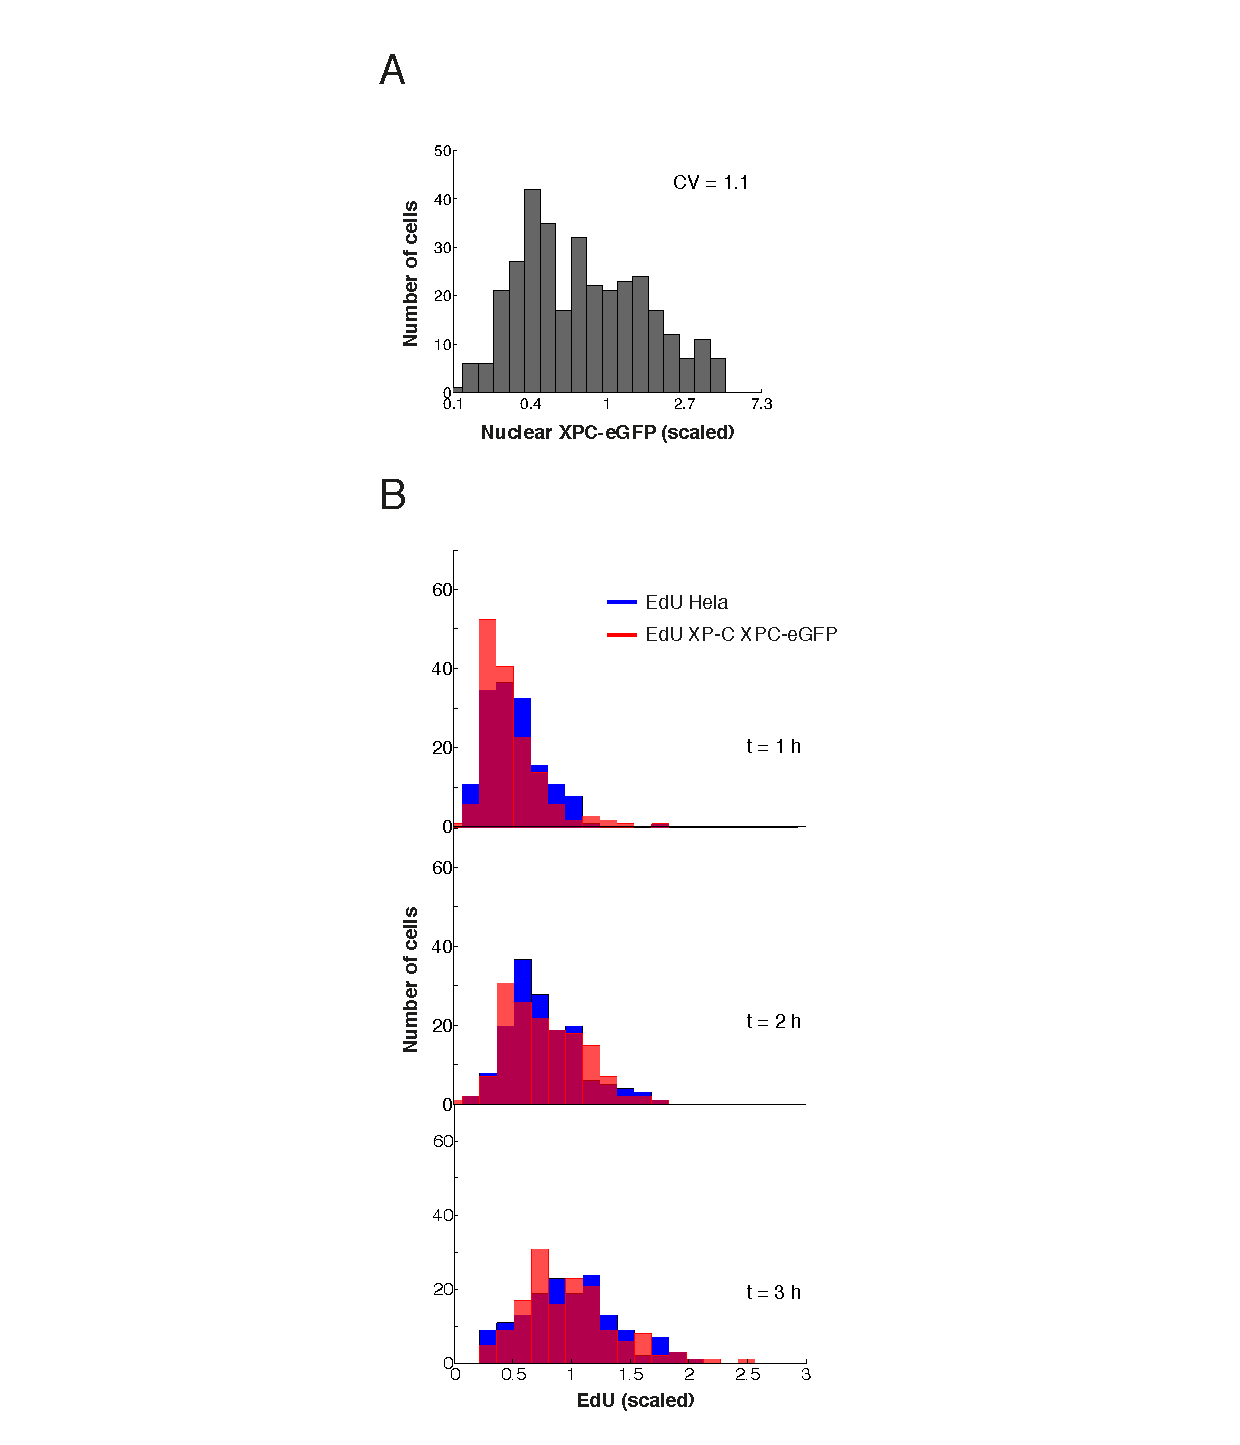
\includegraphics[width=1\textwidth]{Abbildungen/figure3_4.pdf}
		\caption{\textbf{Variability of repair synthesis is comparable between XPC-eGFP complemented XP-C patient cell lines and native NER.} A) Distribution of nuclear XPC-eGFP concentrations stably expressed in XP-C cells (n=332). B) Comparison of incorporated EdU in local damages in Hela cells (blue) and XPC-eGFP complemented XP-C cells (red) after 1, 2 and 3 hours post UV-irradiation (n=154 cells per time point per cell line). (Experiments by P. Verbruggen)}
		\label{fig:consistVariability}
	\end{center}
\end{figure}

While searching for additional factors affecting the repair rate response we noticed the broad scatter of incorporated EdU, which appears to increase for larger protein concentrations (\textit{cf.}\ Figure \ref{fig:Nuc_vs_DNAsynthesis}B-F). This variability indicates that, in addition to the repair proteins, there might be further sources of cell-to-cell heterogeneity, which could be also involved in the regulation of the repair rate. To this end, we measured the amount of UV-inflicted DNA lesions by indirect (immuno)cytochemistry to determine how the distribution of pore sizes would propagate (\textit{cf.}\ Figure \ref{fig:accuMethod}B). The distribution of DNA damage captured immediately after UV-irradiation very much resembles the variable EdU incorporation after 4 hours (\textit{cf.}\ Figure \ref{fig:DamageDist}), which is also confirmed by the similar $CV$s. These data suggest that the amount of DNA lesions contributes to the cell-to cell variability in the repair-rate.  


\begin{figure}[t!]
	\begin{center}
		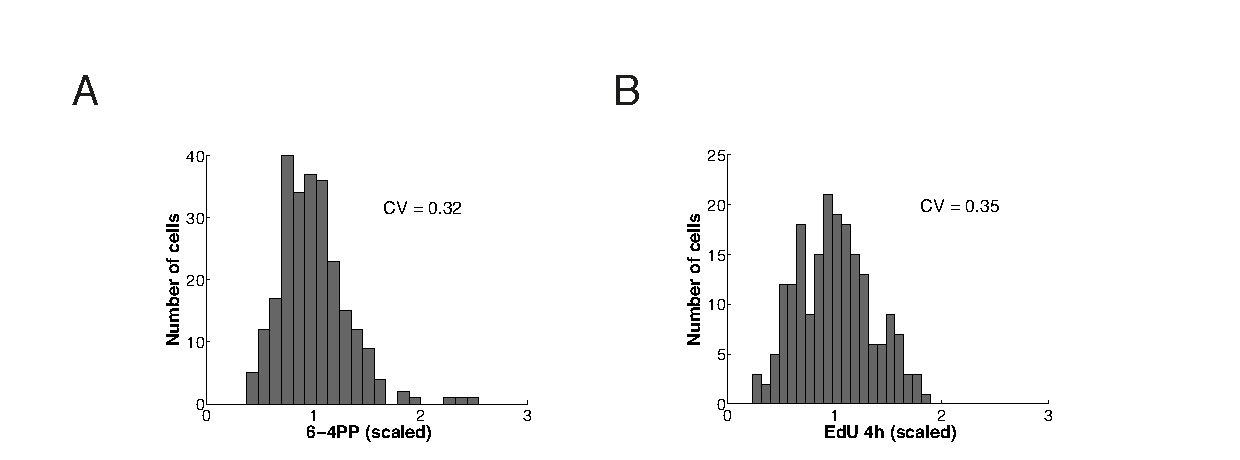
\includegraphics[width=1\textwidth]{Abbildungen/figure3_5.pdf}
		\caption{\textbf{Distributed amount of inflicted DNA damages contributes to repair rate variability.} A) XP-C XPC-eGFP cells were locally UV-irradiated with an intensity of 100 J/$\text{m}^\text{2}$. DNA damages were quantified by indirect immunofluorescence microscopy in n=250 cells from five experiments. B) XP-C XPC-eGFP cells were locally irradiated and cultivated for 4 hours in the presence of EdU before fixation. Fluorescence signals were measured in n=198 cells derived from three independent experiments. (Experiments by P. Verbruggen)}
		\label{fig:DamageDist}
	\end{center}
\end{figure}

\begin{figure}[htbp]
	\begin{center}
		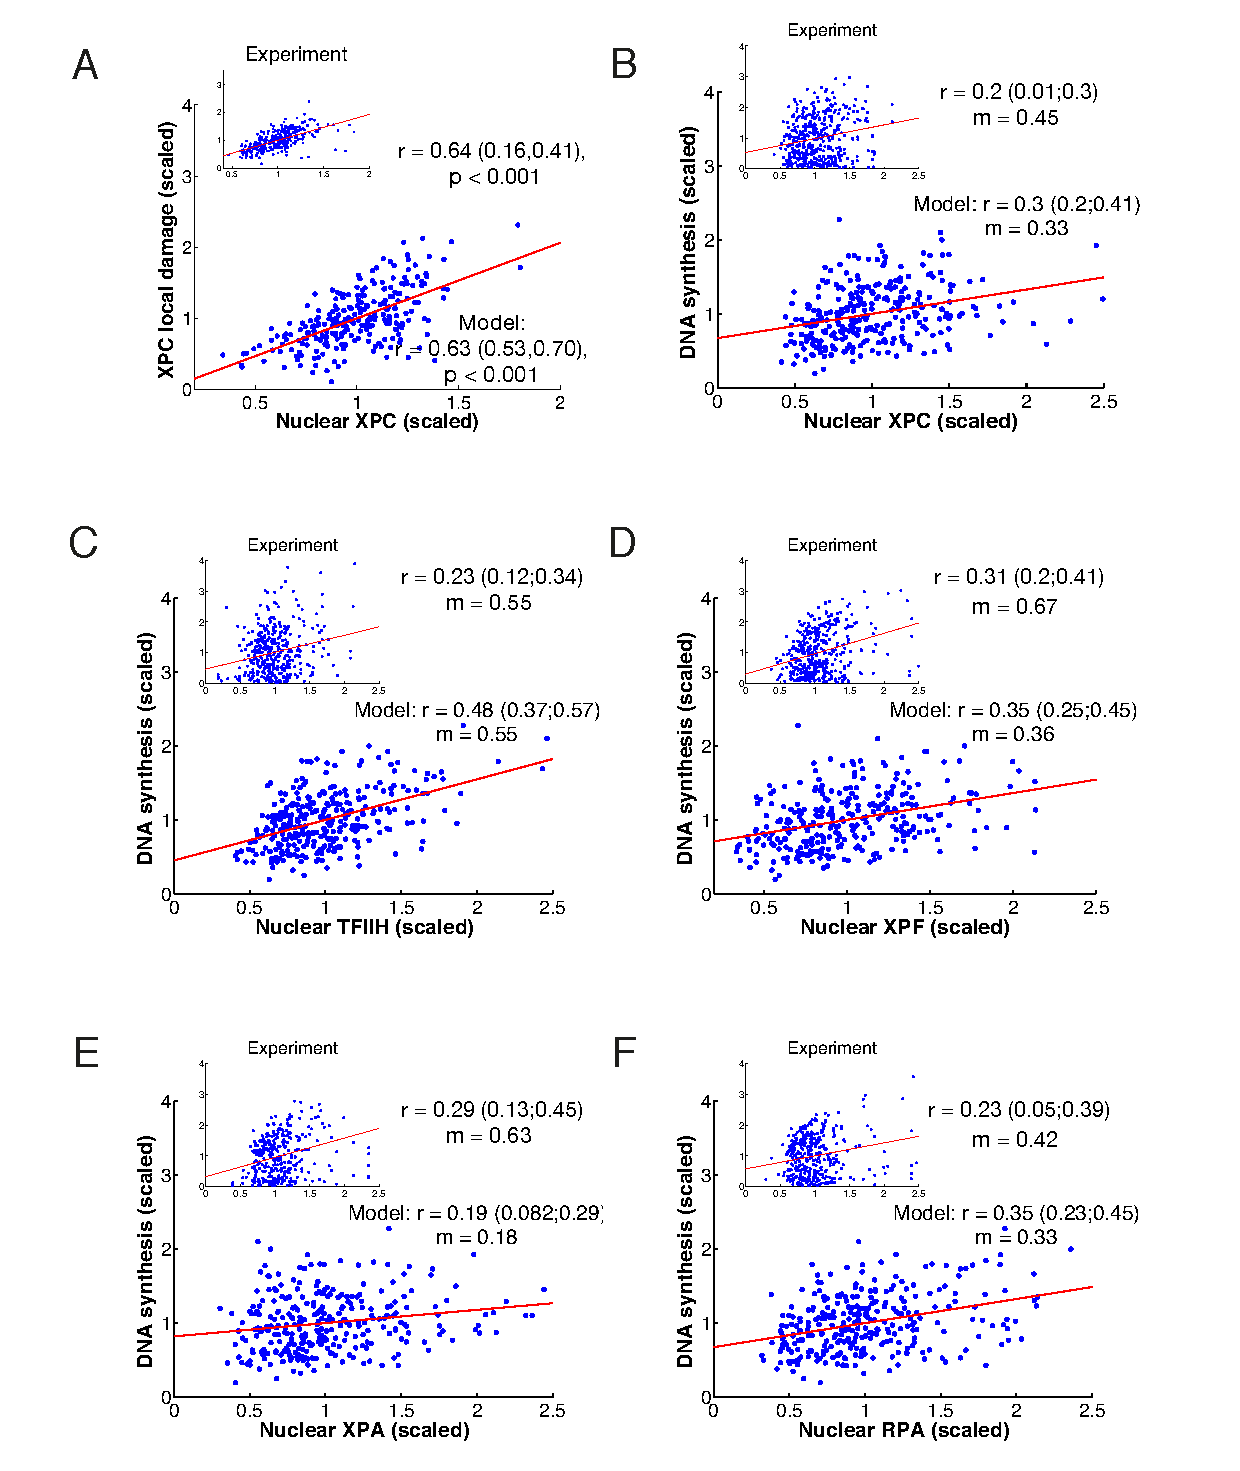
\includegraphics[width=1\textwidth]{Abbildungen/figure3_6.pdf}
		\caption{\textbf{Quantitative comparison between measured and simulated repair resynthesis in response to variable NER factor concentrations.} A) Simulated scatter plot of locally accumulated XPC against the nuclear XPC concentration. For comparison the experimentally measured scatter plot is given in reduced size.  B-F) Comparison between measured (scatter plot in reduced size) and simulated correlation of DNA synthesis and nuclear XPC concentration. A-F) Red lines represent linear regression with correlation coefficient r, p-value (only in A) and slope m. 95\% confidence bounds of all correlation coefficients r were estimated by non-parametric bootstrap and are given in brackets (for further details \textit{cf.}\ Section \ref{apendix:correlationAnalysis}). Nuclear protein expression values are scaled by dividing by the mean value. (Experiments by P. Verbruggen)}
		\label{fig:Model_dataComp}
	\end{center}
\end{figure}

To find out whether the heterogeneity in nuclear NER factor expression, together with the distributed amount of initial DNA damages, would be sufficient to explain the variability in the repair rate we tried to reproduce the EdU response measurements with the evolved quantitative model introduced in Chapter \ref{chap:kineticNERmodel}. Thus, we simulated the model several hundred times in correspondence with the number of measured cells. For each simulated cell nuclear NER factor concentrations and the amount of local damages were randomly drawn from log-normal distributions in accordance with the experimentally determined $CV$s (\textit{cf.}\ Figure \ref{fig:ProteinDist} and Figure \ref{fig:DamageDist}) and the previously measured mean values \cite{Luijsterburg2010}. For PCNA and XPG we took the averaged $CV\sim$0.33 derived from the measured distributions. \\
For XPC the simulated scatter plot for the accumulation of the nuclear repair factor at sites of local damage agrees remarkably well with the measured data (\textit{cf.}\ Figure \ref{fig:Model_dataComp}A, compare enlarged, simulated correlation with the smaller inlay, of the experimentally observed scatter plot). Qualitatively, the same holds true for the comparison between simulated and measured EdU incorporation as a readout for DNA resynthesis in response to changes in the concentration of the repair factors (\textit{cf.}\ Figure \ref{fig:Model_dataComp}B-F). It should be noted that the simulated slopes representing the overall repair rate response are slightly elevated compared to the calculated response coefficients (\textit{cf.}\ Figure \ref{fig:controlCoefficients}), clearly marking the influence of the introduced distribution of DNA damages. In particular for XPA, XPF and RPA though, the simulated slopes are still significantly smaller than the measurement-based regression estimates (\textit{cf.}\ Table \ref{tab:responsecomparison}). 
\begin{table}[t!]
	\centering
	\begin{tabular}{lccc}
		\hline
		\rule{0pt}{2ex}
		\hspace{-0.1cm}\textbf{Repair protein} & \textbf{Measured $\boldsymbol{ \mathit{m} }$} & \textbf{Simulated $\boldsymbol{ \mathit{m} }$} & $\mathbf{\tilde{R_i}}$  \\
								&	(\textit{cf.}\ Figure \ref{fig:Nuc_vs_DNAsynthesis})&	(\textit{cf.}\ Figure \ref{fig:Model_dataComp})& (\textit{cf.}\ Figure \ref{fig:controlCoefficients})\\	 \hline					
		\rule{0pt}{3ex}
		\hspace{-0.1cm}\textbf{XPC}: & 0.36 $\pm$ 0.21 & 0.33 & 0.20 \\ 
		\textbf{TFIIH}: & 0.45 $\pm$ 0.08 & 0.55 & 0.30 \\ 
		\textbf{XPA}: & 0.75 $\pm$ 0.17 & 0.18 & 0.16 \\ 
		\textbf{XPF}: & 0.62 $\pm$ 0.10 & 0.36 & 0.15 \\ 
		\textbf{RPA}: & 0.37  & 0.33 & 0.15 \\ 
		\hline
		
		
	\end{tabular}
	\caption{\textbf{Comparison of the measured and predicted repair responses caused by fluctuations of the NER factor concentrations.} Changes in DNA repair synthesis in response to variations of the nuclear NER factor abundance quantified i) from experimental data 
	 (mean $\pm$ SD of the regression slopes $m$ from $\text{n}_{\text{XPC}}$ = 5, $\text{n}_{\text{TFIIH}}$ = 3, $\text{n}_{\text{XPA}}$ = 3, $\text{n}_{\text{XPF}}$ = 3 and $\text{n}_{\text{RPA}}$ = 2 independent biological replicates; within each measurement between n = 250 and n = 572 with an average of n = 477 cells were analysed), ii) from model simulation (nuclear NER factor concentrations and the amount of local damages were randomly drawn from log-normal distributions in accordance with the experimentally determined $CV$s (\textit{cf.}\ Figure \ref{fig:ProteinDist} and Figure \ref{fig:DamageDist})) and predicted iii) by the response coefficients $\tilde{R_i}$ (\textit{cf.}\ Section \ref{sec:repairControl}). }\label{tab:responsecomparison}
\end{table}
This indicates that we still miss out on an essential, perhaps intrinsic, factor regulating the repair-rate response. \\    
To locate the lacking control, we first asked whether the natural variability, contributed by the NER factor expression variability and the distribution of inflicted lesions, can explain the distribution of the repair rate. Assuming that the repair rate $\nu$ is linearly dependent on the initial amount of inflicted lesions $L$ and, as estimated in Section \ref{firstOrderRateKinetic}, also on the nuclear repair-factor concentrations $C_i$ ($i=1,\ldots,N$), we can apply the general law of error propagation
%and hence 'sums up' according to the response coefficients predicted by the model

\begin{equation}
\sigma(\nu) = \sqrt{\sum_{i = 1}^{N} \left(\frac{\partial \nu}{\partial C_i}\sigma(C_i) \right)^2 + \left(\frac{\partial \nu}{\partial L}\sigma(L)\right)^2 }.
\label{eqn:lawoferrorPropagation}
\end{equation} 
Introducing the predicted response coefficients $\tilde{R_i}$ we can estimate the overall repair rate variability $CV_{\nu}$ with
\begin{equation}
CV_{\nu} = \sqrt{CV_{L}^2 + \sum_{i = 1}^{N}(\tilde{R_i} \, CV_i)^2},
\label{eqn:lawOfErrorPropI}
\end{equation}
where $CV_{i}$ and $CV_L$ denote the coefficients of variation of the distributions of the individual repair factors and initial amount of lesions. Obviously, the response coefficient for the initial amount of inflicted lesions is 1. Including the variability for the initial amount of inflicted lesions $CV_L\sim$0.32 (\textit{cf.}\ Figure \ref{fig:DamageDist}A) and the average $CV_i \sim$0.33 for each repair factor, we can determine the repair rate variability with $CV_{\nu} \sim$0.35. This is around 20\% less than the measured $CV_{\nu} \sim$0.45 after one hour post UV-irradiation (\textit{cf.}\ Figure \ref{fig:CV_Var_comp}).\\
To dissect the contribution of the individual factors to the
overall variability, we computed the effect of heterogeneity in only one factor on repair synthesis. Accordingly, for each $CV$-trajectory in Figure \ref{fig:CV_Var_comp} we determined the $CV_{\nu}$ by simulating the repair rate for 500 cells and drawing only one factor randomly. The largest contribution can be allocated to the initial amount of damages (\textit{cf.}\ Figure \ref{fig:CV_Var_comp} brown trajectory), which was responsible for about two thirds of the whole observed repair variability (\textit{cf.}\ Figure \ref{fig:CV_Var_comp} blue trajectory). Drawing all NER factors together with the initial amount of damages from their pre-determined distributions shrinks the gap between measured and simulated DNA repair variability (\textit{cf.}\ Figure \ref{fig:CV_Var_comp} blue (data) and red (simulation) trajectory). This result becomes more explicit, as seen, by comparing the strikingly matching temporal evolution of the measured and predicted distributions of repair synthesis (\textit{cf.}\ Figure \ref{fig:ModelData_tempVar}).\\
\begin{figure}[h]
	\begin{center}
		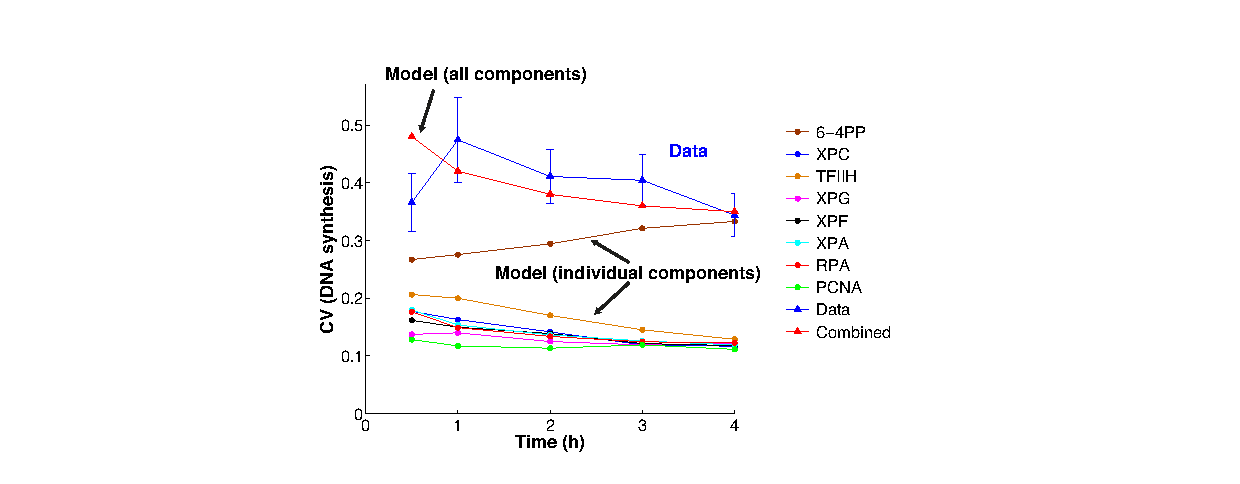
\includegraphics[width=1\textwidth]{Abbildungen/figure3_8.pdf}
		\caption{\textbf{Variability in repair synthesis results from the aggregate of initial damage variability and concentration fluctuations of each NER factor.} Each time course represents the variability in repair synthesis produced by a single component (dots) or by all components together (triangles) at a given time. For comparison the experimental measured distribution of incorporated EdU is shown in blue. Error bars depict the 95\% confidence intervals determined with non-parametric bootstrap.}
		\label{fig:CV_Var_comp}
	\end{center}
\end{figure}

\begin{figure}[h]
	\begin{center}
		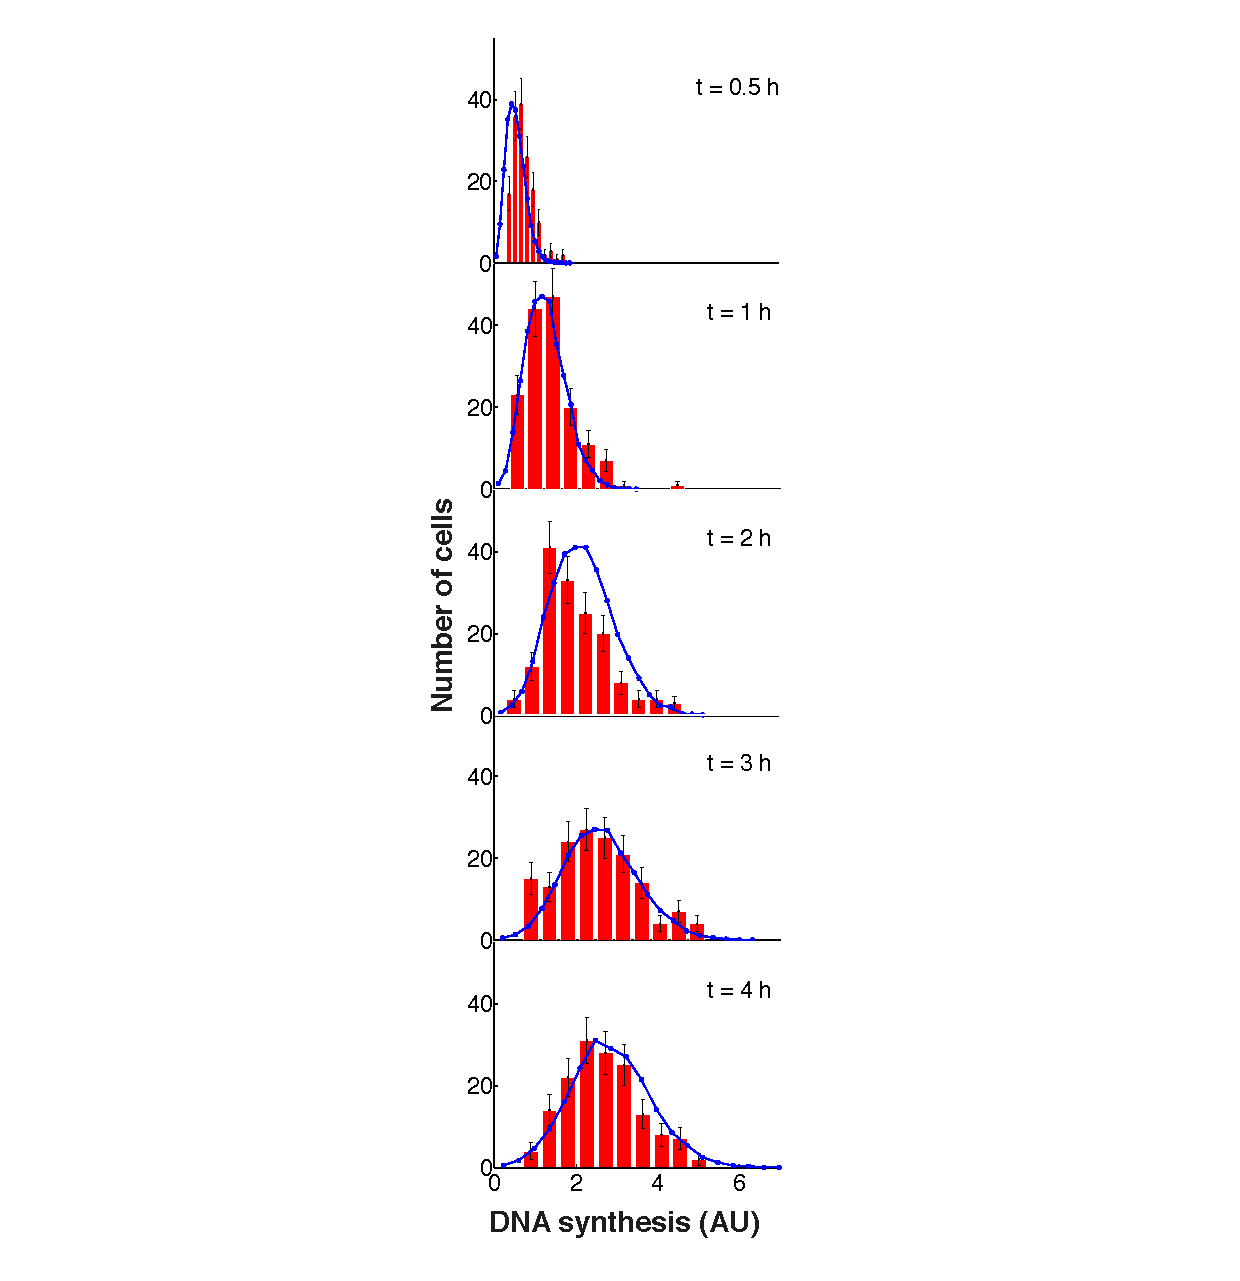
\includegraphics[width=1\textwidth]{Abbildungen/figure3_7.pdf}
		\caption{\textbf{Simulated repair rate distribution fits experimentally derived EdU incorporation.} Temporal evolution of the repair rate variation  measured in single cells after initial UV-irradiation (red histograms) and predicted from model simulations (blues lines). (Experiments by P. Verbruggen)}
		\label{fig:ModelData_tempVar}
	\end{center}
\end{figure}
\clearpage

To summarize, in this chapter we uncovered two sources of natural variability that are propagated throughout the repair process and consequently contributing to the emergent cell-to-cell variability of repair synthesis: (i) the initial amount of inflicted DNA lesions and (ii) the variation of the nuclear NER factor concentrations. 
However, the significant differences between measured and predicted repair rate responses (\textit{cf.}\ Table \ref{tab:responsecomparison}) leave space for interpretation, whether there are additional factors involved in repair, but have not been explicitly accounted for, in the model.



%\clearpage{\pagestyle{empty}\cleardoublepage}


% ************************* PART IV *****************************


\chapter{Co-expression of NER repair factors}
\label{chap:crossCorell}
The aforementioned model-aided analysis of the DNA repair process revealed a link between the emergent phenomenon of rapidly exchanging and transiently interacting NER components with the experimentally observed slow first-order kinetics of repair (cf.\ Chapter \ref{chap:quantData}). An important functional consequence of this kinetic design is that the control of the repair rate is shared by all repair factors. This manifests in the mathematical prediction of small, uniformly distributed response coefficients, which quantify the relative change of the repair rate in answer to changes in the nuclear repair protein concentration (cf.\ Section \ref{sec:repairControl}). Exploiting the natural variability in NER factor expression we experimentally corroborated the moderate control of the repair components on the repair rate. We found that compared to the model-predicted response coefficients the measured EdU response was significantly elevated (cf.\ Figure \ref{fig:Model_dataComp}). \\ 
In this chapter we will show that this discrepancy can be explained assuming that the measured response is a superposition of firstly, the response due to concentrational changes for one repair factor and secondly, an additional cross-correlation among the repair factors. To test this assumption, we experimentally investigate the potential co-expression of five repair factors (XPC, TFIIH, XPA, XPF and RPA). Surprisingly, we find that the nuclear expression of these pairwise measured repair factors is indeed strongly positively correlated, whereas there is no correlation with the repair-independent cell cycle marker Ki67 \cite{Scholzen2000}. This result suggests an additional control mechanism orchestrating NER factor expression on the pre-transcriptional level.\\ 

The microscopy experiments reported in this chapter have been planned and conducted by Paul Verbruggen (University of Amsterdam). Image segmentation was performed by Simon Eck (Division of Theoretical Bioinformatics, DKFZ). The flow cytometry analysis was done in close collaboration with Martin Teichert, who is part of the division of Vascular Oncology and Metastasis led by Prof.\ Helmut Augustin. 
 



\section{Cross-correlation affects repair response}
\label{sec:crossCorelResponse}
The finding that the measured response in DNA synthesis is about twofold higher than the model-predicted response coefficients (cf.\ Figure \ref{fig:controlCoefficients} and Figure \ref{fig:Nuc_vs_DNAsynthesis}) indicates that there is an additional factor regulating the repair response. An explanation not yet considered explanation is the potential interdependence of the NER factor expression, introduced by an external gene-regulatory mechanism. This would result in a measurable cross-correlation of the nuclear NER factor expression. Mathematically, such a factor would extend the relation between measured EdU response (cf.\ Figure \ref{fig:Nuc_vs_DNAsynthesis}) and the model-predicted response coefficients to 

\begin{equation}
\frac{C_i}{\nu}\frac{d \nu}{d C_i} = \frac{C_i}{\nu}\frac{\partial \nu}{\partial C_i} + \sum_{j \neq i} \left( \frac{C_j}{\nu}\frac{\partial \nu}{\partial C_i}\right) \left(\frac{C_i}{C_j}\frac{\partial C_j}{\partial C_i}\right), 
\label{eqn:extendedResponse}
\end{equation}    
where $\nu$ represents the rate of EdU incorporation and $C_i$ the nuclear concentration of the $i^{\text{th}}$ repair factor. From Eqn. \ref{eqn:extendedResponse} we directly measured the EdU incorporation for varying NER factor concentrations after one hour (cf.\ Figure \ref{fig:Nuc_vs_DNAsynthesis})

\begin{equation}
A_i = \frac{C_i}{\nu}\frac{d \nu}{d C_i}. \nonumber
\end{equation}

By also measuring the pairwise cross-correlations

\begin{equation}
B_{ij} = \frac{C_i}{C_j}\frac{\partial C_j}{\partial C_i} \nonumber
\end{equation}

we can derive the following system of equations


\begin{equation}
R_i + \sum_{j\neq i} B_{ij}R_j = A_i,
\label{eqn:linearEqnSystem}
\end{equation}

for $i \in$ 1,...,N and

\begin{equation}
R_i = \frac{C_i}{\nu}\frac{\partial \nu}{\partial C_i}.
\label{eqn:responseCoefficientsII}
\end{equation}

Assuming that all $B_{ii}$ = 1 Eqn. \ref{eqn:linearEqnSystem} translates into the matrix notation 
\begin{equation}
\vec{A} = B\vec{R}.
\label{eqn:matrixNotation}
\end{equation}

By inverting $B$ we can solve Eqn. \ref{eqn:matrixNotation} for the desired response coefficients directly. 


\section{Microscopy analysis of co-staining experiments}

In order to measure the cross-correlation matrix $B$ we made use of the fluorescence microscopy approach, which proved to result in accurate measurements of the nuclear repair factor expression and their UV-induced repair dynamics (cf.\ Figure \ref{fig:Nuc_vs_DNAsynthesis}). For a flexible combinatorial tagging of multiple antigens simultaneously, we used an indirect antibody-labelling protocol and established five single cell double stainings (cf.\ Table \ref{tab:co-staining} using the primary and secondary antibodies listed in Table \textbf{tbm}. 


\begin{table}[h!]
	\centering
	\begin{tabular}{cccccc}
		\hline
			\rule{0pt}{2ex}
			&\textbf{XPC} & \textbf{TFIIH} & \textbf{XPA} & \textbf{XPF} & \textbf{RPA}\\ \hline
			\rule{0pt}{3ex}
\textbf{XPC}&        X    &           X    & X            &         X    & X            \\ \hline
			\rule{0pt}{3ex}
\textbf{TFIIH}&           & -              & -            & X            & -             \\ \hline
			\rule{0pt}{3ex}
\textbf{XPA}&             &                & -            & X            & X             \\ \hline
			\rule{0pt}{3ex}
\textbf{XPF}&             &                &              & -            & -              \\ \hline
			\rule{0pt}{3ex}
\textbf{RPA}&             &                &              &              & -               \\ \hline
			\rule{0pt}{3ex}
		
	\end{tabular}
	\caption{\textbf{Immuno-fluorescence microscopy of NER factor co-expression} Crosses indicate pairwise measurement of indirectly antibody-labeled NER factor expression. Underlined crosses denote costainings involving directly labeled XPC. }\label{tab:co-staining}
\end{table}   


Two additional cross-correlation measurements were possible by directly labelling XPC with a monoclonal mouse antibody and thereby avoiding potential cross-reactions between antibodies originating from the same host species \cite{Burry2011,Giepmans2006}. The cross-correlation analysis was performed in human diploid female fibroblasts which were grown to confluency on coverslips. Analogous to the description in Section \ref{sec:local_irradiation} cells were UV-irradiated locally with a dose of 100 J/$\text{m}^\text{2}$. Cells were pre-incubated with serum-free medium containing 10 \textmu M EdU and allowed to repair for 60 minutes in an incubator. After the subsequent direct or indirect antibody labelling of two selected repair factors, cells were also incubated with a DAPI solution, which visualizes the cell's chromatin and thereby gives rise to the contour of the nucleus. For each double staining, microscopic 3-dimensional imaging was conducted on a Leica TCS SP5 II confocal microscope. All images were analysed following the protocol presented in Section \ref{subsec:AccuFlipExp}. Segmentation of the nucleus was performed on the DAPI signal, due to the large signal-to-noise ratio in this channel (cf.\ Figure \ref{fig:coStaining}A). The segmented region was then projected to the other channels and used to quantify the signal emitted by the secondary antibodies at 488 and 647 nm (cf.\ Figure \ref{fig:coStaining}B and C). For the same reason segmentation of the locally UV-irradiated chromatin region was done with the area determined from the EdU signal and then projected onto the signal of accumulated protein (cf.\ Figure \ref{fig:coStaining}D).   

\begin{figure}[t!]
	\begin{center}
		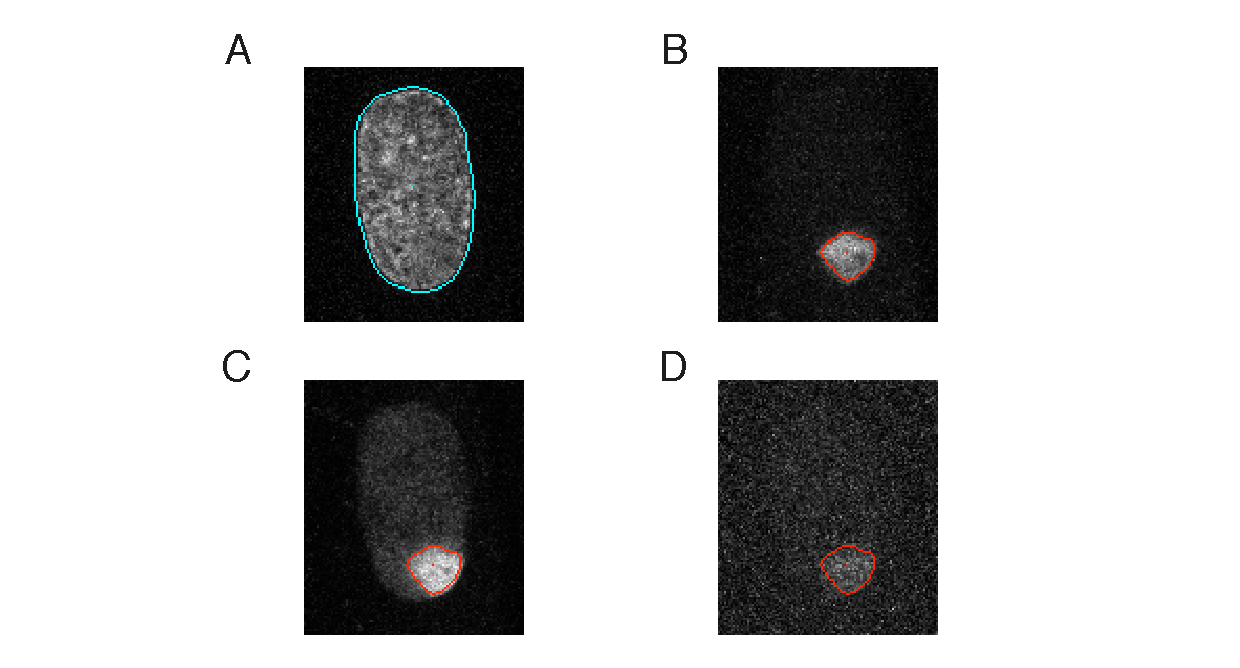
\includegraphics[width=1\textwidth]{Abbildungen/figure4_1.pdf}
		\caption{\textbf{3D fluorescence microscopy imaging of NER factor co-expression} A) DAPI-stained DNA content measured in human primary fibroblast (Life technologies). DAPI segmentation at 461 nm  (green contour line) determines nuclear dimensions. B-C) Nuclear expression of indirectly immuno-stained repair factors at 488 nm (B) and at 647 nm (C). Signals are quantified according to the nuclear contour (cyan contour line) segmented from the DAPI signal. D) DNA locally damaged by UV-irradiation and subsequently incubated for 60 minutes in the presence of 10 \textmu M EdU. Segmentation of the EdU signal is indicated by the red contour line.   }
		\label{fig:coStaining}
	\end{center}
\end{figure}

To test whether the antibody co-staining experiment is suitable for the cross-correlation analysis, we measured XPC expression with a directly labelled antibody together with an indirect immuno-staining and correlated both signals. Fitting an error ellipse to these data (cf.\ Figure \ref{fig:coExpressionData}A), as described in section  \ref{subsec:AccuFlipExp}, we estimated a relative measurement error of antibody labelling of 13\%, showing that the technique is sufficiently accurate to exploit the natural variability in protein expression for the cross-correlation analysis.
\begin{figure}[htbp]
	\begin{center}
		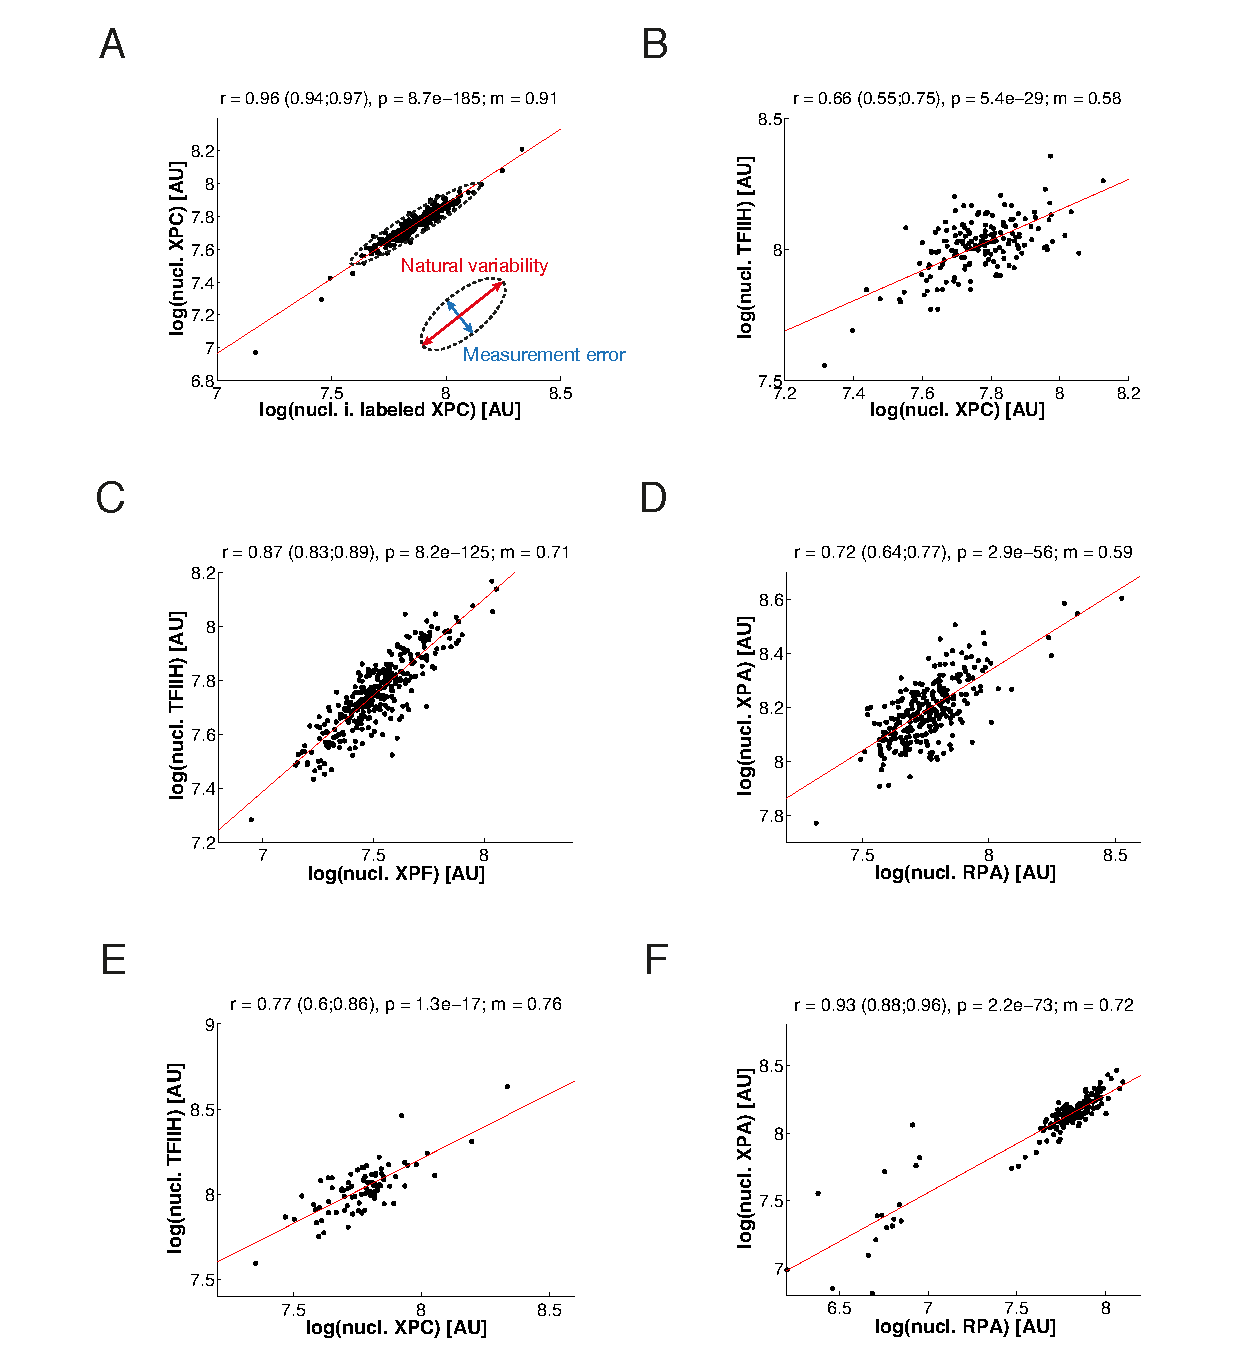
\includegraphics[width=1\textwidth]{Abbildungen/figureTAC_2.pdf}
		\caption{\textbf{NER factor cross-correlation is repair independent.} A) Scatter plot of indirectly antibody-stained XPC against a directly labelled antibody recognising XPC (n=336) as determined by quantitative (immuno) fluorescence microscopy. B-D) Pairwise correlations of indirectly antibody-labelled XPB against XPC (n=220, B), XPB against XPF (n=410, C) and XPA against RPA (n=350, D) in locally damaged cells. Expression values represent fluorescence intensities originating from the nucleus including the damaged region (signal quantification was performed analogous to \cite{Luijsterburg2010}). E-F) Scatter plots of the nuclear expression of XPB vs. XPC (n=85) and XPA vs. RPA (n=170) in undamaged cells. A-F) Red lines represent linear regression with correlation coefficient r, p-value and slope m. 95\% confidence bounds of all correlation coefficients r were estimated by non-parametric bootstrap and are given in brackets. }
		\label{fig:coExpressionData}
	\end{center}
\end{figure}

\noindent As it turns out, all pairwise correlations of the measured co-staining experiments (cf.\ Table \ref{tab:co-staining}) are strong positively correlated with correlation coefficients between 0.66 and 0.88 (cf.\ Figure \ref{fig:coExpressionData}B-D and Figure \ref{fig:nuklearCrosscorrelation}). Notably, the result is irrespective of whether the acquired fluorescence signal is taken from the whole nucleus including the locally damaged area or only from the undamaged chromatin region (cf.\ Figure \ref{fig:coExpressionData}B-D and \ref{fig:coExpressionData}E-F). This suggests that the correlation of nuclear NER factors is independent of the ongoing repair. As a consequence, we suspect that the regulatory mechanism determining the protein concentrations lies on a preceding level such as transcription or translation.\\  


%\begin{figure}[htbp]
%	\begin{center}
%		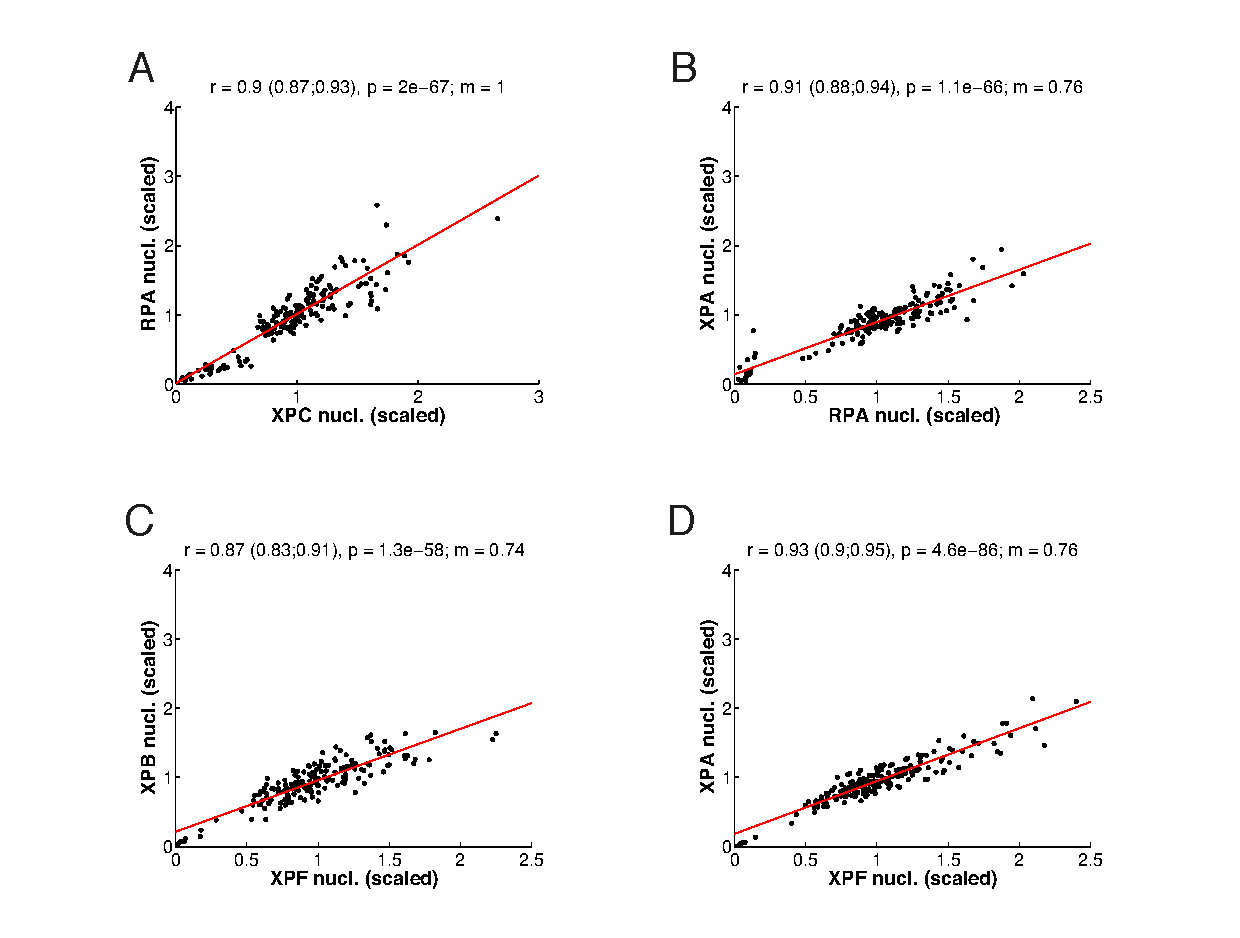
\includegraphics[width=1\textwidth]{Abbildungen/figure4_3.pdf}
%		\caption{\textbf{Blubb.} A) B) }
%		\label{fig:coExpressionData_woDamage}
%	\end{center}
%\end{figure}

\section {Cell cycle independent cross-correlation of NER factor expression}

To confirm the microscopy results we repeated the experiment by flow cytometry, this time, investigating the NER-factor expression in human brain pericytes. We established a double-staining protocol for XPA and RPA and observed that in this cell type the expression of the two repair factors also strongly correlates (cf.\ Figure \ref{fig:FC_correlation}A and B).    
\begin{figure}[htbp]
	\begin{center}
		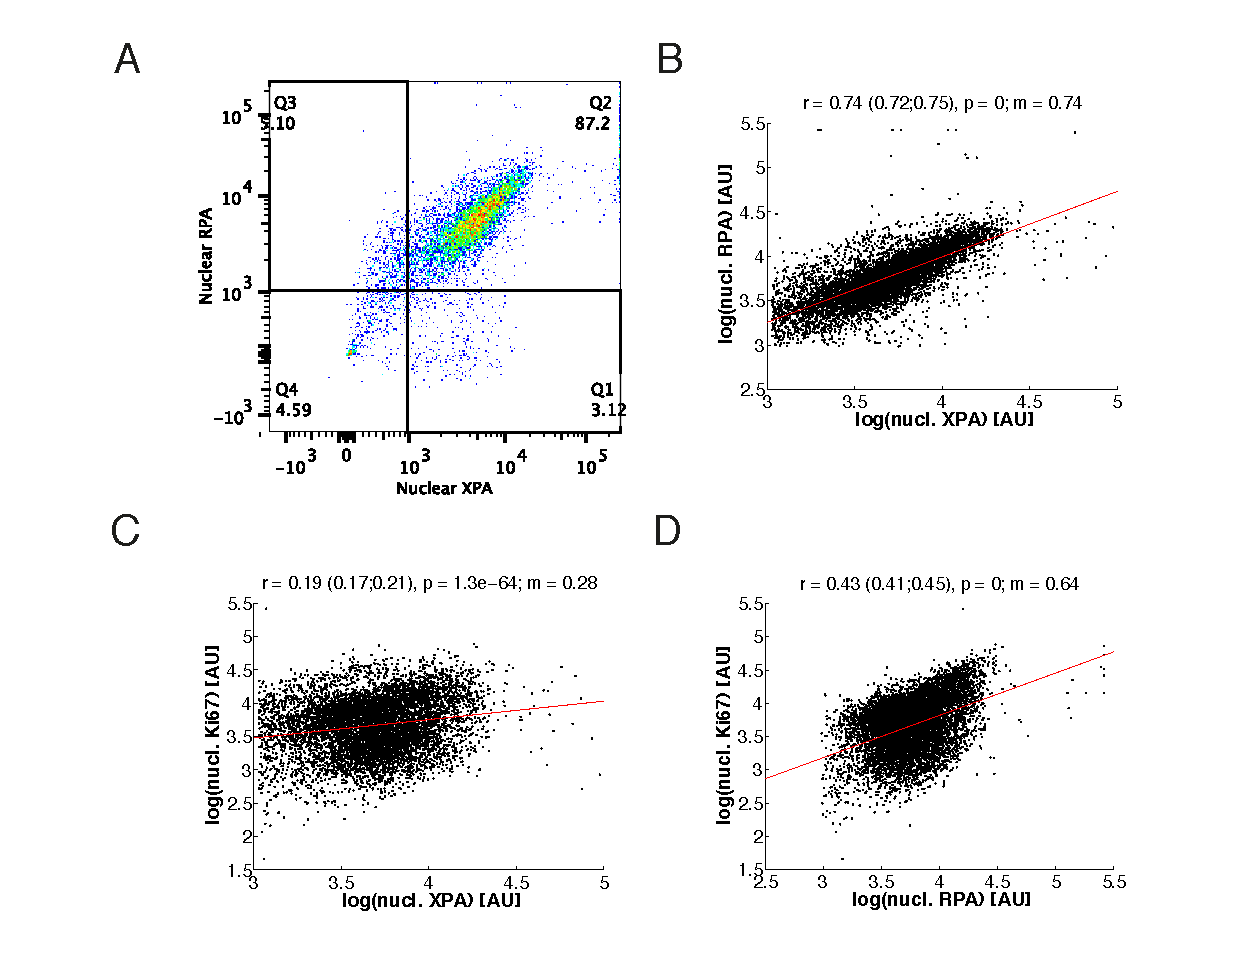
\includegraphics[width=1\textwidth]{Abbildungen/figureTAC_3.pdf}
		\caption{\textbf{Correlated expression of RPA and XPA in human brain pericytes} A) Selection of XPA and RPA positive human brain pericytes (Q2) as determined by flow cytometry (n=8084). B-D) Nuclear expression of indirectly antibody-labelled RPA against XPA (B), Ki67 against XPA (C) and Ki67 against RPA (D). B-D) Red lines represent linear regression with correlation coefficient r, p-value and slope m. 95\% confidence bounds of all correlation coeffiecients r were estimated by non-parametric bootstrap and are given in brackets.}
		\label{fig:FC_correlation}
	\end{center}
\end{figure}
Quantitatively, the correlation coefficients of the double-staining signals in both cell types have the same order of magnitude. In particular, each value falls into the confidence interval of the other (cf.\ Figure \ref{fig:FC_correlation}B and Figure \ref{fig:coExpressionData}D). To test whether this correlation is specific for proteins involved in DNA repair we measured the expression of the proliferation marker Ki67. Surprisingly, although the correlation between both repair factors and Ki67 is visibly reduced (XPA vs. Ki67 = 0.19 and RPA vs. Ki67 = 0.43 against XPA-RPA = 0.73), it is still significantly positively correlated (cf.\ Figure \ref{fig:FC_correlation}C and D).\\
As Ki67 increases during cell cycle we asked, to what extent the observed protein correlation of Ki67 and the NER factors is cell-cycle dependent. To answer this question, we stained the cell's DNA using FxCycle violet and gated them according to their DNA content (cf.\ Figure \ref{fig:FC_cell_cycle}A). Two distinct peaks denote the portion of cells traversing the G1 or the synthesis and G2 phase, respectively. By sorting the protein expression values in accordance with their cell cycle phase we identified for each protein combination two contiguous regions revealing a general trend of increased protein expression during the S1 and G2 phase in comparison to the G1 phase (cf.\ Figure \ref{fig:FC_cell_cycle}B-D).\\
Remarkably, whereas the correlation coefficients between XPA and RPA remain constant in both regimes (G1: 0.71, S+G2: 0.68, all: 0.74) the correlation between XPA and Ki67 disappear (G1: -0.072, S+G2: -0.068). Between RPA and Ki67 there is close to no correlation in the G1 phase but a significant small positive correlation in the S and G2 phase (G1: 0.12, S+G2: 0.29). These results strengthen the conclusions derived from the cross-correlation analysis in fibroblasts that NER factor expression is functionally co-regulated. In particular, the missing correlation between the nuclear factors and the cell cycle marker after taking the cell-cycle into account suggests that the measured correlation is specific to NER proteins. 




%sentence about RPA - Ki67 correlation

\section{Measured average response agrees with model prediction}
To determine potential mutual dependencies in NER factor expression we performed two independent cross-correlation experiments, firstly based on microscopy of human fibroblast and secondly using flow cytometry in human brain pericytes. For both approaches we found conclusive evidence for a positive pairwise correlation of the nuclear repair factor concentration. As described in Section \ref{sec:crossCorelResponse} the measured cross-dependencies represent the entries of matrix $B$ in Eqn. \ref{eqn:matrixNotation}. In theory, the product of the inverse of $B$ and $A$ define the vector of response coefficients. However, due to the strong multicolinearity the matrix $B$ has variance inflation factors (VIF) between 2.5 and 10.8 indicating that the variations of each protein are largely explained by a linear combinations of the other protein expression values. VIFs measure how much of the predicted standard error of the response coefficient estimates is caused by the colinearity. For instance, for a VIF of 5 the estimated error is  about $\sqrt{5} \cong 2.3$ times as large as it would be if the matrix $B$ was uncorrelated.\\ 
\begin{figure}[htbp]
	\begin{center}
		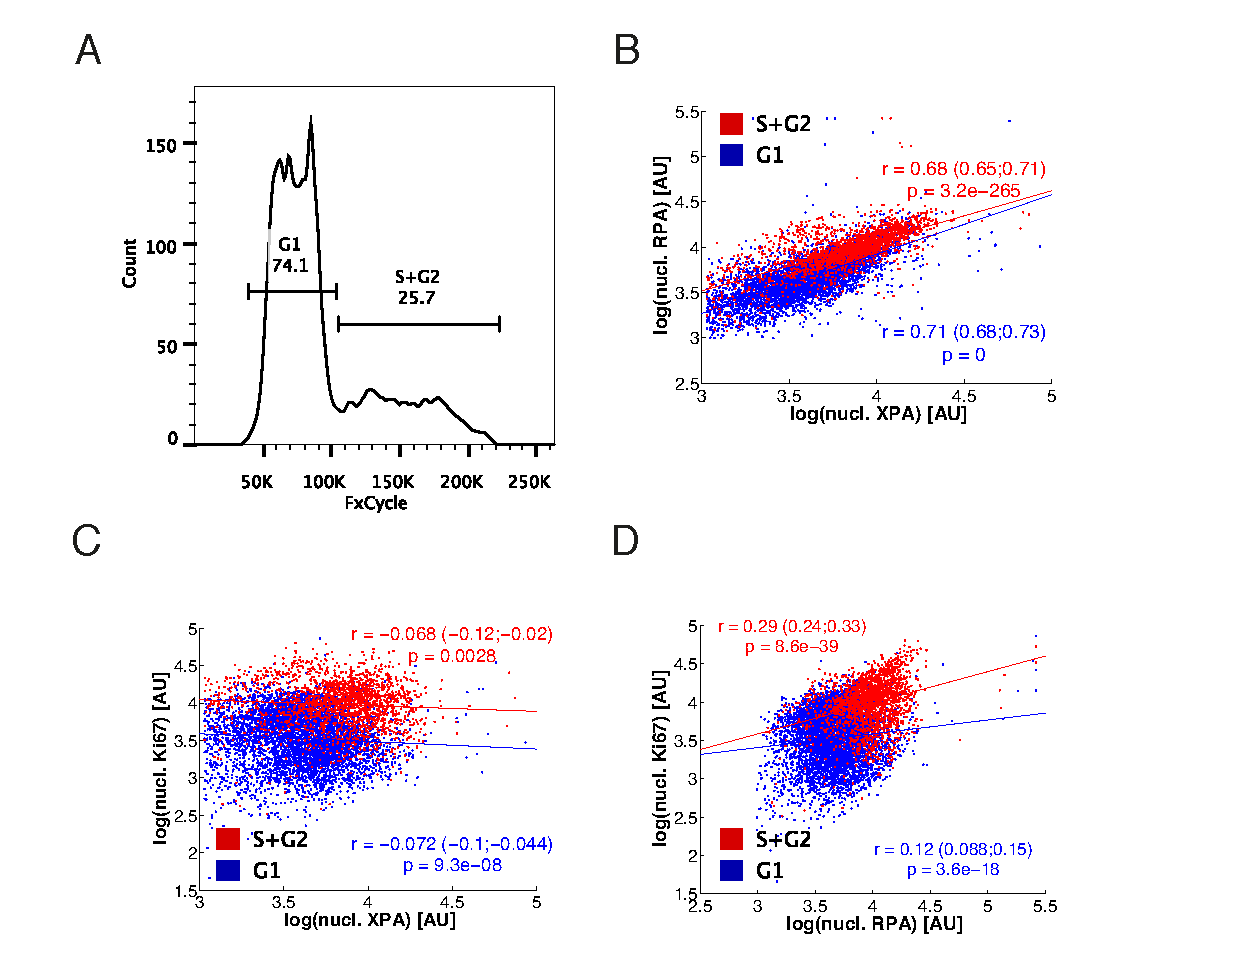
\includegraphics[width=1\textwidth]{Abbildungen/figureTAC_4.pdf}
		\caption{\textbf{NER factor cross-correlation is robust against cell cycle progression.} A) Distribution of fluorescently labelled DNA proportional to the DNA content. Horizontal bars indicate the fractions of cells assigned to G1 (left peak, n=5469) and S+G2 (right peak, n=1945).  B-D) Individual regression analysis of the nuclear expression values sorted according to the corresponding cell-cycle phase (G1 - blue; S+G2 - red) for RPA vs. XPA (B), Ki67 vs. XPA (C) and Ki67 vs. RPA (D). B-D) Red and blue lines represent linear regression with correlation coefficient r and p-value. 95\% confidence bounds of all correlation coefficients r were estimated by non-parametric bootstrap and are given in brackets.}
		\label{fig:FC_cell_cycle}
	\end{center}
\end{figure}  
Hence, we are not able to derive a reliable result for each response coefficient. However, it is possible to make an estimation of the average size of $R$. Consider $\nu$ as a function of the concentration of the repair factors $C_i$ and the initial amount of DNA lesions $L$:
\begin{equation}
	\nu = Lf(C_1,...C_N).
\end{equation}
Using, once more, the standard law for the propagation of uncertainty analogue to Eqn.\ \ref{eqn:lawoferrorPropagation}
 \begin{equation}
 \sigma(\nu) = \sqrt{\sum_{i}\left(\frac{\partial \nu}{\partial C_i}\sigma(C_i) \right)^2 + \left(\frac{\partial \nu}{\partial L}\sigma(L)\right)^2 + \left(\frac{\partial \nu}{\partial C_i} \frac{\partial \nu}{\partial C_i}\textrm{cov}_{ij}\right)^2}
 \end{equation}  
 
and introducing the response coefficients from Eqn.\ \ref{eqn:responseCoefficientsII} we derive

\begin{equation}
	CV_{\nu}^2 = CV_{L}^2 + \sum_{i}(R_iCV_i)^2 + \sum_{j\neq i} R_iR_j \frac{\textrm{cov}_{ij}}{\langle C_i \rangle\langle C_j\rangle}.
	\label{eqn:lawOfErrorPropII}
\end{equation}

With the simplifying assumption that $R = R_i$ we can solve Eqn.\ \ref{eqn:lawOfErrorPropII} for $R$ and thereby derive an estimate for the average response coefficient:

\begin{equation}
	R = \sqrt{	\frac{CV_{\nu}^2 - CV_L^2}{\sum_{i} CV_i^2 + \sum_{j\neq i} \frac{\textrm{cov}_{ij}}{\langle C_i \rangle\langle C_j\rangle}}}.
	\label{eqn:averageResponse}
\end{equation} 


On the right-hand side we measured most of the CVs and about a third of the NER factor covariations (cf.\ Table \ref{tab:proteinVariability}, Figure \ref{fig:coExpressionData} and \ref{fig:nuklearCrosscorrelation}). The missing entries were added by taking the average of the known elements. By inserting all measured and estimated quantities into Eqn.\ \ref{eqn:averageResponse} we calculated an average response coefficient of $R =$0.16. Remarkably, this result agrees exactly with the average response coefficients predicted by the model (cf.\ Figure \ref{fig:controlCoefficients}) and thus, reconfirms the hypothesis of a small and collectively shared repair-rate control.     



%hier fehlt noch klarzumachen, dass cross-correlation einen positiven Beitrag zur Variabilität vieler Zellen untereinander hat aber in einer Zelle die Variabilität der Faktoren untereinenader geringer ist




%\clearpage{\pagestyle{empty}\cleardoublepage}

% ************************* PART V *****************************

\chapter{Discussion}


Our DNA-repair analysis was made possible by the ability to explicitly observe the kinetics of resynthesised DNA during nucleotide-excision repair (NER). The quantification of this repair intermediate by following the incorporation of fluorescently labelled nucleotides on the single cell level shows that the repair process follows a slow, first-order kinetic (\textit{cf.}\ Chapter \ref{chap:quantData}). These new data supplement comprehensive fluorescent real-time measurements quantifying the dynamic behaviour of single repair proteins. Hence, we can observe the individual protein exchange kinetics at the chromatin fibre, which eventually lead to the formation of catalytic multi-protein machineries, concomitantly with the global repair process. Based on this information we were able to identify a detailed kinetic model of NER, which allows us to establish a quantitative link between fast and random assembly of the NER factors at the DNA template and the emergent phenomenon of a slow overall repair time (\textit{cf.}\ Chapter \ref{chap:kineticNERmodel}). The most important implication of the model is that the repair rate is controlled by the repair factors in a collective way. In particular, the uniformly small response coefficients emphasize the robustness of the DNA repair process. This disproves the widely-held assumption that a single rate-limiting step controls the entire repair process \cite{Hoogstraten2008,Koberle2006,Kang2011}. Our theory of a shared control has been corroborated qualitatively by exploiting experimental measurements of the natural variability of the nuclear NER factor concentrations (\textit{cf.}\ Chapter \ref{chap:robustRepair}). However quantitatively, the measured repair responses exceed the magnitude of the predicted response coefficients significantly.\\
While further pursuing the nature of the measured cell-to-cell variability and its influence on DNA repair, we observed that the substantial heterogeneity of the repair rate is generated primarily by the distribution of inflicted DNA lesions. This factor is complemented by the variability contributed from the nuclear concentration of each individual repair factor. The quantitative impact of these two parameters on the cell-to-cell variability of DNA repair is consistent with the robustness of the repair rate against concentration fluctuations of individual repair factors (\textit{cf.}\ Chapter \ref{chap:robustRepair}).\\  
Interestingly, we also found evidence for the regulated NER factor expression indicated by strong cross-correlations of the protein concentrations. Considering these mutual interdependencies in our control analysis quantified their contribution to the repair-rate response and thus, explains the gap between measured and predicted DNA repair response (\textit{cf.}\ Chapter \ref{chap:crossCorell}). These results imply that the robustness of the repair rate is not only controlled by the pathway-intrinsic molecular interplay of chromatin-associated machineries but also extrinsically by a regulatory mechanism orchestrating NER factor expression.\\
In the following, we will elaborate a more detailed discussion about individual findings including: The DNA repair kinetics, NER model identifiability, model parametrization, repair-rate control and the co-regulation of NER factor expression.     
% * <l.adlung@dkfz.de> 2014-12-10T23:05:46.669Z:
%
%  Regarding collective control: Do you mention at any point the phenotype of knockouts of the individual repair factors? I remember that you indicating it when speaking about knock down or overexpression...
%

\paragraph{Slow first order kinetics as a general systems property for chromatin associated processes}
In our analysis of the NER kinetic we focused on the removal of one of the major UV-induced DNA lesions, the 6-4 pyrimidine-pyrimidone photoproducts (6-4PPs) (\textit{cf.}\ Figure \ref{fig:DNArepairKinetic}B), which are repaired significantly faster ($\sim$2-3 hours) compared to cyclobutane-pyrimidine dimers (CPDs), for which the majority is still present after $\sim$24 hours \cite{Smerdon1978,vanHoffen:1995:EMBO-J:7835346,Luijsterburg2010}. 6-4PPs are repaired by incision of the damaged DNA strand, and subsequent DNA resynthesis, which we were able to monitor by following the incorporation of the fluorescently tagged thymidine analogue EdU. The nucleotides are labelled by copper-catalysed covalent addition of the fluorophore, which requires the cells to be fixed. Hence, EdU accumulation cannot be measured continuously in one cell. Instead, we followed EdU incorporation stepwise by permeabilising cells after increasing time intervals, each starting immediately after UV-irradiation. In this way we were able to show that the 6-4PP repair fits to a first order kinetic with a half-time of $\sim$1.2 hours.         
This long time-scale is in contrast to the rapid exchange behaviour of early and late repair factors as reported by several live-cell imaging studies. \cite{Houtsmuller1999,Volker2001,Hoogstraten2002,Rademakers2003,Mone2004,Zotter2006,Hoogstraten2008,Luijsterburg2010}. \\
%Recently, these results could be generalized for all core NER factors combining different photobleaching and fluorescence life-time microscopy approaches \cite{}.The work in this thesis strengthens a prominent explanation of this time-scale contradiction using the comprehensive biological knowledge about NER together with mathematical modelling.\\
In agreement with a simplified model simulating the assembly of a catalytic protein repair-complex \cite{Terstiege2010}, we find here that reversible exchange of NER factors is the key property that makes NER an apparent first-order process. In this description, the long time-scale arises from the concurrence of stochastic assembly and reversible exchange of the constituent components, which leads to the formation of many non-functional preliminary stages before eventually the catalytic complex is completed. This is in contrast to a sequence of irreversible binding steps, which will create sigmoidal kinetics with an even sharper delay with increasing numbers of assembling components \cite{Terstiege2010}. As suggested by Luijsterburg \textit{et al.} (2010) \cite{Luijsterburg2010}, the slow repair time might actually present an advantage for the specificity of the repair process, analogous to a kinetic proof-reading mechanism, where differential dissociation kinetics would prevent false-positive lesion detection. \\ 
The phenomenon of rapid protein exchange is widespread also in other chromatin associated processes such as replication, chromatin remodelling or transcription \cite{McNairn2005,Erdel2011,Sonneville2012,Stasevich2011}. Analogous to NER, these processes involve finding a specific reaction site before the catalytic machinery can assemble at the same location. In the particular case of DNA transcription, transient protein dynamics were experimentally demonstrated for transcription factor binding and transcription machinery assembly \cite{Hager2009}. The time scales for these reactions (several seconds to minutes) are comparable to our results for DNA repair. This encourages us to hypothesise that the slow time scales of transcriptional bursting in mammalian cells (tens of minutes to hours; \cite{Harper2011,Suter2011}) also arise through the reversible assembly of large macromolecular complexes.   



\paragraph{A predictive kinetic model of DNA repair}
Augmenting the extensive kinetic data on binding and dissociation of individual components of the NER machinery \cite{Luijsterburg2010} with a direct readout for DNA repair synthesis, we were able to develop a predictive ODE-model of NER (\textit{cf.}\ Chapter \ref{chap:kineticNERmodel}). To the best of our knowledge it is the first model of a DNA-associated process, for which the model parameters could be identified (\textit{i.e.}, parameter values uniquely assigned with narrow confidence bounds) from experimental data. \\
On the technical side, to make the profile likelihood estimation for each parameter computationally feasible, we first needed to optimize the runtime of the parameter estimation algorithm. Therefore, we integrated the model into a dynamic modelling framework that applies a deterministic trust-region fitting algorithm implemented in MATLAB \cite{Raue2009}. The accuracy and computational performance of the implementation benefit immensely from the simultaneous integration of the dynamic variables concomitantly with the derivatives of the objective function with respect to the model parameters \cite{conn2009introduction,Ramachandran2010,Raue2013}. Solving this extended system of ordinary differential equations with a CVODE solver implemented in C accelerated the speed for one deterministic optimization run by 200-fold compared to the previously applied stochastic Markov Chain Monte Carlo (MCMC)\label{sec:MCMC} optimization algorithm \cite{Terstiege2010}. The runtime spent for one fit on a 12-core processor with 3 GHz each is now reduced from two weeks to $\sim$10 minutes. This considerable runtime improvement allowed us to sample the parameter space exhaustively using Latin hypercube sampling, a technique, which makes the deterministic optimization algorithm more robust against local optima \cite{Raue2013}.\\
In addition to fitting the parameters that determine the model dynamics, we estimated the parameters that characterize the measurement noise. This approach of explicitly including the measurement noise, has the advantage that it avoids an inaccurate \textit{ad hoc} estimate of the experimentally-determined error due to low numbers of replicates and thus gives a more exact assessment of the model parameters, without preprocessing the experimental data \cite{Raue2013}. \\
Imposed by the non-identifiability of several parameters in the model of Luijsterburg \textit{et al.} \cite{Luijsterburg2010}, a number of simplifications concerning the model structure were required to achieve an identifiable model of the NER pathway. The two most significant modifications that we introduced here are the removal of the 'partially unwound' repair intermediate and the neglect of protein-protein interactions, in particular the sequential binding of XPA and XPF \cite{Volker2001}, for which there was no evidence in the data. Since we lack a direct readout for incised DNA, we additionally assumed a practically instantaneous incision of the DNA lesion once the pre-incision complex has been completely assembled. The missing information about DNA incision also limits the identifiability of the other catalytic rates (despite the rate of rechromatinisation), indicated by the existence of lower confidence bounds, only. This case of structural non-identifiability proved to be without consequence for the goodness of the model predictions (\textit{cf.}\ Figure \ref{fig:controlCoefficients}). Moreover, fast catalytic rate constants agree with a recent direct measurement in bacteria where DNA synthesis and ligation take seconds \cite{Uphoff2013}. \\
Our current model, whose structure is reconcilable with the experimental data, constitutes a concrete improvement over previous NER models \cite{Luijsterburg2010,Politi2005,Kesseler2007}. We believe that, gaining further mechanistic understanding about system properties requires an intertwined advancement, where the addition of molecular detail in the model is consecutively balanced by appropriate quantitative measurements. Already at the present level of detail, we are confident that the general dynamic behaviour of the model (\textit{e.g.} repair rate, robustness against protein-expression noise and fidelity of lesion recognition) will prove robust with respect to such a development as we observed these properties already for a simplified model of repair (\textit{cf.}\ Figure \ref{fig:reactionTiming} \cite{Verbruggen2014}).    
       

\paragraph{Model parametrization and its implications}
The model fit (described in detail in Chapter \ref{chap:kineticNERmodel}) yields biochemically plausible estimates for the kinetic parameters of the individual assembly and dissociation kinetics \textit{in vivo}, which account for both the long-term accumulation and for the rapid exchange of the NER factors. Notably, the affinity of the lesion recognition factor XPC is remarkably low, which is mainly caused by the high off-rate. This is consistent with previous work where high molecular off-rates have been described as a general property of self-organizing systems, which allows for efficient exploration of an assembly landscape and selection of a functional steady state \cite{Kirschner2000}. As discussed in depth at Luijsterburg and coworkers (2010)\cite{Luijsterburg2010} the strong reversibility is also beneficial for the specificity and regulation of the system, for example by preventing the trapping of NER proteins in incomplete (and thus unproductive) repair complexes. The reversibility advantage also applies for the trade-off between specificity and efficiency of the mechanism, which equally plays a role in chromatin remodelling and transcription \cite{Cook2010,Voss2011}.\\
Apart from fast reversible assembly/dissociation, parameter estimation also revealed that the catalytic rate constants are fast, which indicates a tight coupling between lesion excision and repair synthesis. This in turn implies that the lesions are repaired without much delay immediately after their recognition by XPC, which consequently prevents the accumulation of incised DNA. Our \textit{in-vivo} finding stays in contrast to \textit{in-vitro} experiments that have found a delay before repair synthesis \cite{Mocquet2008,Riedl2003}. Our prediction that the repair system prevents single-stranded repair intermediates to accumulate corresponds with our expectation that an elevated abundance of incised DNA would trigger DNA degradation to avoid the risk of an inflammatory response, autoimmunity \cite{Takeuchi2010} or simply their collapse to double strand breaks \cite{Mocquet2008}.             



\paragraph{Collective control of the DNA repair rate}
A consequence of the NER model architecture, which describes the sequential organization of this chromatin-associated process by cycles of protein recruitment, is the absence of any rate-limiting factor for repair synthesis. Instead, the control of the repair speed is homogeneously distributed, with small contributions from each repair factor. This central result of our work agrees with the outcome of previous flux control analyses of various biochemical pathways that found no experimental support for the existence of a unique rate-limiting factor \cite{Fell1992,Bruggeman2007,Yi2000a}. Moreover, response coefficients with values much smaller than 1 indicate that DNA repair is robust  against natural fluctuations of the protein concentrations in the cell \cite{Bluthgen2013}. It is important to note that the degree of control as a kinetic property of a particular NER factor is independent of its position in the order of engagement in the repair process. Thus, the lesion recognition factor XPC, which binds first, has the same control as XPA or RPA that bind much later to protect the unwound DNA single-strands.\\
As a biochemical network can never be insensitive against all possible perturbations \cite{Bluthgen2013,Csete2002}, DNA repair will be affected by larger fluctuations in the concentration of NER factors. In this respect, the model predicts that the rate of repair eventually drops to zero in case of a strong concentration reduction of any repair factor (\textit{cf.}\ Figure \ref{fig:R_largeProteinVariation}). This agrees with various studies showing that a significant reduction in nuclear XPC and XPA levels leads to decreased cell survival and/or decreased lesion removal \cite{Koberle1999,Koberle2006,Renaud2011}. In contrast, increased levels of ERCC1 and XPA lead to increased resistance in certain tumours against cisplatin, which induces DNA interstrand crosslinks specifically removed by NER \cite{Koberle1999,Koberle2006,Renaud2011,Stewart2007,Arora2010}.   
\\ 
To analyse the effect of natural changes in NER factor expression on the repair rate experimentally, instead of changing the protein expression by gene knock-down or overexpression, which usually cause the partial or complete disruption of essential system functions \cite{Moriya2006}, we exploited the natural variability of the nuclear protein concentration. Despite the weak correlation in the data, we saw a significantly positive dependency between protein expression for all five measured NER factors and DNA resynthesis (\textit{cf.}\ Figure \ref{fig:Nuc_vs_DNAsynthesis}). The regression slopes were evenly distributed and below unity, which corroborates the finding of a shared moderate repair-rate control.\\  
Not surprisingly, there are studies indicating that the collective control of a systems property (\textit{e.g.} repair rate) is not an exclusive concept for the DNA repair pathway, but also applies to other chromatin-associated processes. For example, it was shown that the probability to express interferon-$\beta$ was significantly increased, when five out of six transcription factors necessary for transcriptional activation were overexpressed \cite{Apostolou2008}. A similar result was obtained recently, which suggested that the expression of of IL-2 is induced by the concerted interplay of four transcription factors together with FOXP3 \label{sec:FOXp3} \cite{Bendfeldt2012}. These findings emphasize that also transcription is a collectively controlled process.   

% * <l.adlung@dkfz.de> 2014-12-10T23:28:41.870Z:
%
%  Are those collective overexpression results always compared to single overexpression?
%
%Each cell is exposed to many strong perturbations on

\paragraph{Co-regulation of the nuclear NER factor expression}    The question how robustness to perturbations of the cellular state emerges from the underlying biochemical networks, has attracted considerable interest. A range of regulatory motifs have been proposed as producers of a robust response (\textit{e.g.} negative feedback, incoherent feed-forward loops and functional redundancy) \cite{Alon2007,Bleris2011,Yi2000,Manuscript2011}. However, most of these functional building blocks are not applicable for promoting robust DNA repair as the NER pathway shows robust regulation without any reported signalling events (as described in this work), nor should transcriptional regulation play a role on the considered time scale between damage infliction and repair initiation \cite{Mone2001}. The individual repair reactions purely depend on the repair complex assembly time and thus are determined by the NER factor binding affinities (this work and \cite{Luijsterburg2010}). In essence, robustness of the repair speed relies on the fact that minor delays or speed-ups caused by fluctuations of one repair factor during the assembly process of the full complex, are negligible on the global time scale. Therefore, randomness in many reversible steps is averaged by the law of large numbers. In this way the robustness of DNA repair is directly linked to the dynamic design of the repair pathway.\\     
Intriguingly, we found experimental evidence for the regulated expression of the NER factors themselves, indicated by a strongly positive pairwise correlation for all seven measured repair factor combinations. In contrast to previous studies showing correlated mRNA \label{sec:mRNA} levels for different NER factors in cancers cells \cite{Damia1998,Cheng2000}, we observed this cross-correlated expression in single cells of various types under unperturbed, NER-independent conditions. Despite the overall increase in nuclear NER factor concentrations during S-phase and G2 phase, the cross-correlation persists independently of the cell cycle. Together, these results imply an additional regulative mechanism that indirectly controls the repair rate already on the transcriptional level. Since, as we show, NER control is distributed, we predict that this transcriptional control must act on many factors simultaneously to be effective.\\
Remarkably, the co-expression of NER factors has strong conceptual similarity to bacterial signal transduction systems, where different regulatory enzymes are encoded on the same operon \cite{Kollmann2005,Lovdok2009}. This co-localisation leads to co-expression, which in turn provides concentration robustness against variability of other pathway components \cite{Bluthgen2013}. So far such a transcriptional coupling mechanism is unknown for the repair proteins involved in NER. Therefore it would be interesting to investigate whether this co-expression can be perturbed pre-transcriptionally to further study its impact on the rate of repair. 

% * <l.adlung@dkfz.de> 2014-12-10T23:33:35.858Z:
%
%  Perturbation in the sence of mono-cistronic mRNA?
%
% ^ <l.adlung@dkfz.de> 2014-12-10T23:36:20.513Z:
%
%  Is there any RNAseq data to corroborate correlated mRNA levels for the NER factors?
%

\paragraph{Concluding remarks}
The accurate repair of DNA is essential for the long-term survival of the cell since it is absolutely necessary for the fidelity of all chromatin-associated processes. It is therefore not surprising to find two molecular cooperating mechanisms that ensure robustness of the repair rate against natural variability. First, as a consequence of the dynamic design of the repair complex assembly, there exists a uniformly distributed control of the repair rate, where each factor has only a moderate effect on its own. This translates into a low system response in the event of fluctuations of the NER factor concentrations. Second, a yet unknown extrinsic mechanism regulates the coordinated NER factor expression, which limits the degree of protein variability, presumably, already pre-transcriptionally. Given that chromatin remodelling, transcription and translation have similar dynamic features as DNA repair, both mechanisms may function as a widespread mode of robust regulation of chromatin-associated processes. 


%- was passiert am Anfang wenn Chromatin remodeled wird...;was passiert, wenn zusätzliche Schritte mit einbezogen werden; was ist generell wichtiger für die Zelle - eine schnelle Reparatur oder, dass der Prozess robust ist...; eine langsame Reparatur ermöglicht natürlich auch Kinetik proofreading; wie anfällig ist der Prozess von korrekter Chromatin Remodulierung? Talk about that this is a leap forward that we directly measure DNA synthesis 

%wie kann man das Transkriptionsgefüge destabilisieren... Findet die Regulation der Proteinkonzentration vor oder nach dem ablesen statt? Is there any RNAseq data? mono-cistronic DNA 

%\clearpage{\pagestyle{empty}\cleardoublepage}


% ************************* PART VI *****************************
%\include{chapters/MaterialsandMethods}

%\thispagestyle{empty}
%\clearpage{\pagestyle{empty}\cleardoublepage}


%\thispagestyle{empty}
%\clearpage{\pagestyle{empty}\cleardoublepage} \pagestyle{fancy}
%\lhead[\normalsize\thepage\hfill\footnotesize\leftmark\ ]{} \chead{}
%\rhead[]{\footnotesize\rightmark\hfill\normalsize\thepage} \lfoot{}
%\cfoot{} \rfoot{}




% ************************* Publications *****************************

%\include{chapters/Publications}
%\clearpage{\pagestyle{empty}\cleardoublepage} \thispagestyle{empty}
%\clearpage{\pagestyle{empty}\cleardoublepage}

% ************************* List of Figures *****************************
%\addcontentsline{toc}{chapter}{List of Figures}
%\listoffigures \clearpage{\pagestyle{empty}\cleardoublepage}

% ************************* References *****************************
%\setcounter{chapter}{9}
%\addcontentsline{toc}{chapter}{Bibliography}
%\bibliographystyle{apa}
%\newcommand{\bibfont}{\footnotesize}
\footnotesize\bibliographystyle{naturemagC}
\bibliography{NER_Bibliography}

%\clearpage{\pagestyle{empty}\cleardoublepage} \thispagestyle{empty}
%\clearpage{\pagestyle{empty}\cleardoublepage}


%\clearpage{\pagestyle{empty}\cleardoublepage} \thispagestyle{empty}
%\clearpage{\pagestyle{empty}\cleardoublepage}

% ************************* Appendix *****************************

\appendix
\chapter{Appendix}
\pagestyle{plain4}
\setcounter{table}{0}
\renewcommand{\thetable}{A\arabic{table}}

\section{Parameter estimation}


\begin{figure}[h!]
\begin{center}
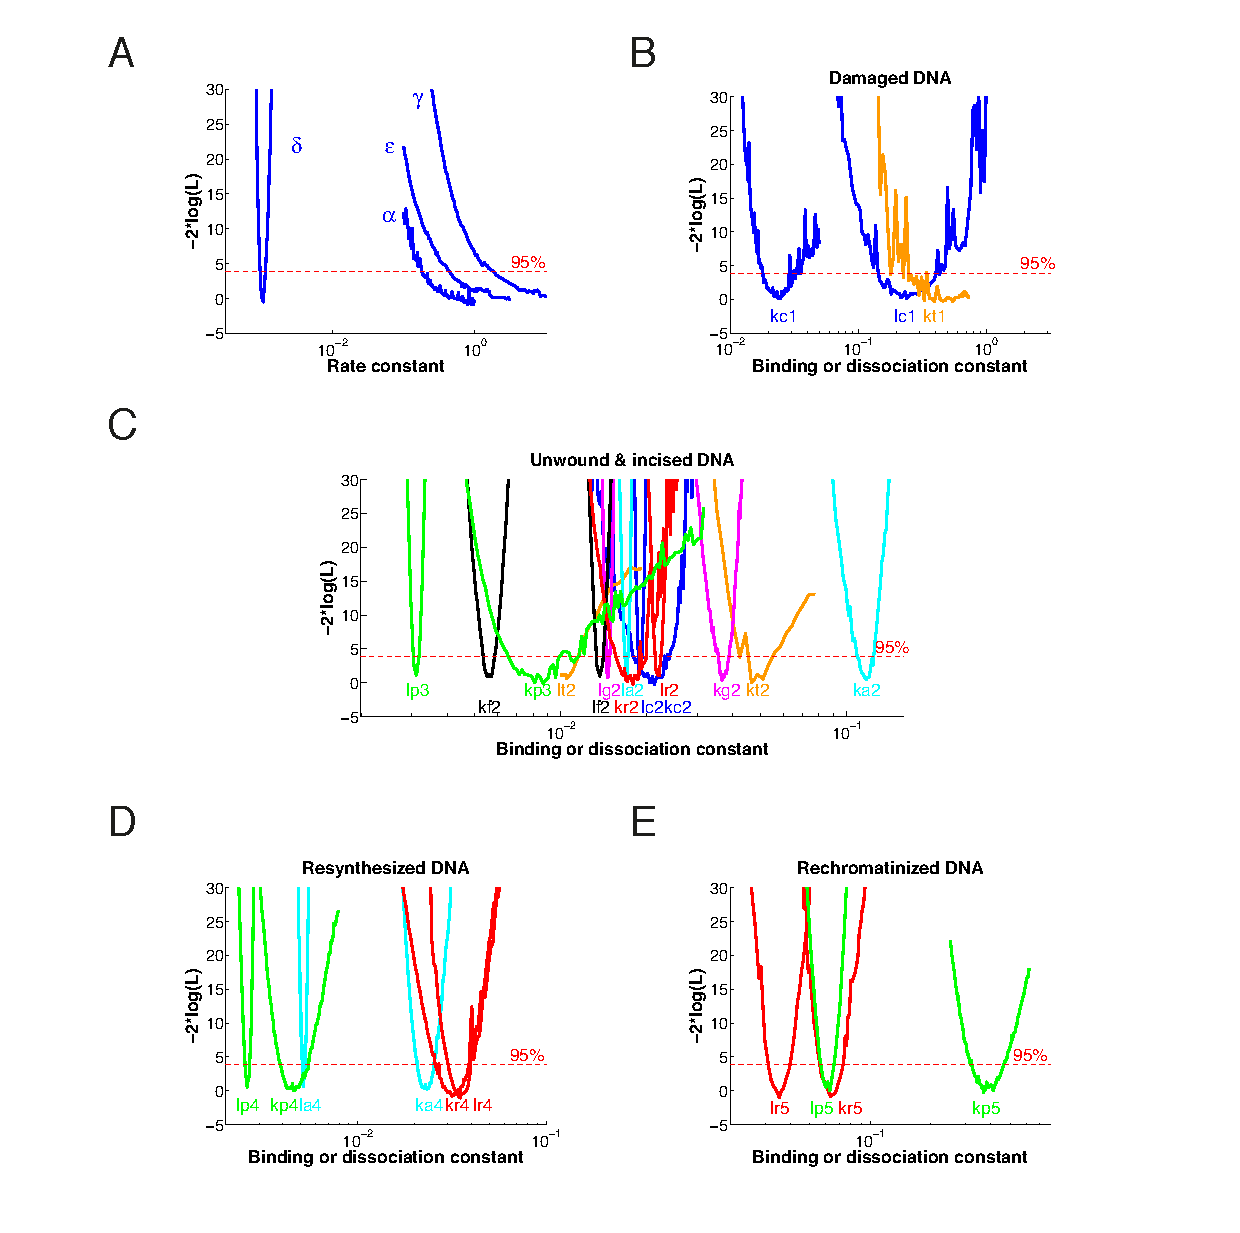
\includegraphics[width=1\textwidth]{Abbildungen/figure_A_1.pdf}
\caption{\textbf{Identifiability analysis by profile likelihood estimation (PLE).} PLE and 95\% confidence limit (horizontal red line) of binding and dissociation parameters for A) all catalytic constants, B) damaged DNA, C) unwound and incised DNA, D) resynthesised DNA and E) rechromatinised DNA. }
\label{fig:profileLikilihoods}
\end{center}
\end{figure}

\begin{table}[H]
	
	\tiny
	\begin{tabular}{lccccccc}
		
		\multicolumn{8}{l}{} \\
		\hline
		\textbf{Value}    & \textbf{ XPC} & \textbf{TFIIH} & \textbf{XPG} & \textbf{XPF} & \textbf{XPA} & \textbf{RPA} & \textbf{PCNA}  \\
		\hline
		Concentration ({\textmu}M)                                                                        &0.140    & 0.360 & 0.440& 1.110& 0.170& 1.110& 1.110     \\
		\multicolumn{8}{l}{\textbf{Damaged DNA}} \\
		$\text{k}_{\text{on}}$({\textmu}$\text{M}^{\text{-1}}\text{s}^{\text{-1}})$& 0.025               & 0.2  & NA &NA&NA&NA&NA     \\
		& (0.013;0.036)     & (0.152;0.288)  &&&&&   \\
		$\text{k}_{\text{off}}$($\text{s}^{\text{-1}})$                                             & 0.231                & 0.01 & NA &NA&NA&NA&NA     \\
		& (0.136;0.36)     &(0.009;0.012)  &&&&&   \\
		$\text{K}_{\text{d}}$({\textmu}$\text{M})$                                                  & 9.35                & 0.052  & NA &NA&NA&NA&NA     \\
		& (3.46;16.09)     &(0.044;0.072)  &&&&&   \\
		\multicolumn{8}{l}{\textbf{Unwound DNA}} \\
		$\text{k}_{\text{on}}$({\textmu}$\text{M}^{\text{-1}}\text{s}^{\text{-1}})$    & 0.022                     & 0.049                   & 0.037                 &  0.0056             & 0.116                   &0.018                    & NA    \\
		& (0.016;0.025)     & (0.04;0.06)   					&(0.036;0.039) 		 & (0.0054;0.0059)&(0.109;0.125)    &(0.016;0.02)    &     \\
		$\text{k}_{\text{off}}$($\text{s}^{\text{-1}})$                                             & 0.019                     & 0.01                   & 0.0146               & 0.0137                & 0.017                   & 0.022                   &NA     \\
		& (0.019;0.019)     & (0.009;0.012)             & (0.0140;0.0149)&(0.0134; 0.0141)&(0.0167;0.0172)     &  (0.0213;0.0224)  &   \\
		$\text{K}_{\text{d}}$({\textmu}$\text{M})$                                                  & 0.864                     & 0.204                   & 0.395                 &2.446                 &0.147                    &1.222                    &NA     \\
		& (0.635;1.006)     & (0.163;0.259)             & (0.373;0.419)		&(2.344; 2.596)&(0.138;0.158)     &  (1.048;1.36)  &   \\
		\multicolumn{8}{l}{\textbf{Incised DNA}} \\
		$\text{k}_{\text{on}}$({\textmu}$\text{M}^{\text{-1}}\text{s}^{\text{-1}})$    & 0.022                     & 0.049                   & 0.037                 &  0.0056             & 0.116                   &0.018                    & 0.008    \\
		& (0.016;0.025)     & (0.04;0.06)   					&(0.036;0.039) 		 & (0.0054;0.0059)&(0.109;0.125)    &(0.016;0.02)    	& (0.0066;0.0111)    \\
		$\text{k}_{\text{off}}$($\text{s}^{\text{-1}})$                                              & 0.019                     & 0.01                   & 0.0146               & 0.0137                & 0.017                   & 0.022                 &0.0031     \\
		& (0.019;0.019)     & (0.009;0.012)             & (0.0140;0.0149)&(0.0134; 0.0141)&(0.0167;0.0172)     &  (0.0213;0.0224)    & (0.003;0.0032)  \\
		$\text{K}_{\text{d}}$({\textmu}$\text{M})$                                                   & 0.864                     & 0.204                   & 0.395                 &2.446                 &0.147                    &1.222                   &0.388    \\
		& (0.635;1.006)     & (0.163;0.259)             & (0.373;0.419)		&(2.344; 2.596)&(0.138;0.158)     &  (1.048;1.36)  					& (0.319;0.538)   \\
		\multicolumn{8}{l}{\textbf{Resynthesised DNA}} \\
		$\text{k}_{\text{on}}$({\textmu}$\text{M}^{\text{-1}}\text{s}^{\text{-1}})$    & NA                          & NA                        & NA                      &  NA                    & 0.022                   &0.032                    &0.004    \\
		&                               &                             &                            &                          &(0.021;0.025)    &(0.025;0.037)    & (0.0038;0.005)    \\
		$\text{k}_{\text{off}}$($\text{s}^{\text{-1}})$                                             & NA                          &NA                          & NA                      & NA                     & 0.0052                  & 0.035                   &0.0026     \\
		&                               &                              &                           &                          &(0.0051;0.0053)     &  (0.031;0.042)  & (0.0025;0.0027)  \\
		$\text{K}_{\text{d}}$({\textmu}$\text{M})$                                                  & NA                          &NA                         & NA                      &NA                      &0.236                   &1.167                    &0.605     \\
		&                               &                              &                           &                          &(0.222;0.27)     &  (0.924;1.521)  & (0.531;0.747)  \\
		\multicolumn{8}{l}{\textbf{Rechromatinised DNA}} \\
		$\text{k}_{\text{on}}$({\textmu}$\text{M}^{\text{-1}}\text{s}^{\text{-1}})$    & NA                          & NA                        & NA                      &  NA                    & NA                       &0.065                    &0.396    \\
		&                               &                             &                            &                          &                            &(0.056;0.075)    & (0.359;0.457)    \\
		$\text{k}_{\text{off}}$($\text{s}^{\text{-1}})$                                             & NA                          &NA                          & NA                      & NA                     & NA                       & 0.035                   &0.061     \\
		&                               &                              &                           &                          &                            &  (0.031;0.04)  & (0.056;0.067)  \\
		$\text{K}_{\text{d}}$({\textmu}$\text{M})$                                                  & NA                          &NA                         & NA                      &NA                      &NA                         &0.538                    &0.154     \\
		&                               &                              &                           &                          &                            &  (0.438;0.645)  & (0.134;0.182)  \\
		\hline
	\end{tabular}
	\caption{\textbf{Values of binding and dissociation rate constants.} NA, not applicable. $k_{\text{on}}$, $k_{\text{off}}$ and $\text{K}_{\text{d}}$ ($k_{\text{off}}$/$k_{\text{on}}$) values are given for every repair protein and arranged in columns. Reference parameter set and 95\% confidence intervals (in parentheses) are shown. Nuclear concentration (in \textmu M) of NER factors are based on previously described data \cite{Luijsterburg2010}}
	\label{tab:parameter_bigTable}
\end{table}

\begin{table}[H]
	
\begin{center}
	\begin{tabular}{lrl}
		
		\multicolumn{3}{l}{} \\
		\hline
		\textbf{Catalytic rate}    && \textbf{$\text{k}_{\text{cat}}$ $\, \left[\text{s}^{\text{-1}}\right]$}  \\
		\hline
		Unwinding  $\alpha$                                     & 19.9& (>0.2)                 \\
		Resynthesis $\gamma$                                 & 25.5 &(>1.5)     \\
		Rechromatinisation $\delta$                         & 0.001 &(0.001;0.0011)                   \\
		Reannealing  $\epsilon$                                & 5.3&(>0.9)    \\
		\hline
	\end{tabular}
	\caption{\textbf{Values of the catalytic rate constants.}  Reference parameter set and 95\% confidence intervals (in parentheses) are shown. In case of practical non-identifiability only the lower confidence bound is given.}
	\label{tab:parameter_catalyticRates}
	\end{center}
\end{table}


\section{Correlation analysis}
\label{apendix:correlationAnalysis}
The correlation analysis was performed in MATLAB (2012a, The Mathworks Inc., Natick, MA) using the inbuilt 'corrcoef' function, which also returns p-values indicating the significance of the correlation coefficient. The p-values are determined by a t-test, where the null-hypothesis $H_0$ states that the true correlation $p_r$ between two variables equals zero $H_0: \, p_r=0$ (whereas the alternative hypothesis states $H_1: \, p_r\neq0$) and that for its observed value $r$ the quantity 
\begin{equation}
t = \frac{r}{\sqrt{\frac{(1-r^2)}{N-2}}}
\end{equation}     
follows approximately a $t$-distribution for $N$ - 2 degrees of freedom and a sample size $N$ \cite{Kendall1979,Fisher1958}. A low p-value suggests the rejection of the null-hypothesis and thus, demonstrates the significance of the correlation.\\
The confidence intervals for each correlation coefficient were estimated by non-parametric bootstrap \cite{Efron1979}. Thereby the correlation coefficient was re-sampled for 10,000 times each time drawing $n$ pseudoreplicates (with replacement), where $n$ denotes the number of measured cells from the original data. The confidence borders mark the interval including 95\% of the re-sampled correlation coefficients.\\ 

\section{Control analysis}

\begin{figure}[h!]
	\begin{center}
		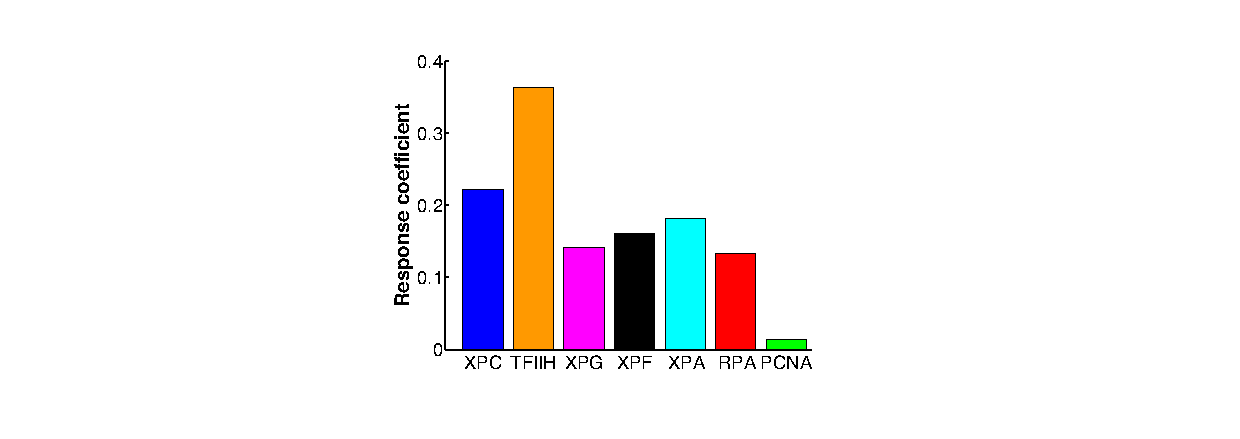
\includegraphics[width=1\textwidth]{Abbildungen/figure_A_4.pdf}
		\caption{\textbf{Uniformly distributed response coefficients for the rate of incision.} Response coefficients for the control of the incision rate by the concentrations of the repair factors. }
		\label{fig:cc_rateOfincision}
	\end{center}
\end{figure}


\newpage
\section{Cross-correlation}

\begin{figure}[h!]
	\begin{center}
		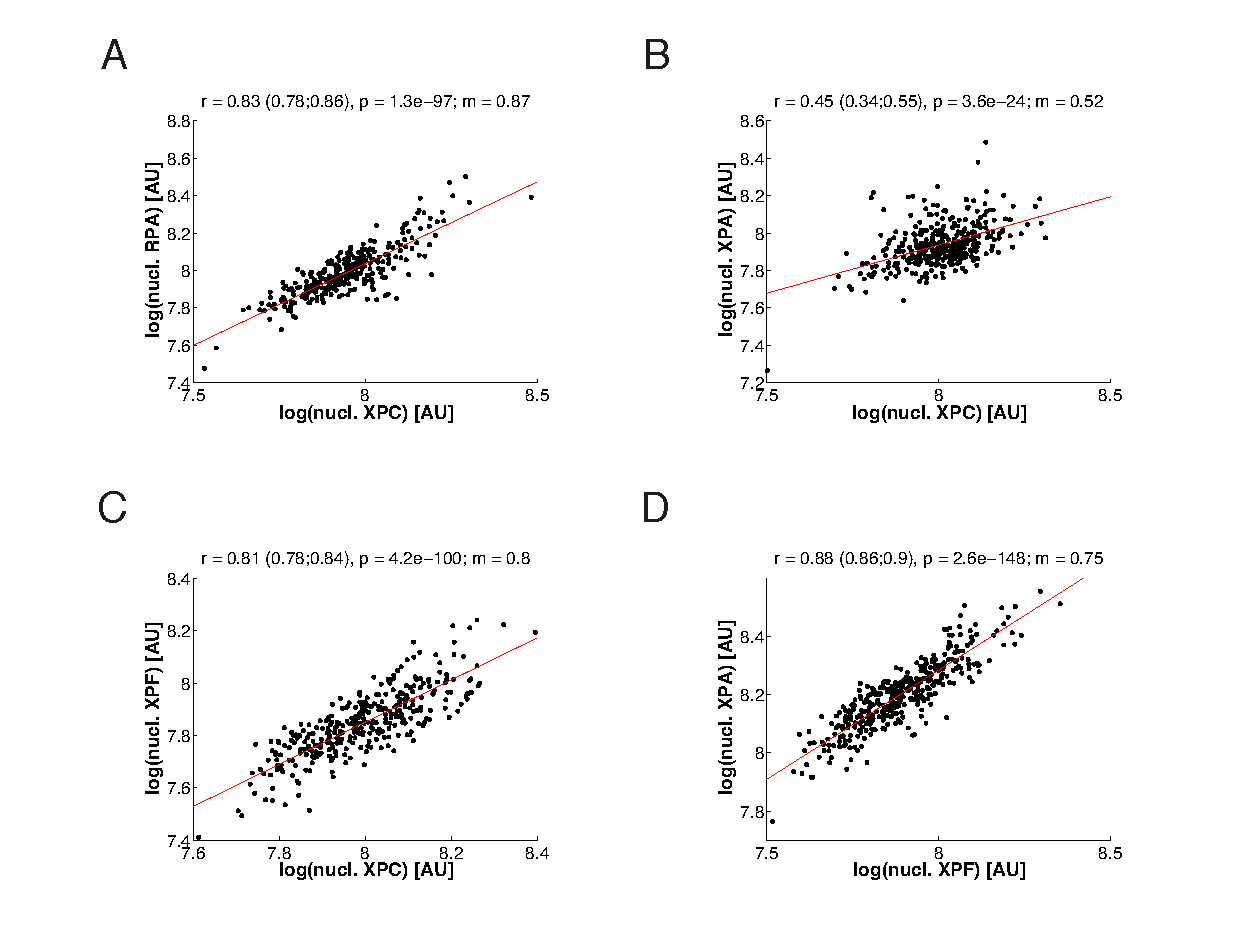
\includegraphics[width=1\textwidth]{Abbildungen/figure_A_2.pdf}
		\caption{\textbf{Nuclear expression of NER factors is correlated.} Pairwise correlations of indirectly antibody-labelled RPA against XPC (n=383, A), XPA against XPC (n=464, B), XPF against XPC (n=425, C) and XPA against XPF (n=454 , D) in locally damaged cells. Expression values represent fluorescence intensities originating from the nucleus including the damaged region. Red lines represent linear regression with correlation coefficient r, p-value and slope m. 95\% confidence bounds of all correlation coefficients r were estimated by non-parametric bootstrap and are given in brackets. }
		\label{fig:nuklearCrosscorrelation}
	\end{center}
\end{figure}


\begin{table}[H]
	
\begin{center}
	\begin{tabular}{llll}
		
		\multicolumn{4}{l}{} \\
		\hline
		\rule{0pt}{2ex}
		\hspace{-0.15cm}\textbf{Species}    &\textbf{Type} & \textbf{Protein} & \textbf{Manufacturer} \\
		\hline
		
		Mouse & mAb & RPA70 & Abcam       \\
		Mouse & mAb & XPC   & Abcam       \\
		Mouse & mAb & XPF & Abcam       \\
		Rabbit & pAb & XPB & Abcam       \\
		Rabbit & pAb & XPA & Abcam       \\
		\hline
	\end{tabular}
	\caption{\textbf{Primary antibodies.}  mAb = monoclonal antibody; pAb = polyclonal antibody}
	\label{tab:antibodies}
	\end{center}
\end{table}

\begin{table}[H]
	
\begin{center}
	\begin{tabular}{lllll}
		
		\multicolumn{5}{l}{} \\
		\hline
		\rule{0pt}{2ex}
		\hspace{-0.15cm}\textbf{Species}    &\textbf{Type} &\textbf{Fluorophore}& \textbf{Protein} & \textbf{Manufacturer} \\
		\hline
		
		Donkey & IgG (H+L) & Alexa488 & Mouse & Jackson Immunoresearch       \\
		Donkey & IgG (H+L) & Alexa647   & Mouse & Jackson Immunoresearch       \\
		Donkey & IgG (H+L) & Alexa647 & Rabbit& Jackson Immunoresearch       \\
		\hline
	\end{tabular}
	\caption{\textbf{Secondary antibodies.}  IgG (H+L) = Immunoglobulin G (Heavy + Light chains)}
	\label{tab:SecondaryAntibodies}
	\end{center}
\end{table}

\begin{table}[H]
\begin{center}
	\begin{tabular}{lllll}
		
		\multicolumn{5}{l}{} \\
		\hline
		\rule{0pt}{2ex}
		\hspace{-0.15cm}\textbf{Species}    &\textbf{Type} &\textbf{Fluorophore}& \textbf{Protein} & \textbf{Manufacturer} \\
		\hline
		Mouse & mAb & Alexa488 & XPC & Abcam       \\
		\hline
	\end{tabular}
	\caption{\textbf{Directly labelled antibody.}  mAb = monoclonal antibody}
	\label{tab:DirectlyLabeledAntibody}
	\end{center}
\end{table}


%\clearpage{\cleardoublepage}
%\clearpage{\pagestyle{plain2}} %\thispagestyle{empty}
%\clearpage{\pagestyle{empty}\cleardoublepage}


%\chapter*{Acknowledgements}
\addcontentsline{toc}{chapter}{Acknowledgements}
\thispagestyle{plain2}


An erster Stelle m\"ochte ich mich zutiefst bei meinem Betreuer Thomas H\"ofer f\"ur seine fortw\"ahrende Unterst\"utzung im Rahmen meiner Doktorarbeit  bedanken. Es lie\ss{}e sich nicht \"ubersch\"atzen, welch positiv inspirierenden Einfluss er auf diese Arbeit aber vor allem auch auf meine pers\"onliche wissenschaftliche Entwicklung genommen hat. \\

Ein gro\ss{}er Dank gilt Ursula Kummer und Frank Westermann f\"ur ihre kritische und zugleich motivierende Begleitung der Doktorarbeit als TAC-Mitglieder. Ursula Kummer gilt ein zus\"atzlicher Dank f\"ur ihre Rolle als Gutachterin der Arbeit und Vorsitzende des Pr\"ufungskomitees.\\

Ich bedanke mich sehr herzlich bei Prof. Ursula Klingm\"uller und Prof. Karsten Rippe f\"ur ihre Bereitschaft zur Teilnahme am Pr\"ufungskomitees.\\

Mein gr\"o\ss{}ter Dank gilt meiner Familie f\"{u}r ihren bedingungslosen R\"{u}ckhalt, ihr Vertrauen und ihr Liebe.\\

Ein herzliches Dankesch\"{o}n gilt Melanie, die nicht nur f\"{u}r meine gesunde Ern\"{a}rung, mein sportliches Wohlbefinden und meine regelm\"{a}\ss{}ige Teilnahme am Gruppenmeeting gesorgt hat, sondern auch eine gro\ss{}artige Freundin geworden ist. \\      

Ein weiterer gro\ss{}er Dank gilt Erika für ihre Freundschaft und für die vielen gemeinsamen Wanderungen um die Welt (und Heidelberg), die hoffentlich auch in Zukunft ihre Fortsetzung finden werden.\\

In ganz besonderem Ma\ss{}e m\"{o}chte ich mich bei Paul Verbruggen bedanken f\"ur seine Begeisterungsf\"{a}higkeit, seine Hartn\"{a}ckigkeit und seinen Humor, den er trotz des Amsterdamer Wetters nie verloren hat. Nicht oft hat man das Gl\"{u}ck mit einem Freund zusammenarbeiten zu d\"{u}rfen.\\

Einen gro\ss{}en Dank an Martin, der es trotz seiner Unerreichbarkeit irgendwie geschafft hat, immer f\"{u}r mich da zu sein.\\

Ich danke der gesamten Arbeitsgruppe H\"{o}fer f\"{u}r eine ausgesprochen angenehme Arbeitsatmosph\"{a}re.  
%\setcounter{chapter}{1}


\end{document}
